\documentclass[a4paper, twoside]{report}

%% Language and font encodings
\usepackage[english]{babel}
\usepackage[superscript,biblabel]{cite} %% Small superscript references
\usepackage[utf8x]{inputenc}
\usepackage[T1]{fontenc}

%% Sets page size and margins
\usepackage[a4paper,top=3cm,bottom=2cm,left=3cm,right=3cm,marginparwidth=1.75cm]{geometry}

%% Useful packages
\usepackage{amsmath}
\usepackage{amssymb}
\usepackage{graphicx}
\usepackage[colorinlistoftodos]{todonotes}
\usepackage[colorlinks=true, allcolors=blue]{hyperref}

%% Technical drawing package
\usepackage{tikz}
\usetikzlibrary{arrows,chains,matrix,positioning,scopes,decorations.pathmorphing,math}

%% Math commands for formatting
\newcommand{\matr}[1]{\mathbf{#1}}
\DeclareMathOperator{\diag}{diag}

\title{Directing Wave Propagation by Topological Perturbation in Metamaterials}
\author{Bernard Ting}

\begin{document}
\begin{titlepage}

\newcommand{\HRule}{\rule{\linewidth}{0.5mm}} % Defines a new command for the horizontal lines, change thickness here

%----------------------------------------------------------------------------------------
%	LOGO SECTION
%----------------------------------------------------------------------------------------


\includegraphics[width=8cm]{title/logo.png}\\[1cm] % Include a department/university logo - this will require the graphicx package
 
%----------------------------------------------------------------------------------------

\center % Center everything on the page

%----------------------------------------------------------------------------------------
%	HEADING SECTIONS
%----------------------------------------------------------------------------------------

\textsc{\LARGE BEng Individual Project}\\[1.5cm] % Name of your university/college
\textsc{\Large Imperial College London}\\[0.5cm] % Major heading such as course name
\textsc{\large Department of Computing}\\[0.5cm] % Minor heading such as course title

%----------------------------------------------------------------------------------------
%	TITLE SECTION
%----------------------------------------------------------------------------------------
\makeatletter
\HRule \\[0.4cm]
{ \huge \bfseries \@title}\\[0.4cm] % Title of your document
\HRule \\[1.5cm]
 
%----------------------------------------------------------------------------------------
%	AUTHOR SECTION
%----------------------------------------------------------------------------------------

\begin{minipage}{0.4\textwidth}
\begin{flushleft} \large
\emph{Author:}\\
\@author % Your name
\end{flushleft}
\end{minipage}
~
\begin{minipage}{0.4\textwidth}
\begin{flushright} \large
\emph{Supervisor:} \\
Prof. Richard Craster \\[1.2em] % Supervisor's Name
\emph{Second Marker:} \\
Dr. Christopher Ford
\end{flushright}
\end{minipage}\\[2cm]
\makeatother

% If you don't want a supervisor, uncomment the two lines below and remove the section above
%\Large \emph{Author:}\\
%John \textsc{Smith}\\[3cm] % Your name

%----------------------------------------------------------------------------------------
%	DATE SECTION
%----------------------------------------------------------------------------------------

{\large \today}\\[2cm] % Date, change the \today to a set date if you want to be precise

\vfill % Fill the rest of the page with whitespace

\end{titlepage}


\begin{abstract}
We first introduce the theory of dispersion curves and plot them for simple
models. We then break the symmetry by introducing masses of different weights
and observe how this affects the dispersion curves. We then investigate these
structures in the case of media composed of one symmetry breaking ribbon above
another. We use this to find special frequencies or modes which are present in
the band gap. Scattering simulations are run with these frequencies induced to
the lattice to confirm our analysis.
\end{abstract}

\renewcommand{\abstractname}{Acknowledgements}
\begin{abstract}
I would like to extend my greatest thanks to my supervisor, Prof. Richard
Craster, for his advice and guidance on all matters relating to the project. I
would also like to thank Dr. Christopher Ford for being my second marker and
providing timely feedback regarding my project.
\end{abstract}

\tableofcontents
%% \listoffigures
%% \listoftables

\chapter{Introduction}
The study of metamaterials has the potential to solve many modern engineering problems.
\section{Objectives}
\section{Challenges}
\section{Contributions}

\chapter{Background}
Waves exhibit many characteristics when travelling through different media.
Much research has been carried out to investigate and harness these properties
to develop technologies and devices which manipulate electromagnetic (photonic)
and also acoustic (phononic) waves.

\section{History}
Since the earliest days of human history, we have sought to better understand
the natural world around us and so create technologies to improve our lives. At
first by utilising what nature already has to offer, but later on developing
materials and devices which have desirable properties not found in nature.

This progression describes roughly how the study of metamaterials came about.
It began in 1887 with the study of how certain crystals exhibit interesting
iridescence.\cite{pcearliest} After two independently developed landmark papers
were published in 1987 on structures with band gaps for electromagnetic
waves,\cite{pceli,pcjohn} the term photonic crystal --- a periodic optical
nanostructure which manipulates the passage of electromagnetic radiation ---
was coined.\cite{pcfocus} Since then, photonic crystals have been mass produced
and used for many purposes, e.g. optical fibres for transmission of digital
information \cite{pcopfib} and precision surgery.\cite{pcsurgery,pcneuro}

Then came the study of metamaterials --- materials engineered to possess some
property not found in naturally occurring materials.\cite{briefintro} Usually
these materials are composed of smaller units which are arranged in a repeating
pattern. They derive their properties not from the intrinsic properties of the
base materials, but from the periodic structure introduced.

One of the first major breakthroughs which the study of metamaterials led to
was the development of materials with a negative refractive index. Though the
possibility of creating such a material was theoretically predicted in
1967,\cite{negrefrac} it was only experimentally verified in
2001.\cite{negrefracex}

Nowadays, there is much research being done in the area of topological
metamaterials or topological photonic
crystals.\cite{topoedge,toposplit,topomet} This is where new properties of
metamaterials are produced by perturbing their structures utilising topological
and group theoretic concepts, usually by breaking symmetries which are present
in the original material. The reason there is considerable interest in applying
these abstract fields to the study of metamaterials is due to their ability to
transcend specific physical systems and be applied widely. An example is being
able to create metamaterials which split energy in multiple
directions.\cite{toposplit} Since then, much research has been done in
emulating these topological effects in simpler systems and then transferring
the results into proper experimentation in the desired
contexts.\cite{elasticvhe,singlevalley,exobs,exobs2} This forms an exciting
modern area of wave physics and we mention below some of the novel applications
which can be realised with these systems.

\section{Practical applications}
\label{applications}
Metamaterials have the potential to solve many modern engineering problems.

\begin{itemize}
\item Developing a cloak of invisibility.\cite{emcloak}
      \begin{itemize}
      \item Obvious use cases in military.
      \item Protect things from electromagnetic radiation.
      \end{itemize}
\item Constructing antennae to focus energy into narrow beams.
      \cite{diremi,antennasol}
      \begin{itemize}
      \item Gather wave energy from deep in the oceans and concentrate them to
            be harvested.
      \item Channel sound energy, e.g. from train tracks, to be dissipated
            elsewhere which decreases noise pollution.
      \end{itemize}
\item Producing devices which operate on the terahertz ($1THz=10^{12}Hz$)
      range.\cite{THz}
      \begin{itemize}
      \item Can be used in medical imaging due to terahertz radiation being
            able to penetrate thin materials but not thicker objects. Also, it
            is non-ionising radiation and so does not damage living cells
            unlike X-rays.
      \item For surveillance, especially security screening as many materials
            of interest have unique spectral fingerprints in the THz
            range.\cite{Thzsec}
      \end{itemize}
\item Developing near perfect electromagnetic absorbers.\cite{absorbing}
\item Developing energy splitters.\cite{toposplit}
\item Developing perfect lenses.\cite{negrefraclens}
\end{itemize}

\section{Models studied}
There are many different models which we can use to study the effects of
metamaterials on the waves which propagate through them. 

\begin{figure}[!h]
\centering
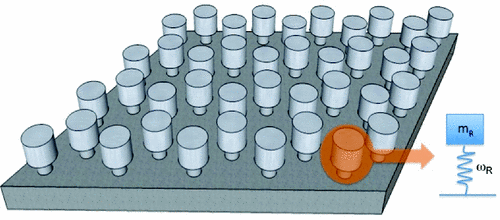
\includegraphics[width=0.8\textwidth]{imgs/flexplate.png}
\caption{\label{fig:flexplate} Schematic view of a thin plate flexural wave
         model which consists of an array of resonators attached to a thin
         elastic plate. Each resonator is a point mass attached to the plate by
         a spring. Image adapted from source.\cite{graphene}}
\end{figure}

In the literature, thin plate flexural wave theories,\cite{graff,toelastic} as
seen in Figure~\ref{fig:flexplate}, have proven to be highly effective physical
models and reliable predictors of physical wave phenomena as shown by the
numerous studies done on flexural (or bending) waves in a beam or a
plate.\cite{flexbeam,graphene,mehulgeom} This is very advantageous as most
acoustic (or sound) radiation travels as flexural waves through structures and
deforms the medium transversely as they propagate.\cite{sound} Therefore, these
models are very useful in studying acoustic metamaterials or phononic
crystals.\cite{phonon} As a specific example, an elastic analogue of graphene,
a honeycomb arrangement of mass-spring resonators attached to a thin elastic
plate, was shown which could be used as waveguides.\cite{graphene}

Having said that, the equations which govern the propagation of flexural waves
are much more complicated than those for a simple mass-spring system and
requires more background knowledge in its physics to properly understand and
implement. As an example, the biharmonic equation which governs the propagation
of flexural waves in a lattice of mass-spring resonators is a fourth-order
partial differential equation.

Along the same lines, the modelling of electromagnetic metamaterials present
the challenges of getting to grips with the theory of electromagnetic
radiation, e.g. Maxwell's equations\cite{maxwell} and Bragg
scattering\cite{bragg}.

\begin{figure}
\centering
  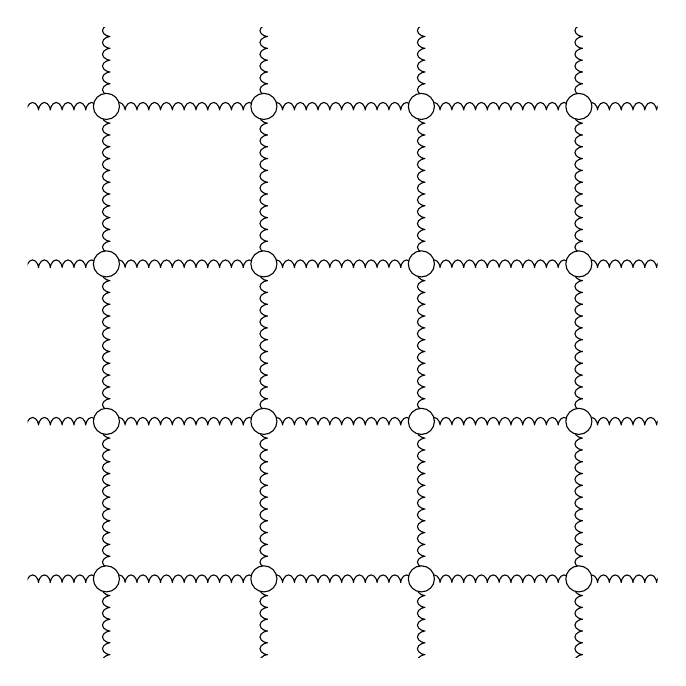
\begin{tikzpicture}
    \clip (-1,-1) rectangle (7,7);
    \foreach \X in {-2,0,...,6}
    {\foreach \Y in {-2,0,...,6}
     {\draw[decorate,decoration={coil,aspect=0.5,amplitude=0.5mm, segment
    length=1.5mm}] (\X,\Y) -- ++(0,2) -- ++(2,0);
    \node[circle,draw,inner color=white] at (\X,\Y) {};}}
  \end{tikzpicture}
  \caption{\label{fig:ourmodel} Schematic view of our simple mass-spring model.}
\end{figure}

Given the timeline of this project, the limited Physics background I have, as
well as to make the results accessible to a wider audience, we have decided to
go for a simplistic masses-connected-by-springs model, as seen in
Figure~\ref{fig:ourmodel}, as the core object of study in our project. The
lattice will be formed of repeating cells (e.g. Figure~\ref{fig:sqscheme}) and
it is the periodicity in the lattice which will give rise to its special
properties. Not only does this reduce the complexity as we only need to deal
with ordinary differential equations and not partial differential equations, it
also reduces the complexity in the scattering simulations as we now have to
solve a discrete system instead of a continuous one. With this \textit{toy}
system which form the basic building blocks of solid state physics, we will be
able to more quickly lay the foundations required to carry out more interesting
experiments, from which results can be transferred to other models.

The two lattices which we will be focusing most of this work on is the
hexagonal and kagome lattice. This is because they have a lot of physical
analogues which are particularly useful.\cite{singlevalley,wuandhu,kphysical}
As a concrete example, the kagome lattice shown in
Figure~\ref{fig:kagomescheme} has a physical analogue as a dense packed system
such as the one shown in Figure~\ref{fig:kagomephysical}. The dense packed
system consists of particles and voids filled with fluid connected by thin
gaps. The key to controlling the behaviour of the crystal is being able to
precisely engineer the thin gaps, as the gaps and voids together form a
connected network of resonators. Thus, it can be seen that our model is
asymptotically equivalent to this physical system.\cite{kphysical}

\begin{figure}[!h]
\centering
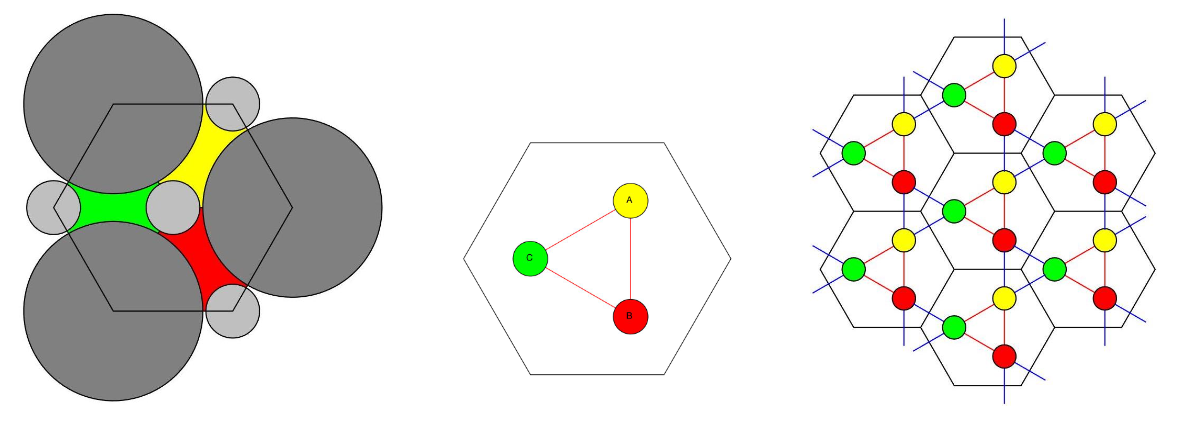
\includegraphics[width=0.8\textwidth]{imgs/kagomephysical.PNG}
\caption{\label{fig:kagomephysical} The closely packed system (left) shows
rigid cylindrical inclusions of two different radii, the elementary hexagonal
cell and the three voids (yellow, green, red) connected by thin gaps. The
asymptotically equivalent Kagome lattice as a discrete network model (right).
Image and caption adapted from source.\cite{kphysical}.}
\end{figure}

The following will be brief explanations of concepts which will form the
foundation on which we will analyse and investigate the properties of our
lattices.

\section{Dispersion relation}
\label{disperbg}
A dispersion relation relates the wavenumber of a wave to its frequency. We
will see that this relation is of utmost importance when discussing periodic
lattices as only waves of certain frequencies are transmitted by the lattice
and the dispersion relation directly shows us which frequencies these are. As
we will be solving for the dispersion relation of infinite and semi-infinite
lattices in Chapter \ref{disperrel} and \ref{perturbed}, we will be making use
of the concepts below to simplify the problem (because we do not want to solve
an infinite problem!).

\section{Bloch waves}
\label{blochbg}
Bloch's theorem for waves in a periodic potential\cite{bloch} states that any
wave travelling through a periodic potential can be expressed as the product of
a periodic function and a plane wave,\cite{kittel} i.e.

\begin{align}
  \psi_{\vec{\kappa}}(\vec{r})=f_{\vec{\kappa}}(\vec{r})e^{i\vec{\kappa}\cdot\vec{r}}
\label{eq:blochwave}
\end{align}

where $f_{\vec{\kappa}}(\vec{r})$ has the period of the lattice with
$f_{\vec{\kappa}}(\vec{r})=f_{\vec{\kappa}}(\vec{r}+\vec{R})$, with $\vec{R}$ being a
translation vector of the lattice.

The proof of this theorem can be found here.\cite{kittel} But we will just
state how we can use this result to simplify the equations we will obtain in
our systems. This is useful for us as we are modelling elastic waves travelling
through a periodically-repeating mass-spring system and so Bloch's theorem
applies. Thus we can write the displacement of one mass as the displacement of
another corresponding mass in the lattice with a complex exponential factor. By
doing this, we can characterise the behaviour of all the displacements by just
focusing on finding the displacements of masses in the \textit{primitive cell},
which is just the unit cell which forms the repeating base of our lattice. We
will see later how this helps to reduce our infinite system of equations down
to a finite number, such as in \eqref{eq:HLN2L} and \eqref{eq:blochsq}.

\section{Reciprocal lattice}
\label{reclatbg}
A reciprocal lattice represents the Fourier transform of another lattice. In
our case, our model lattice is a periodic spatial function in real space, and
so its reciprocal lattice exists as a function of frequency in reciprocal
space.  We will continue with a more formal explanation based on the materials
in the Appendix of this book,\cite{moldinglight} restricting our discussion to
only 2-dimensional lattices which is sufficient for our purposes.

More formally, suppose we have a function $f(\vec{r})$ which is periodic on a
lattice, i.e. $f(\vec{r})=f(\vec{r}+\vec{R})$ for all vectors $\vec{R}$
that translate the lattice onto itself (connect a lattice point to the next).
Then we call $\vec{R}$ the \textit{lattice vectors}. As we shall see later,
elastic waves travelling through our mass-spring lattices are examples of such
a periodic function. Naturally then, we would take the Fourier transform when analysing a periodic function, i.e.

\begin{align}
  f(\vec{r})=\int c\vec{q}g(\vec{q})e^{i\vec{q}\cdot\vec{r}}
\end{align}

Applying periodicity, we see that

\begin{align}
  &f(\vec{r}+\vec{R})=f(\vec{r}) \\
  &\Rightarrow\int c\vec{q}g(\vec{q})e^{i\vec{q}\cdot\vec{r}}e^{i\vec{q}\cdot\vec{R}}=\int c\vec{q}g(\vec{q})e^{i\vec{q}\cdot\vec{r}} \\
  &\Rightarrow g(\vec{q})=g(\vec{q})e^{i\vec{q}\cdot\vec{R}}
\end{align}

Therefore, this tells us that the transform $g(\vec{q})$ has to be zero
everywhere, except where $e^{i\vec{q}\cdot\vec{R}}=1$, or equivalently
$\vec{q}\cdot\vec{R}=2\pi N$ for any $N\in \mathbb{Z}$. These vectors $\vec{q}$ that
satisfy this condition are called the \textit{reciprocal lattice vectors} and
are usually designated by $\vec{G}$. Note also that these reciprocal lattice
vectors form a lattice of their own, which we can easily verify as

\begin{align}
(\vec{G}_1+\vec{G}_2)\cdot\vec{R}=\vec{G}_1\cdot\vec{R}+\vec{G}_2\cdot\vec{R}=2\pi (N_1+N_2)
\end{align}
 
and we call this reciprocal lattice the \textit{reciprocal space}.

So given a set of lattice vectors $\vec{R}$, to find the reciprocal lattice
vectors $\vec{G}$, we need to find all $\vec{G}$ such that
$\vec{G}\cdot\vec{R}$ is some integer multiple of $2\pi$ for every $\vec{R}$.
Since we know that $\{\vec{G}\}$ forms a lattice, we know that every reciprocal
lattice vector $\vec{G}$ can be written as $\vec{G}=l\vec{b_1}+m\vec{b_2}$ for
some set of primitive lattice vectors $\vec{b}_i$, similar to how any lattice
vector $\vec{R}$ can be written as $\vec{R}=p\vec{a_1}+q\vec{a_2}$ for some set
of primitive lattice vectors $\vec{a}_i$ which are the smallest vectors
pointing from one lattice point to another and need not be of unit length.
Therefore 

\begin{align}
  &\vec{G}\cdot\vec{R}=2\pi N \\
  &\Rightarrow (p\vec{a}_1+q\vec{a}_2)\cdot(l\vec{b}_1+m\vec{b_2})=2\pi N
\end{align}

From this, it is easy to see that constructing $\vec{b}_i$ such that
$\vec{a}_i\cdot\vec{b}_j=2\pi\delta_{ij}$ satisfies the above condition.
Therefore we see from this that if $\vec{a}_i$ is of length $a$, then
$\vec{b}_i$ will be of length $\frac{2\pi}{a}$, which is where the term
\textit{reciprocal} lattice is derived from.

\section{Brillouin zone}
\label{brizones}

The concept of Brillouin zones was first defined by Leon Brillouin in his book
on wave propagation in periodic structures.\cite{brillouin} As we are able to
tessellate our physical lattice with a periodically repeating unit cell, so
there exists a unit reciprocal cell which can cover the reciprocal space
without overlap. We will now motivate the selection of the first Brillouin zone
as a \textit{good} unit reciprocal cell based on the the discussions in
here.\cite{moldinglight}

To see how we might make a good choice for a unit cell for the reciprocal
space, notice that for the Bloch states (as defined in Chapter \ref{blochbg}),
different values of $\vec{\kappa}$ do not necessarily lead to different modes.
To be more precise, the modes with wave vector $\vec{\kappa}$ and
$\vec{\kappa}+2\pi N$ are identical, which means that $\vec{\kappa}$
essentially functions as the phase relationship between the displacement of
masses in our lattice. Now notice also that from \eqref{eq:blochwave} and the
fact that our lattice is periodic, we have that if $\vec{G}$ is a reciprocal
lattice vector (as defined in Chapter \ref{reclatbg}), then
$\vec{\kappa}+\vec{G}$ causes the phase difference between masses to be
incremented by $\vec{G}\cdot\vec{R}$ which we know is $2\pi N$ and so is no
difference at all!

This shows us that there is a lot of redundancy in $\vec{\kappa}$ and we do not
actually need to explore the whole of $\kappa$-space but it is enough for us to
restrict ourselves to a finite \textit{zone} in the reciprocal space from which
we \textit{cannot} get from one part of the lattice to area to another by
adding $\vec{G}$. This is visually demonstrated in Figure~\ref{fig:kappaspace}.

\begin{figure}[!h]
\centering
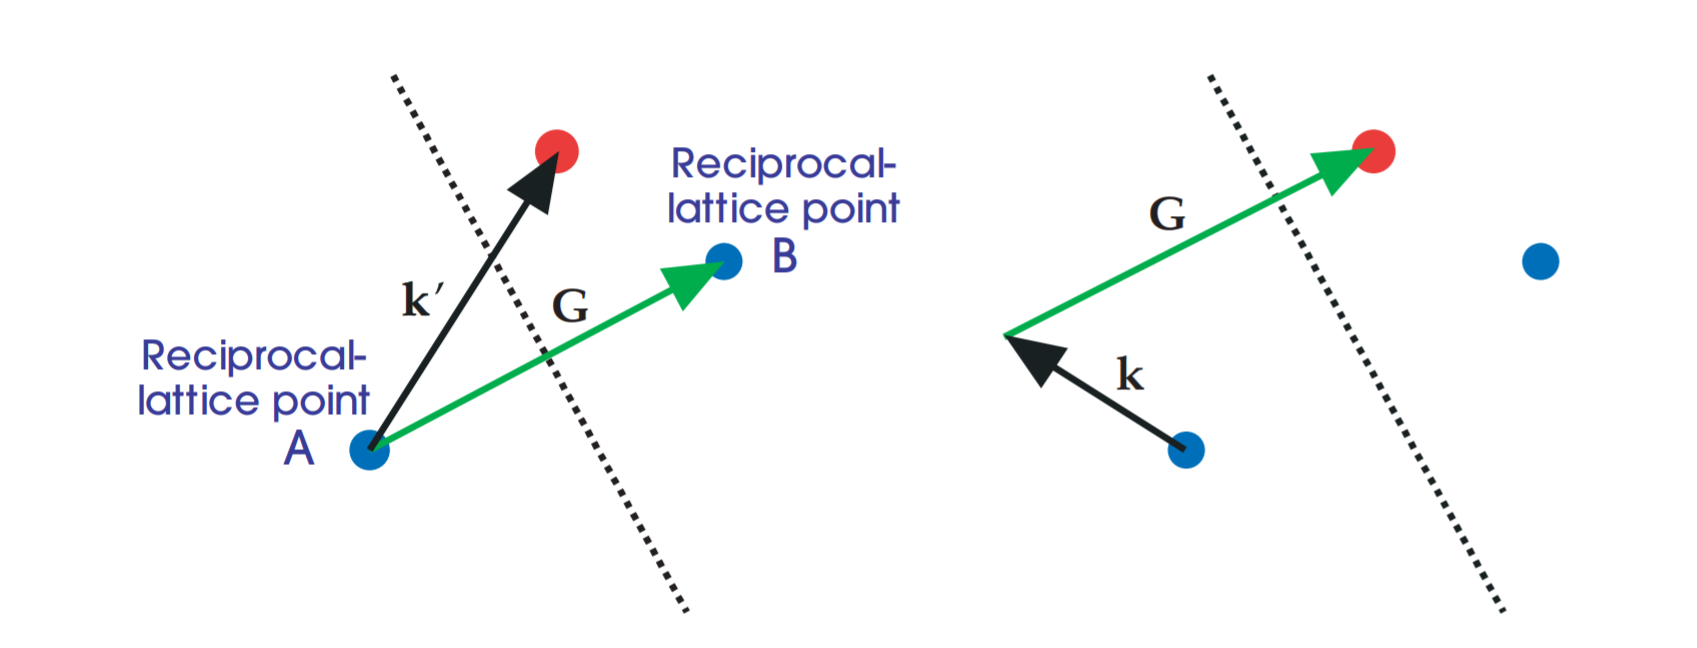
\includegraphics[width=0.8\textwidth]{imgs/kappaspace.PNG}
\caption{\label{fig:kappaspace} Characterisation of the Brillouin zone. The
  dotted line refers to the perpendicular bisector of the line joining two
  reciprocal lattice points (blue). Notice that if we choose the left point A
  as the origin, any lattice vector (such as $\vec{\kappa'}$) that reaches to
  an arbitrary point on the other side (red) can be expressed as the sum of a
  vector on the same side (such as $\vec{kappa}$) plus a reciprocal lattice
  vector $\vec{G}$. Image and caption adapted from source.\cite{moldinglight}.}
\end{figure}

There are many such zones, but we choose to focus on the region which is
closest to the origin, where $\vec{\kappa}=0$. And that zone is what we call
the first Brillouin zone. 

That is why the other way to define a Brillouin zone is that it is a particular
choice of this reciprocal cell and is constructed as the set of points enclosed
by the Bragg planes. The Bragg planes exist in reciprocal space and are the
planes perpendicular to a straight line from the origin to each lattice point.
The first Brillouin zone is then defined as the set of points formed by the
Bragg planes closest to the origin. These concepts are described visually for a
2d square real lattice in Figure~\ref{fig:bzonesq}.

The idea of Brillouin zones is brilliant in that now we know we only need to
solve for the dispersion relation for $\vec{\kappa}$ in the first Brillouin
zone to know the dispersion relation across the entire lattice.

\chapter{Dispersion relation}
\label{disperrel}
A dispersion relation relates the wavenumber of a wave to its frequency. We
will see that this relation is of utmost importance when discussing periodic
lattices as only waves of certain frequencies are transmitted by the lattice.

\section{1d lattice}
\begin{figure}[!h]
\begin{center}
  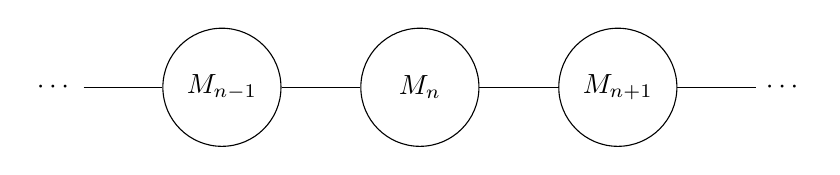
\begin{tikzpicture}
  {[start chain,every on chain/.style=join,every join/.style=-,
    state/.style={circle,draw,minimum size=1.5cm}]
     \node[on chain] (A) {$\cdots$};
     \node[on chain,state] (B) {$M_{n-1}$};
     \node[on chain,state] (C) {$M_n$};
     \node[on chain,state] (D) {$M_{n+1}$};
     \node[on chain] (E) {$\cdots$};
  }
  \end{tikzpicture}
  \caption{\label{fig:sqscheme1d} Schematic view of our 1d model.}
\end{center}
\end{figure}

Let us start our discussion with the most basic one-dimensional case. In this
case, we have masses of equal mass, $m$ spread out evenly across one dimension.
All neighbouring masses are connected by an elastic force which scales
proportionally with distance, i.e. $F = kx$ for some $k$.

% TODO: Add discussion about transverse waves into appendix?
\textit{Note}: As mentioned before, we will be thinking of this system as a
mass-spring system. Notice however that it does not matter whether we are
considering longitudinal or transverse waves, as the equations governing their
interactions are the same. In our discussions, we will be considering the waves
propagating through our models as transverse waves. This helps to simplify
visualisations as the displacements and movements of the masses are
perpendicular to the lattice on which they are bound.

With this one-dimensional case set up, we now want to find out what forms of
waves it allows to propagate. We do this by considering only nearest neighbour
interactions and examining the elementary unit of the lattice which can be
repeated by translation to form the full lattice.

So let us consider three masses side-by-side in our lattice, $M_{n-1}$, $M_n$
and $M_{n+1}$ which are $y_{n-1}$, $y_n$ and $y_{n+1}$ displacement away from
their equilibrium positions. By focusing on the centre mass and considering
only nearest neighbour interactions, by Hooke's Law, we have that the force on
$M_n$

\begin{align}
  F_{n}=\sum F=k\left(y_{n-1}+y_{n+1}-2y_{n}\right) \label{eq:HL}
\end{align}

At the same time, we have by Newton's 2nd Law that

\begin{align}
  F_{n}=m\frac{d^{2}}{dt^{2}}y_{n}
\end{align}

Taking $y_n$ to be the general wave solution

\begin{align}
  &y_{n}=\hat{y}_{n}e^{-i\Omega t} \\
  \Rightarrow &\frac{d^{2}}{dt^{2}}y_{n}=-\Omega^{2}y_{n} \\
  \Rightarrow &F_{n}=-m\Omega^{2}y_{n} \label{eq:N2L}
\end{align}

where $\Omega$ is the frequency of the wave and $\hat{y}_{n}$ is the complex
amplitude.

Therefore, we have by \eqref{eq:HL} and \eqref{eq:N2L} that

\begin{align}
  &-m\Omega^{2}y_{n}=k\left(y_{n-1}+y_{n+1}-2y_{n}\right) \\
  \Rightarrow &\left(-\frac{m}{k}\Omega^{2}+2\right)y_{n}-y_{n-1}-y_{n+1}=0
    \label{eq:HLN2L}
\end{align}

Since we can write this differential equation for any of our masses in our
infinite lattice, we would need to solve an infinite number of coupled second
order differential equations. However, the trick we use is that since we have
that $M_{n-1}$ and $M_{n+1}$ are equidistant from $M_{n}$ at equilibrium (i.e.
the lattice is periodic), we can make use of Bloch's theorem\cite{bloch} to
describe the phase shift in the wave solution as

\begin{align}
  y_{n-1}=e^{-i\kappa}y_n,\ \ y_{n+1}=e^{i\kappa}y_n
\end{align}

Hence, from \eqref{eq:HLN2L}, we see that

\begin{align}
  &\left(-\frac{m}{k}\Omega^{2}+2-e^{-i\kappa}-e^{i\kappa}\right)y_{n}=0 \\
  \Rightarrow &\cos\left(\kappa\right)=-\frac{m}{2k}\Omega^{2}+1
\end{align}

Therefore, we now have an equation linking the wave number $\kappa$ and the
frequency $\Omega$ of waves propagating across our 1d lattice. By initialising
$m$ and $k$ we can use this equation to plot the dispersion curve of our
system. By setting $m=k=1$, we get the dispersion curve in Figure
~\ref{fig:dc1}.

\begin{figure}[!h]
\centering
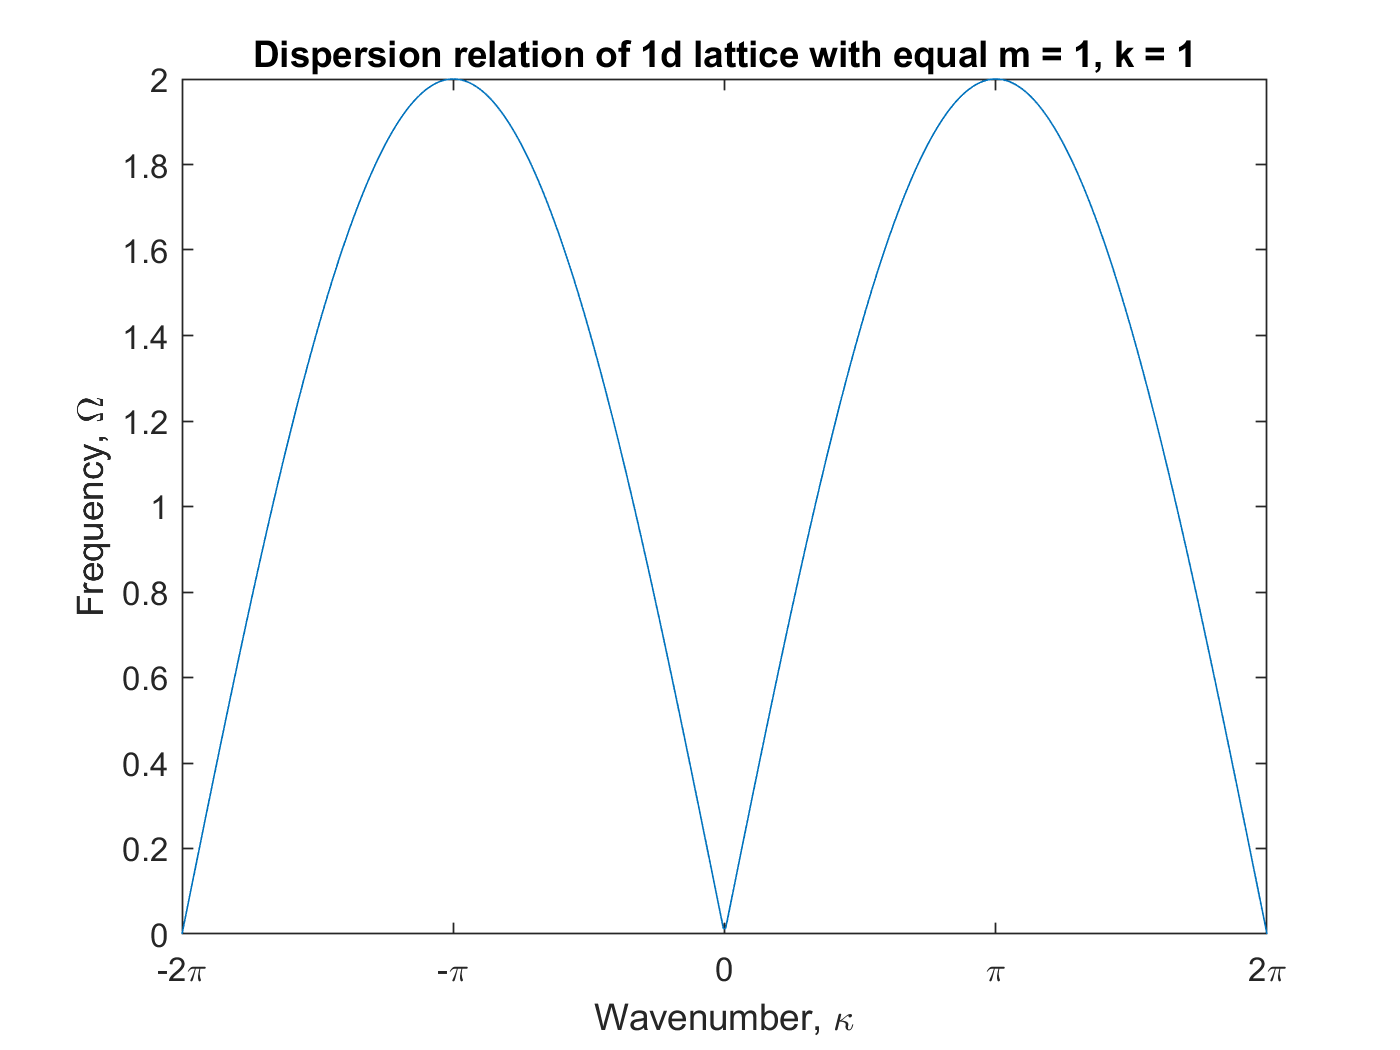
\includegraphics[width=0.8\textwidth]{imgs/1ddispersion.png}
\caption{\label{fig:dc1}Dispersion relation of a 1d monoatomic
         chain.}
\end{figure}

The first interesting thing to notice about this dispersion relation is that
the curve seems to be periodically repeating. More precisely, if we look at the
curve between $-\pi$ and $\pi$, we can see that translating this portion of the
graph left or right by $2\pi$ will give us the rest of the dispersion relation.
This range of wave numbers is known as the first Brillouin zone, which we will
discuss more in the context of 2d lattices in Chapter \ref{brizones}.

\section{2d square lattice}
\begin{figure}[!h]
\centering
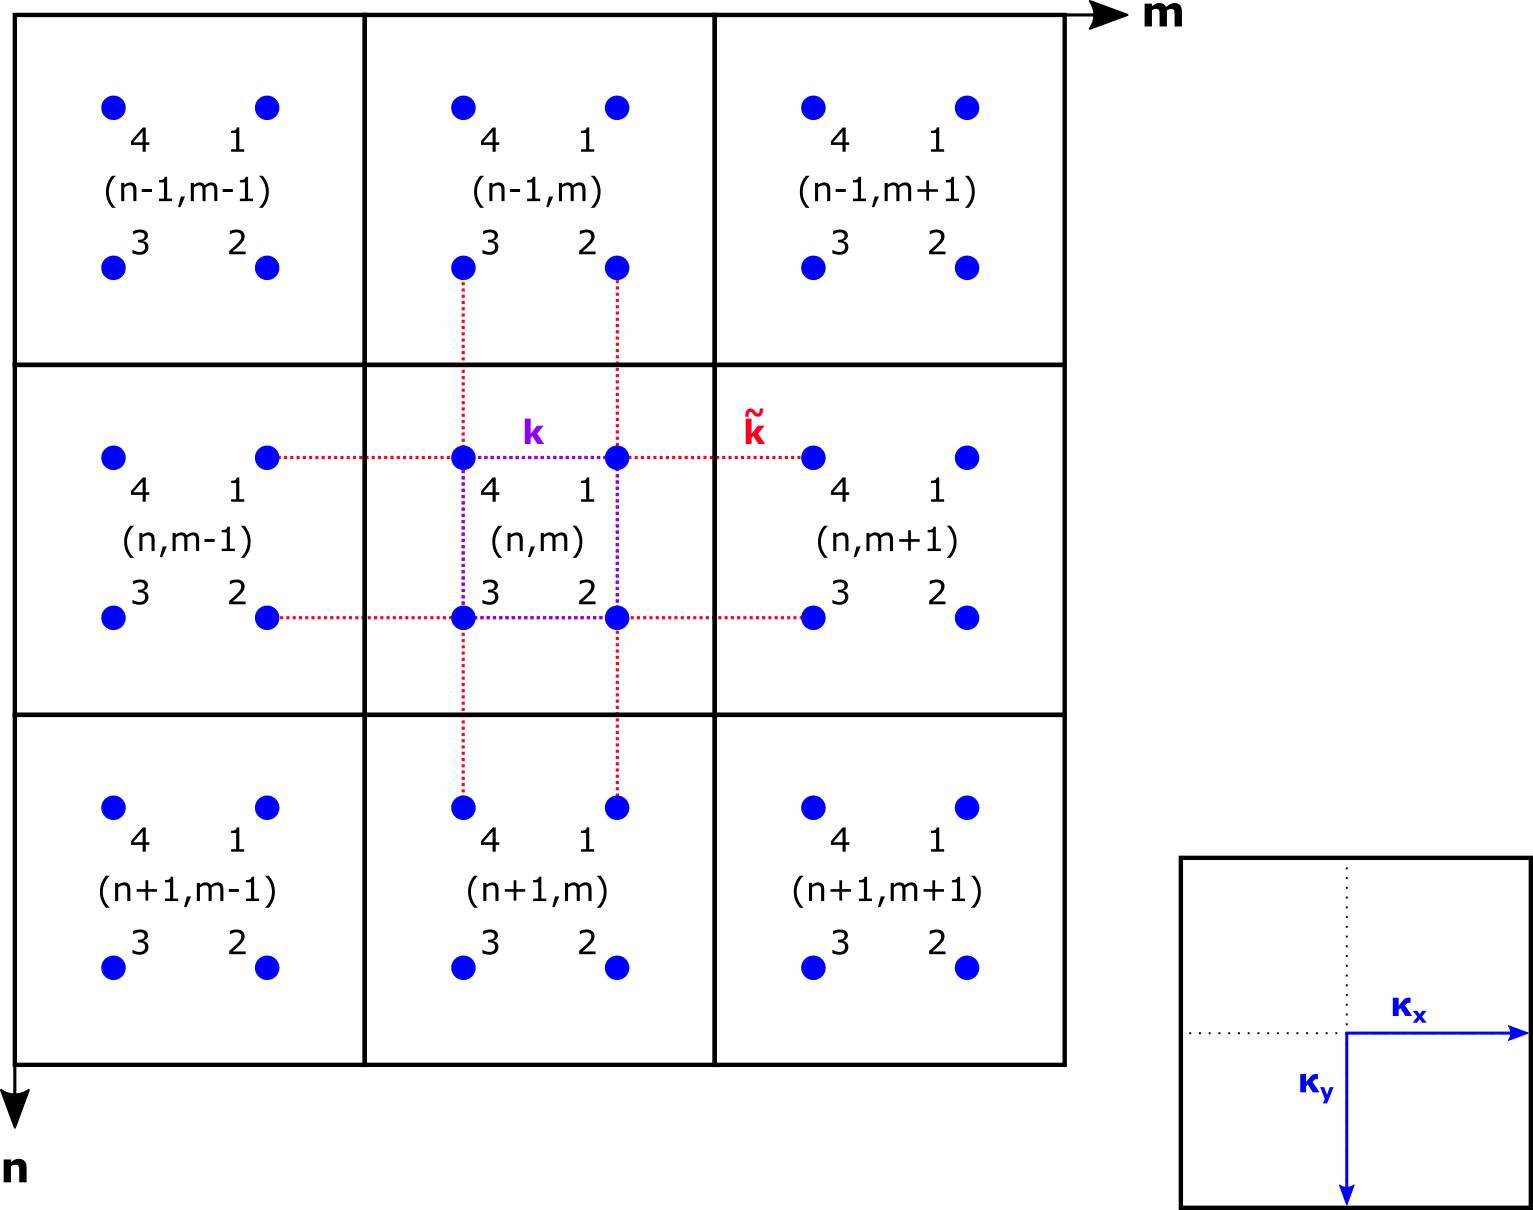
\includegraphics[width=0.8\textwidth]{imgs/sqmodel.png}
\caption{\label{fig:sqscheme} Schematic view of our 2d model. Each square
  tile in the grid corresponds to one elementary cell with four masses. $k$ and
  $\tilde{k}$ represent the intra- and inter-cell spring constants
  respectively. The cell in the far bottom right shows the directions of the
  Bloch phases. Note that only the elastic interactions involving the masses in
  cell $(n,m)$ are shown to avoid cluttering the figure, although they exist
  within and between each cell.}
\end{figure}

We now extend this analysis to an infinite two-dimensional square lattice, as
described in Figure~\ref{fig:sqscheme}. Each elementary square cell contains
four masses $M_i$ for $i\in\left[1, 4\right]$ which are arranged clockwise from
the top right. We take $n$ and $m$ to be the vertical and horizontal directions
respectively, with $n$ increasing downwards and $m$ increasing to the right, so
that relative to cell $(n, m)$ we have cell $(n-1,m)$ above and cell $(n,m+1)$
to the right. We have decided to go with this convention as it reflects matrix
indexing in Matlab, which will simplify our code. With this setup, we can now
label each mass and its displacement uniquely, e.g. $M_i$ in cell $(n, m)$ is
labelled $M_i^{n,m}$ and has displacement $y_i^{n,m}$.

\textit{Note:} Though we use this system to refer to specific masses in
specific cells, the mass of each mass is determined solely by its position in
its cell, i.e. $\forall n,m\in\mathbb{Z}$, the mass of $M_i^{n,m}=M_i$.

Each mass is elastically connected to its direct neighbours, e.g. $M_1^{n,m}$
is connected to $M_2^{n,m}$, $M_4^{n,m}$, $M_2^{n-1,m}$ and $M_4^{n,m+1}$. We
have the spring constant $k$ between masses in the same cell and $\tilde{k}$
between masses in adjacent cells.

Now again we consider only nearest neighbour interactions. Focusing on the
elementary cell $(n,m)$ and its adjacent cells, using Hooke's law and Newton's
2nd law on each of the masses in cell $(n,m)$, we can get a second order
differential equation which is coupled to the displacements of the other masses
it is connected to. For example, considering $M_1^{n,m}$, we get

\begin{align}
  F_1=M_1\frac{d^{2}}{dt^{2}}y_1^{n,m}
      =k\left(y_2^{n,m}+y_4^{n,m}-2y_1^{n,m}\right)+
       \tilde{k}\left(y_2^{n-1,m}+y_4^{n,m+1}-2y_1^{n,m}\right)
\label{eq:2dM1}
\end{align}

Since we can write this differential equation for any of our masses in our
infinite lattice, we would get an infinite number of coupled second order
differential equation. However, similar to the 1d case, using the periodicity
of the lattice and Bloch's theorem once more, we can relate the displacements
of each mass to the corresponding mass in a \textit{base cell} with the lattice
vectors $\kappa_y$ and $\kappa_x$, i.e.

\begin{align}
  y_i^{n+N,m+M}=e^{i\left(N\kappa_y+M\kappa_x\right)}y_i^{n,m}\ \ \ \ 
      \forall N,M\in\mathbb{Z}
\end{align}

With this, instead of an infinite number of equations, we have a set of four
coupled second order differential equations, one for each $y_i^{n,m}$ for
$i\in\left[1,4\right]$. We now drop the superscripts $\left(n,m\right)$ and
assume we have a wave solution of the form  

\begin{align}
  &y_{i}=\hat{y}_{i}e^{-i\Omega t} \\
  \Rightarrow &\frac{d^{2}}{dt^{2}}y_{i}=-\Omega^{2}y_{i} \\
  \Rightarrow &F_{i}=-M_i\Omega_i^{2}y_{i}
\label{eq:wavesol}
\end{align}

where $\Omega$ is the frequency of the wave and $\hat{y}_{n}$ is the complex
amplitude. We can now rewrite \eqref{eq:2dM1} as

\begin{align}
  M_1\Omega_1^{2}y_1
      &=k\left(2y_1-y_2-y_4\right)+
       \tilde{k}\left(2y_1-y_{2}e^{-i\kappa_y}-y_{4}e^{i\kappa_x}\right) \\
      &=\left(2k+2\tilde{k}\right)y_1+\left(-k-\tilde{k}e^{-i\kappa_y}\right)y_2+
       \left(-k-\tilde{k}e^{i\kappa_x}\right)y_4
\end{align}

By constructing this equation for each $y_i$, we can reformulate these four
difference equations as an eigenvalue problem

\begin{align}
  \left[\matr{A}\left(\kappa_{x},\kappa_{y}\right)-\matr{\Omega}\matr{M}\right]\vec{y}=\vec{0}
\label{eq:sqeig}
\end{align}

where $\matr{\Omega}=\diag\left(\left\{\Omega_i^2\right\}\right)$,
$\matr{M}=\diag\left(\left\{M_i\right\}\right)$,
$\vec{y}=\left[\left\{y_i\right\}\right]^T$ and

\begin{align}
  \matr{A}\left(\kappa_{x},\kappa_{y}\right)=\left[
\begin{array}{cccc}
2k+\tilde{k} & -k-\tilde{k}e^{-i\kappa_{y}} & 0 & -k-\tilde{k}e^{i\kappa_{x}}\\
-k-\tilde{k}e^{i\kappa_{y}} & 2k+\tilde{\tilde{k}} & -k-\tilde{k}e^{i\kappa_{x}} & 0\\
0 & -k-\tilde{k}e^{-i\kappa_{x}} & 2k+\tilde{\tilde{k}} & -k-\tilde{k}e^{i\kappa_{y}}\\
-k-\tilde{k}e^{-i\kappa_{x}} & 0 & -k-\tilde{k}e^{-i\kappa_{y}} & 2k+\tilde{\tilde{k}}
\end{array}\right]
\end{align}

Therefore, we can solve for the eigenvalues and eigenvectors of this equation.
The eigenvalues of this equation correspond to the frequency of waves,
$\Omega$, which are allowed through our lattice while the eigenvectors
correspond to the displacement of the masses, $y_i$. However, the next question
arises: How should we vary $\kappa$ so that we get a good enough picture of the
full dispersion relation of our 2d lattice?

To answer this question, we first have to discuss the theory of Brillouin zones.

\subsection{Brillouin zones}
\label{brizones}
%TODO: Molding the flow of light might be useful
The concept of Brillouin zones was first defined by Leon Brillouin in his book
on wave propagation in periodic structures.\cite{brillouin} The Brillouin zone
is a particular choice of the unit cell of the reciprocal lattice, where a
reciprocal lattice represents the Fourier transform of another lattice. In our
case, our model lattice is a periodic spatial function in real space, and so
its reciprocal lattice exists as a function of frequency in reciprocal space.

As we are able to tessellate our physical lattice with a periodically repeating
unit cell, so there exists a unit reciprocal cell which can cover the
reciprocal space without overlap. A Brillouin zone is a particular choice of
this reciprocal cell and is constructed as the set of points enclosed by the
Bragg planes. The Bragg planes exist in reciprocal space and are the planes
perpendicular to a straight line from the origin to each lattice point. These
concepts are described visually for a 2d square real lattice in
Figure~\ref{fig:bzonesq}.

\begin{figure}[!h]
\centering
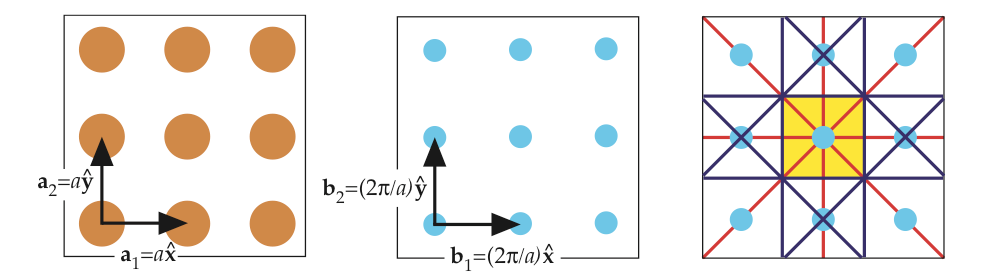
\includegraphics[width=0.8\textwidth]{imgs/bzonesq.png}
\caption{\label{fig:bzonesq} On the left is the lattice points in real space.
    In the middle is the corresponding reciprocal lattice. On the right is the
    construction of the first Brillouin zone: straight lines are drawn from the
    origin to the other lattice points (red), their perpendicular bisectors are
    the Bragg planes (blue), and the innermost region enclosed by the Bragg
    planes is the first Brilloin zone (yellow). Image and caption adapted from
    source.\cite{MITnp}}
\end{figure}
%TODO: Explain image equations?

Now that we have a uniquely defined unit cell in the reciprocal lattice, we
only have to consider solutions which occur in this region, as all distinct
Bloch waves occur within the first Brillouin zone. To simplify it even further,
there is a related concept called the irreducible Brillouin zone, which is the
first Brillouin zone reduced by the all of its symmetries. This can be seen for
the 2d square lattice in Figure~\ref{fig:ibzonesq}.
%TODO: Cite theorem of proof that ^ is true

\begin{figure}[!h]
\centering
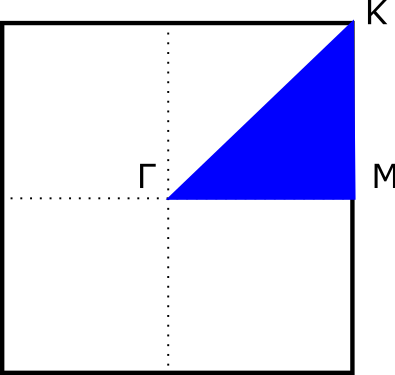
\includegraphics[width=0.3\textwidth]{imgs/sqibz.png}
\caption{\label{fig:ibzonesq} The irreducible Brillouin zone of the 2d square
    lattice in reciprocal space (blue).}
\end{figure}

With these concepts, we can fully solve the dispersion relation over our
infinite lattice space by just finding the solutions within the irreducible
Brillouin zone. Even more, given that standing waves are only present on the
boundary of the irreducible Brillouin zone, we only need to solve the
dispersion relation over the boundary.
%TODO: Is it because of standing waves??

Therefore for this case of an infinite 2d square lattice, we first solve the
eigen-problem we have in \eqref{eq:sqeig} over the boundary of the irreducible
Brillouin zone as shown in Figure~\ref{fig:ibzonesq}. We do this in Matlab by
varying the values of $\kappa_{x}$ and $\kappa_{y}$ which correspond to the
locus of points on the boundary of the irreducible Brillouin zone, and then
solve the eigen-problem for the eigenvalues and eigenvectors, which represent
$\matr{Omega}$ and $\vec{y}$ respectively. Then, we get the dispersion relation
by plotting out $\Omega_i$ against $(\kappa_x,\kappa_y$ or the position on the
Brillouin zone.

\textit{Note}: The significance of the eigenvectors or $y_i$ will be discussed
more in Chapter \ref{}.
%TODO: Do we need to use the eigenvectors?

We first need to find the values of $\kappa_{x}$ and $\kappa_{y}$ at $\Gamma$,
$X$ and $M$ as shown in Figure~\ref{fig:ibzonesq}.
%TODO: What should the limits of kappa_x and kappa_y be?

With this, and assuming that all masses $M_i=1$ for now (we will explore how
different perturbations in the lattice affect the dispersion relation in
Chapter \ref{perturbed}), we get the dispersion relation in
Figure~\ref{fig:sqdisper}. 
%TODO: Plot dispersion relation of 2d square lattice and explain?

\section{2d hexagonal lattice}
\label{2dhexdisper}
We will now consider how waves propagate across a 2d lattice made of hexagonal
elementary cells. 

\begin{figure}[!h]
\centering
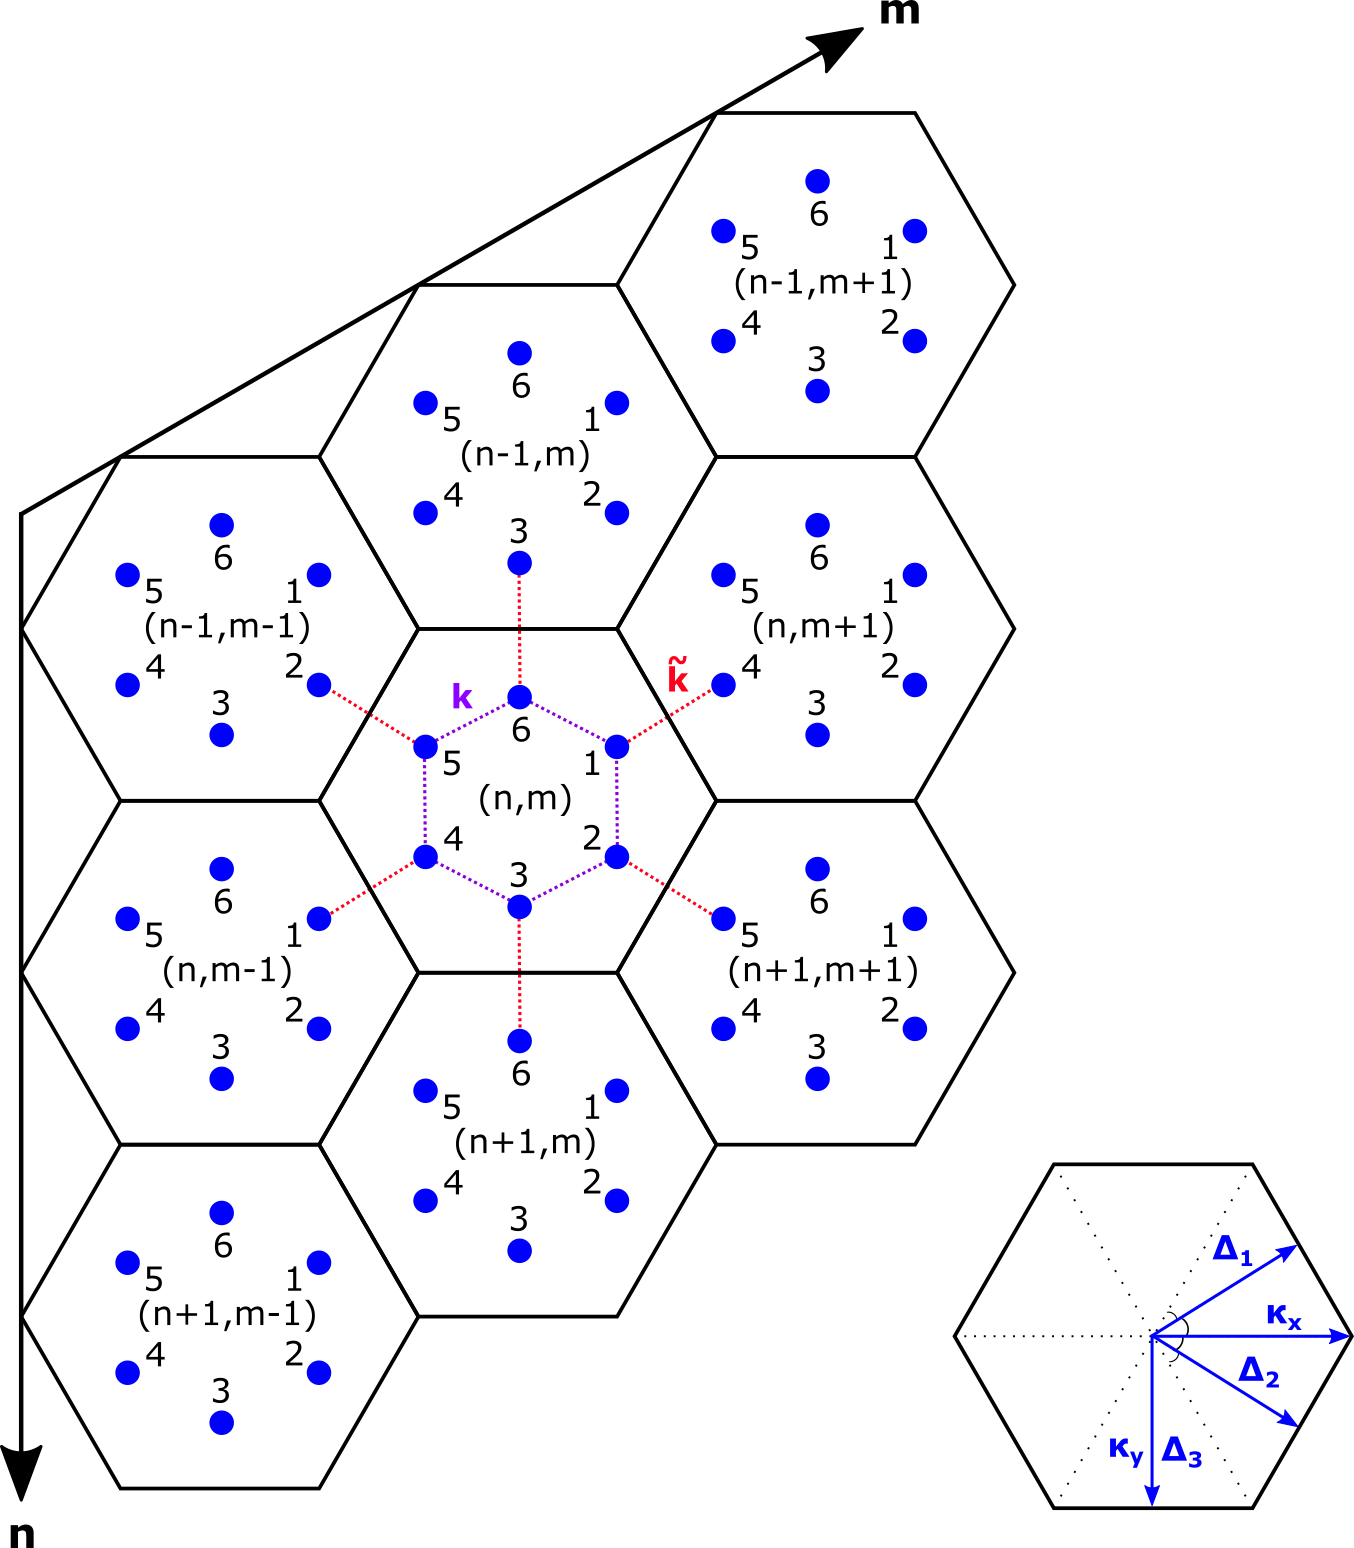
\includegraphics[width=0.8\textwidth]{imgs/hexmodel.png}
\caption{\label{fig:hexscheme} Schematic view of our 2d hexagonal model. Each
  hexagonal tile in the grid corresponds to one elementary cell with six
  masses. $k$ and $\tilde{k}$ represent the intra- and inter-cell spring
  constants respectively. The cell in the far bottom right shows the directions
  of the Bloch phases. Note that only the elastic interactions involving the
  masses in cell $(n,m)$ are shown to avoid cluttering the figure, although
  they exist within and between each cell.}
\end{figure}
%TODO: Check if this figure actually corresponds to our hex model. Source says it's for a triangular model

As described in Figure~\ref{fig:hexscheme}, consider an infinite 2d plane made
of hexagonal unit cells of six masses $M_i$ for $i\in\left[1,6\right]$, which
are arranged in an inner hexagon rotated $\frac{\pi}{6}$ relative to each cell.

Similarly to the 2d square lattice, we again consider only nearest neighbour
interactions and focus on the elementary cell $(n,m)$ and its adjacent cells.
Using Hooke's law and Newton's 2nd law on each of the masses in cell $(n,m)$,
we can get a second order differential equation which is coupled to the
displacements of the other masses it is connected to. For example, considering
$M_1^{n,m}$, we get

\begin{align}
  F_1=M_1\frac{d^{2}}{dt^{2}}y_1^{n,m}
      =k\left(y_2^{n,m}+y_6^{n,m}-2y_1^{n,m}\right)+
       \tilde{k}\left(y_4^{n,m+1}-y_1^{n,m}\right)
\label{eq:2dH1}
\end{align}

Now again we can use the periodicity of the lattice and Bloch's theorem to
relate the displacements of any mass to the displacement of the corresponding
mass in a \textit{base cell} using the lattice vectors shown in
Figure~\ref{fig:hexscheme}:

\begin{equation}
  \Delta_1=\sqrt{3}\kappa_x+\kappa_y
\label{eq:hexvec1}
\end{equation}

\begin{equation}
  \Delta_2=\sqrt{3}\kappa_x-\kappa_y
\label{eq:hexvec2}
\end{equation}

\begin{equation}
  \Delta_3=-2\kappa_y
\label{eq:hexvec3}
\end{equation}

With these, we can write out the relationship between the displacements for
neighbouring cells, e.g. for cell $(n,m)$ and its six nearest neighbours we
have

\begin{equation}
  y_4^{n,m+1}=e^{i\Delta_1}y_4^{n,m}
\label{eq:hexrelate4}
\end{equation}

\begin{equation}
  y_5^{n+1,m+1}=e^{i\Delta_2}y_5^{n,m}
\label{eq:hexrelate5}
\end{equation}

\begin{equation}
  y_6^{n+1,m}=e^{-i\Delta_3}y_6^{n,m}
\label{eq:hexrelate6}
\end{equation}

\begin{equation}
  y_1^{n,m-1}=e^{-i\Delta_1}y_1^{n,m}
\label{eq:hexrelate1}
\end{equation}

\begin{equation}
  y_2^{n-1,m-1}=e^{-i\Delta_2}y_2^{n,m}
\label{eq:hexrelate2}
\end{equation}

\begin{equation}
  y_3^{n-1,m}=e^{i\Delta_3}y_3^{n,m}
\label{eq:hexrelate3}
\end{equation}

Using these, dropping the superscripts and again assuming we have a Bloch wave
solution as described in \eqref{eq:wavesol}, \eqref{eq:2dH1} can be rewritten as 

\begin{align}
M_1\Omega_1^{2}y_1
      &=\left(2k+\tilde{k}\right)y_1-ky_2-\tilde{k}e^{i\Delta_1}y_4-ky_6
\label{eq:2dH2}
\end{align}

Similarly to the 2d square model case, we can construct this equation for each
$y_i$ and then reformulate the six difference equations as an eigen-problem

\begin{align}
  \left[\matr{A}\left(\kappa_{x},\kappa_{y}\right)-\matr{\Omega}\matr{M}\right]\vec{y}=\vec{0}
\label{eq:hexeig}
\end{align}

where $\matr{\Omega}=\diag\left(\left\{\Omega_i^2\right\}\right)$,
$\matr{M}=\diag\left(\left\{M_i\right\}\right)$,
$\vec{y}=\left[\left\{y_i\right\}\right]^T$ and now

\begin{align}
  \matr{A}\left(\kappa_{x},\kappa_{y}\right)=\left[
\begin{array}{cccccc}
2k+\tilde{k} & -k & 0 & -\tilde{k}e^{i\Delta_1} & 0 & -k\\
-k & 2k+\tilde{k} & -k & 0 & -\tilde{k}e^{i\Delta_2} & 0\\
0 & -k & 2k +\tilde{k} & -k & 0 & -\tilde{k}e^{-i\Delta_3}\\
-\tilde{k}e^{-i\Delta_1} & 0 & -k & 2k+\tilde{k} & -k & 0\\
0 & -\tilde{k}e^{-i\Delta_2} & 0 & -k & 2k+\tilde{k} & -k\\
-k & 0 & -\tilde{k}e^{i\Delta_3} & 0 & -k & 2k+\tilde{k}
\end{array}\right]
\end{align}

We will again use the theory of Brillouin zones as described in Chapter
\ref{brizones} to simplify the work we need to do in order to understand the
dispersion relation of this 2d hexagonal lattice.

\begin{figure}[!h]
\centering
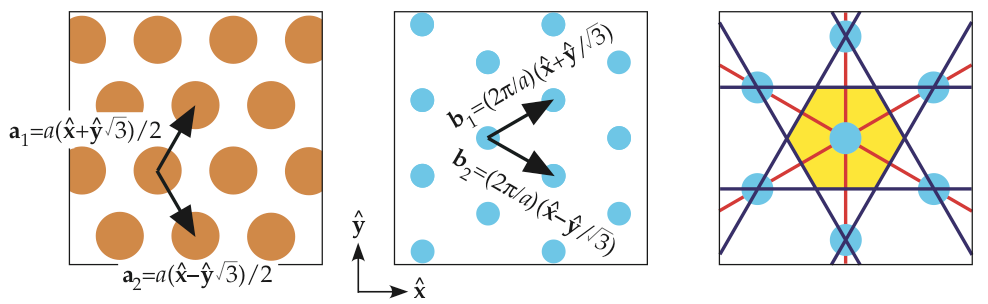
\includegraphics[width=0.8\textwidth]{imgs/bzonehex.png}
\caption{\label{fig:bzonehex} On the left is the lattice points in real space.
    In the middle is the corresponding reciprocal lattice. On the right is the
    construction of the first Brillouin zone: straight lines are drawn from the
    origin to the other lattice points (red), their perpendicular bisectors are
    the Bragg planes (blue), and the innermost region enclosed by the Bragg
    planes is the first Brilloin zone (yellow). Image and caption adapted from
    source.\cite{MITnp}}
\end{figure}
%TODO: Explain image equations?

\begin{figure}[!h]
\centering
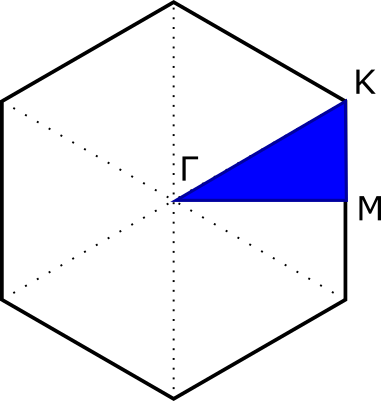
\includegraphics[width=0.3\textwidth]{imgs/hexibz.png}
\caption{\label{fig:ibzonehex} The irreducible Brillouin zone of the 2d
    hexagonal lattice in reciprocal space (blue).}
\end{figure}

Now as before, we can solve the dispersion relation over our infinite lattice
by just solving it over the boundary of the irreducible Brillouin as shown in
Figure~\ref{fig:ibzonehex}. First, let us find the values of $\kappa_{x}$ and
$\kappa_{y}$ at $\Gamma$, $K$ and $M$ as shown in the figure. We take
$\Gamma=(0,0)$ since it is the origin. 
%TODO: How to get K and M?

With this, and taking $M_i=k=\tilde{k}=1$ for simplicity, we get the dispersion
relation in Figure~\ref{fig:hexdisper}.

\begin{figure}[!h]
\centering
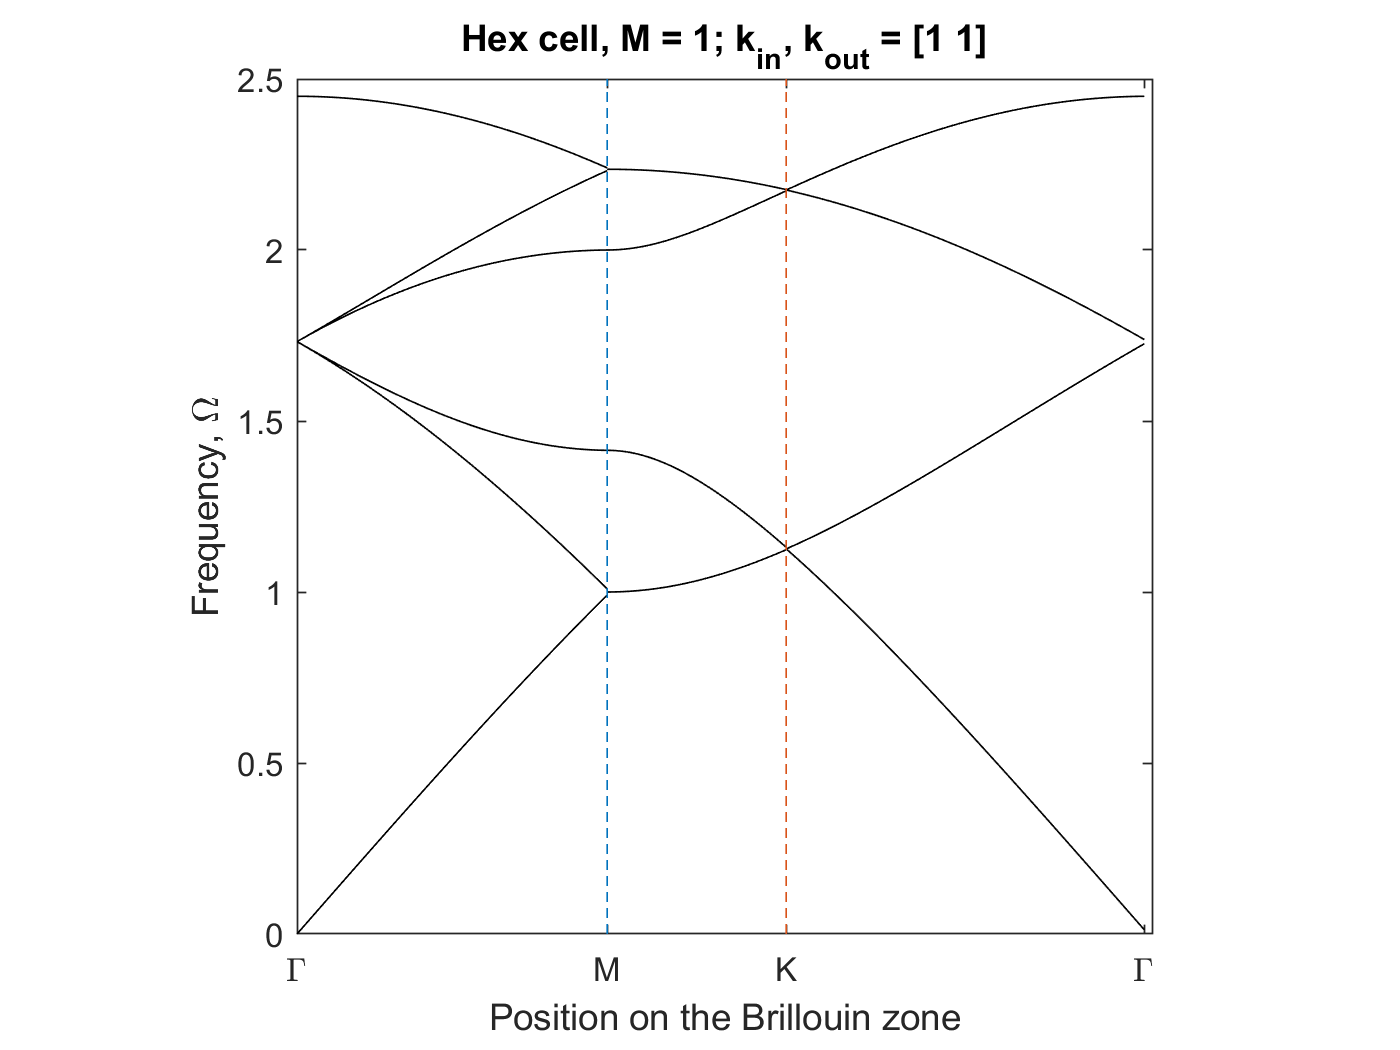
\includegraphics[width=0.8\textwidth]{imgs/hexdisper.png}
\caption{\label{fig:hexdisper} The dispersion relation of the 2d hexagonal
    lattice with $M_i=k=\tilde{k}=1$.}
\end{figure}

%TODO: Complete discussion of hex dispersion relation

\section{2d kagome lattice}
We will now investigate the kagome lattice, which is also known as the
trihexagonal tiling as it consists of triangles surrounding hexagons, as shown
in Figure~\ref{fig:kagomescheme}.

\begin{figure}[!h]
\centering
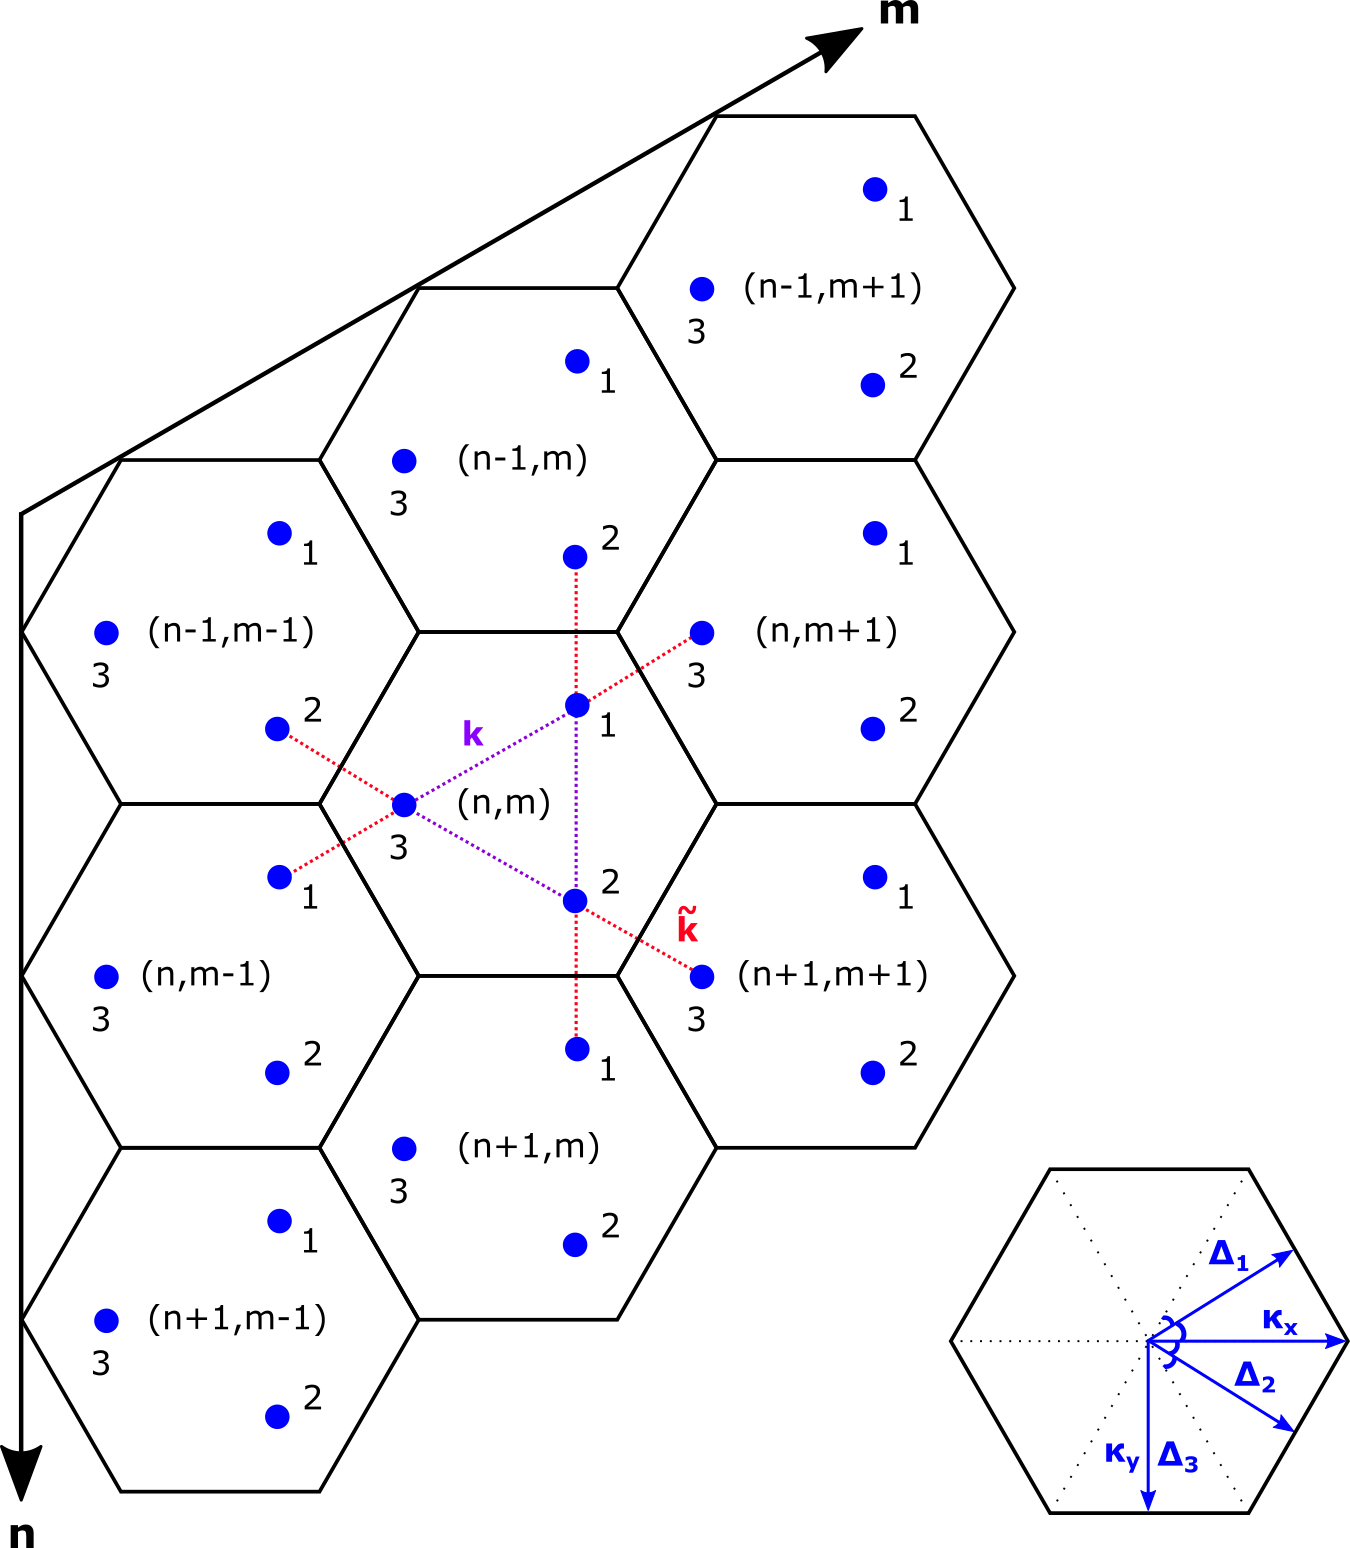
\includegraphics[width=0.8\textwidth]{imgs/kagomemodel.png}
\caption{\label{fig:kagomescheme} Schematic view of our 2d kagome model. Each
  hexagonal tile in the grid corresponds to one elementary cell with three
  masses. $k$ and $\tilde{k}$ represent the intra- and inter-cell spring
  constants respectively. The cell in the far bottom right shows the directions
  of the Bloch phases. Note that only the elastic interactions involving the
  masses in cell $(n,m)$ are shown to avoid cluttering the figure, although
  they exist within and between each cell.}
\end{figure}

Now again playing the same game as before, we can construct second order
differential equations which couple the displacements of connected masses. For
example, considering $M_1^{n,m}$, we get

\begin{align}
  F_1=M_1\frac{d^{2}}{dt^{2}}y_1^{n,m}
      =k\left(y_2^{n,m}+y_3^{n,m}-2y_1^{n,m}\right)+
       \tilde{k}\left(y_2^{n-1,m}+y_3^{n,m+1}-2y_1^{n,m}\right)
\label{eq:2dK1}
\end{align}

Due to the similarities in the shape of the elementary cell of the kagome
lattice and the hexagonal lattice, the Bloch phases are the same and we can
reuse \eqref{eq:hexvec1}, \eqref{eq:hexvec2} and \eqref{eq:hexvec3} as lattice
vectors. In doing so, we find the following relationships:

\begin{equation}
  y_1^{n+1,m}=e^{i\Delta_3}y_1^{n,m}
\label{eq:kagomerelate1a}
\end{equation}

\begin{equation}
  y_1^{n,m-1}=e^{-i\Delta_1}y_1^{n,m}
\label{eq:kagomerelate1b}
\end{equation}

\begin{equation}
  y_2^{n-1,m}=e^{-i\Delta_3}y_2^{n,m}
\label{eq:kagomerelate2a}
\end{equation}

\begin{equation}
  y_2^{n-1,m-1}=e^{-i\Delta_2}y_2^{n,m}
\label{eq:kagomerelate2b}
\end{equation}

\begin{equation}
  y_3^{n,m+1}=e^{i\Delta_1}y_3^{n,m}
\label{eq:kagomerelate3a}
\end{equation}

\begin{equation}
  y_3^{n+1,m+1}=e^{i\Delta_2}y_3^{n,m}
\label{eq:kagomerelate3b}
\end{equation}

With these, and assuming we have a Bloch wave solution as described in
\eqref{eq:wavesol}, we can rewrite \eqref{eq:2dK1} as

\begin{align}
M_1\Omega_1^{2}y_1
      &=\left(2k+2\tilde{k}\right)y_1+\left(-k-\tilde{k}e^{-i\Delta_3}\right)y_2+\left(-k-\tilde{k}e^{i\Delta_1}\right)y_3
\label{eq:2dK2}
\end{align}

Again, by forming these equations for each of the three masses, and then
combining them into one matrix equation, we get the following eigen-problem.

\begin{align}
  \left[\matr{A}\left(\kappa_{x},\kappa_{y}\right)-\matr{\Omega}\matr{M}\right]\vec{y}=\vec{0}
\label{eq:kagomeeig}
\end{align}

where $\matr{\Omega}=\diag\left(\left\{\Omega_i^2\right\}\right)$,
$\matr{M}=\diag\left(\left\{M_i\right\}\right)$,
$\vec{y}=\left[\left\{y_i\right\}\right]^T$ and now

\begin{align}
  \matr{A}\left(\kappa_{x},\kappa_{y}\right)=\left[
\begin{array}{ccc}
2k+2\tilde{k} & -k-\tilde{k}e^{-i\Delta_3} & -k-\tilde{k}e^{i\Delta_1} \\
-k-\tilde{k}e^{i\Delta_3} & 2k+2\tilde{k} & -k-\tilde{k}e^{i\Delta_2} \\
-k-\tilde{k}e^{-i\Delta_1} & -k-\tilde{k}e^{-i\Delta_2} & 2k+2\tilde{k} 
\end{array}\right]
\end{align}

%TODO: Form equations up till eigenproblem

Again given the similarities between the kagome and hexagonal lattice, the
irreducible Brillouin zones happen to be identical as seen in
Figure~\ref{fig:ibzonekagome}.

\begin{figure}[!h]
\centering
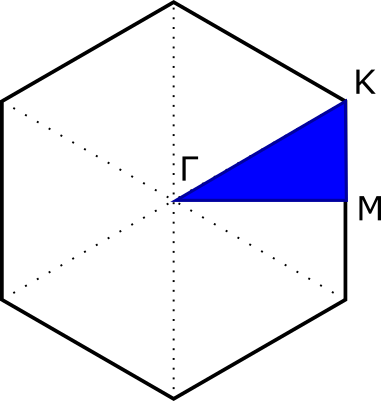
\includegraphics[width=0.3\textwidth]{imgs/kagomeibz.png}
\caption{\label{fig:ibzonekagome} The irreducible Brillouin zone of the 2d
    kagome lattice in reciprocal space (blue).}
\end{figure}

By solving this eigen-problem along the boundaries of the irreducible Brillouin
zone shown, we get the dispersion relation in Figure~\ref{fig:kagomedisper}.

\begin{figure}[!h]
\centering
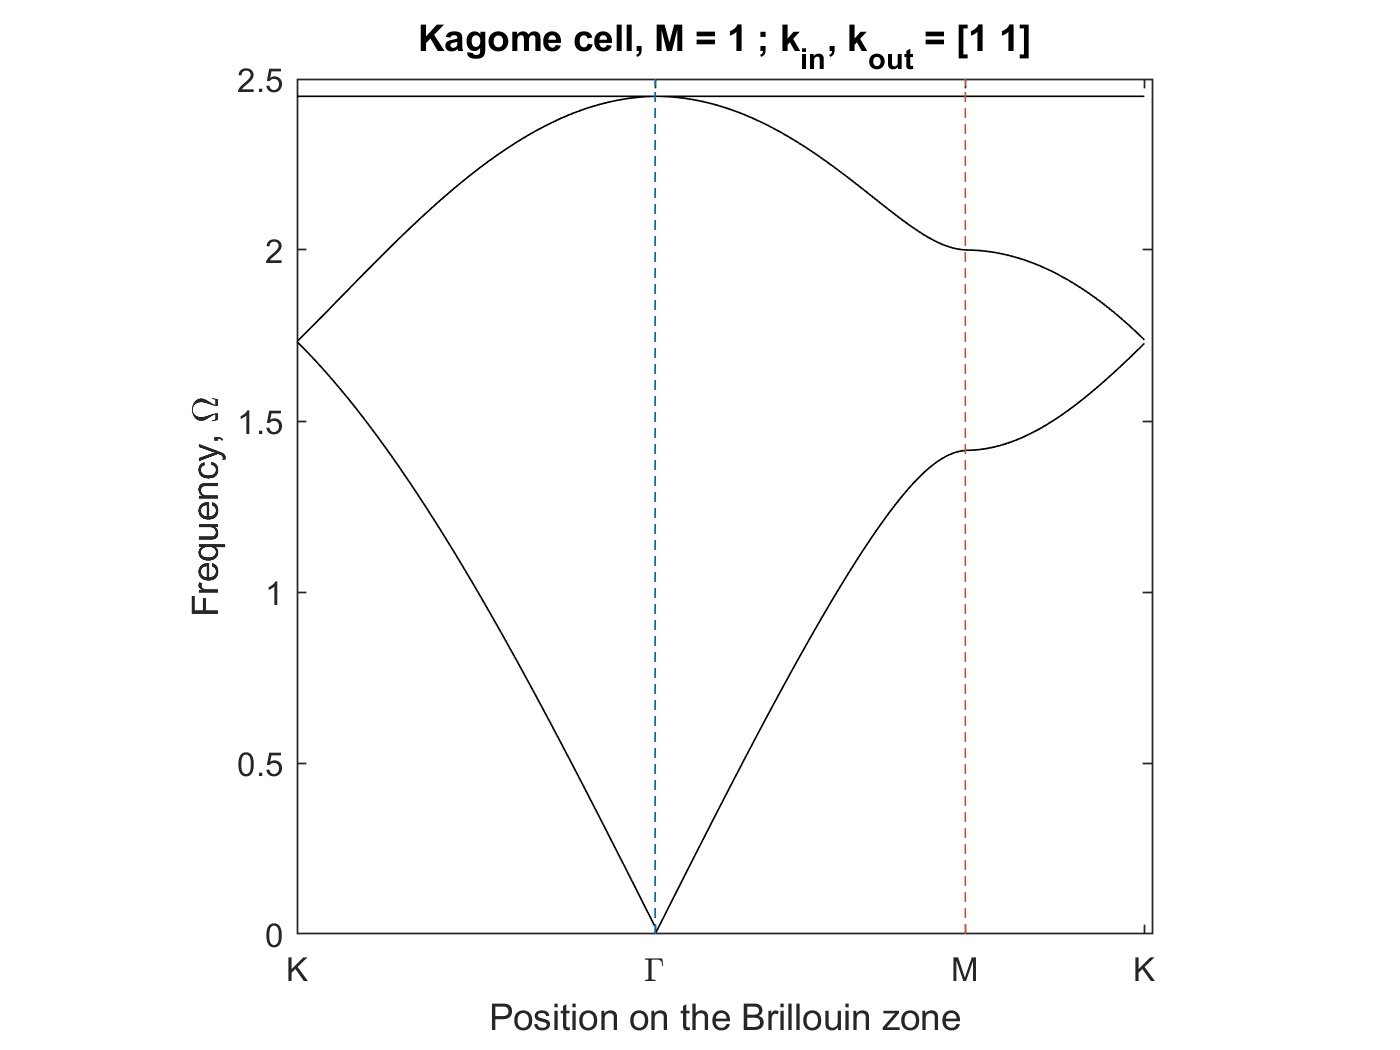
\includegraphics[width=0.8\textwidth]{imgs/kagomedisper.png}
\caption{\label{fig:kagomedisper} The dispersion relation of the 2d kagome
    lattice with $M_i=k=\tilde{k}=1$.}
\end{figure}

What is really interesting about this dispersion relation is that there is one
eigenvalue solution which is constant over the boundary of the irreducible
Brillouin zone; but not only that, it is actually constant over the entire
space!
%TODO: Explain why there is a flat line in kagome dispersion relation
%TODO: Explain significance of dispersion relation

\chapter{Perturbed system}
\label{perturbed}

So far, we have seen how to compute the dispersion relation for some simple
lattices. Now we want to see what sorts of effects we can create by introducing
some perturbations. We will do this in terms of changing the masses as well as
the spring constants between each mass in Chapter \ref{formbandgap}. Later on
in Chapter \ref{formstrip}, we will form a 2d strip or ribbon of these cells,
with the top half possessing one set of properties and the bottom half
possessing a different set of properties. We will see that this cause an
interesting phenomenon to occur at the boundary of the two halves.

\textit{Note}: As the hexagonal and kagome lattices contain more symmetries due
to the shape of their elementary cell, we will be focusing on perturbing these
models, but the same can be done for the square lattice as well. 

\section{Band gap}
\label{formbandgap}

\begin{figure}[!h]
\centering
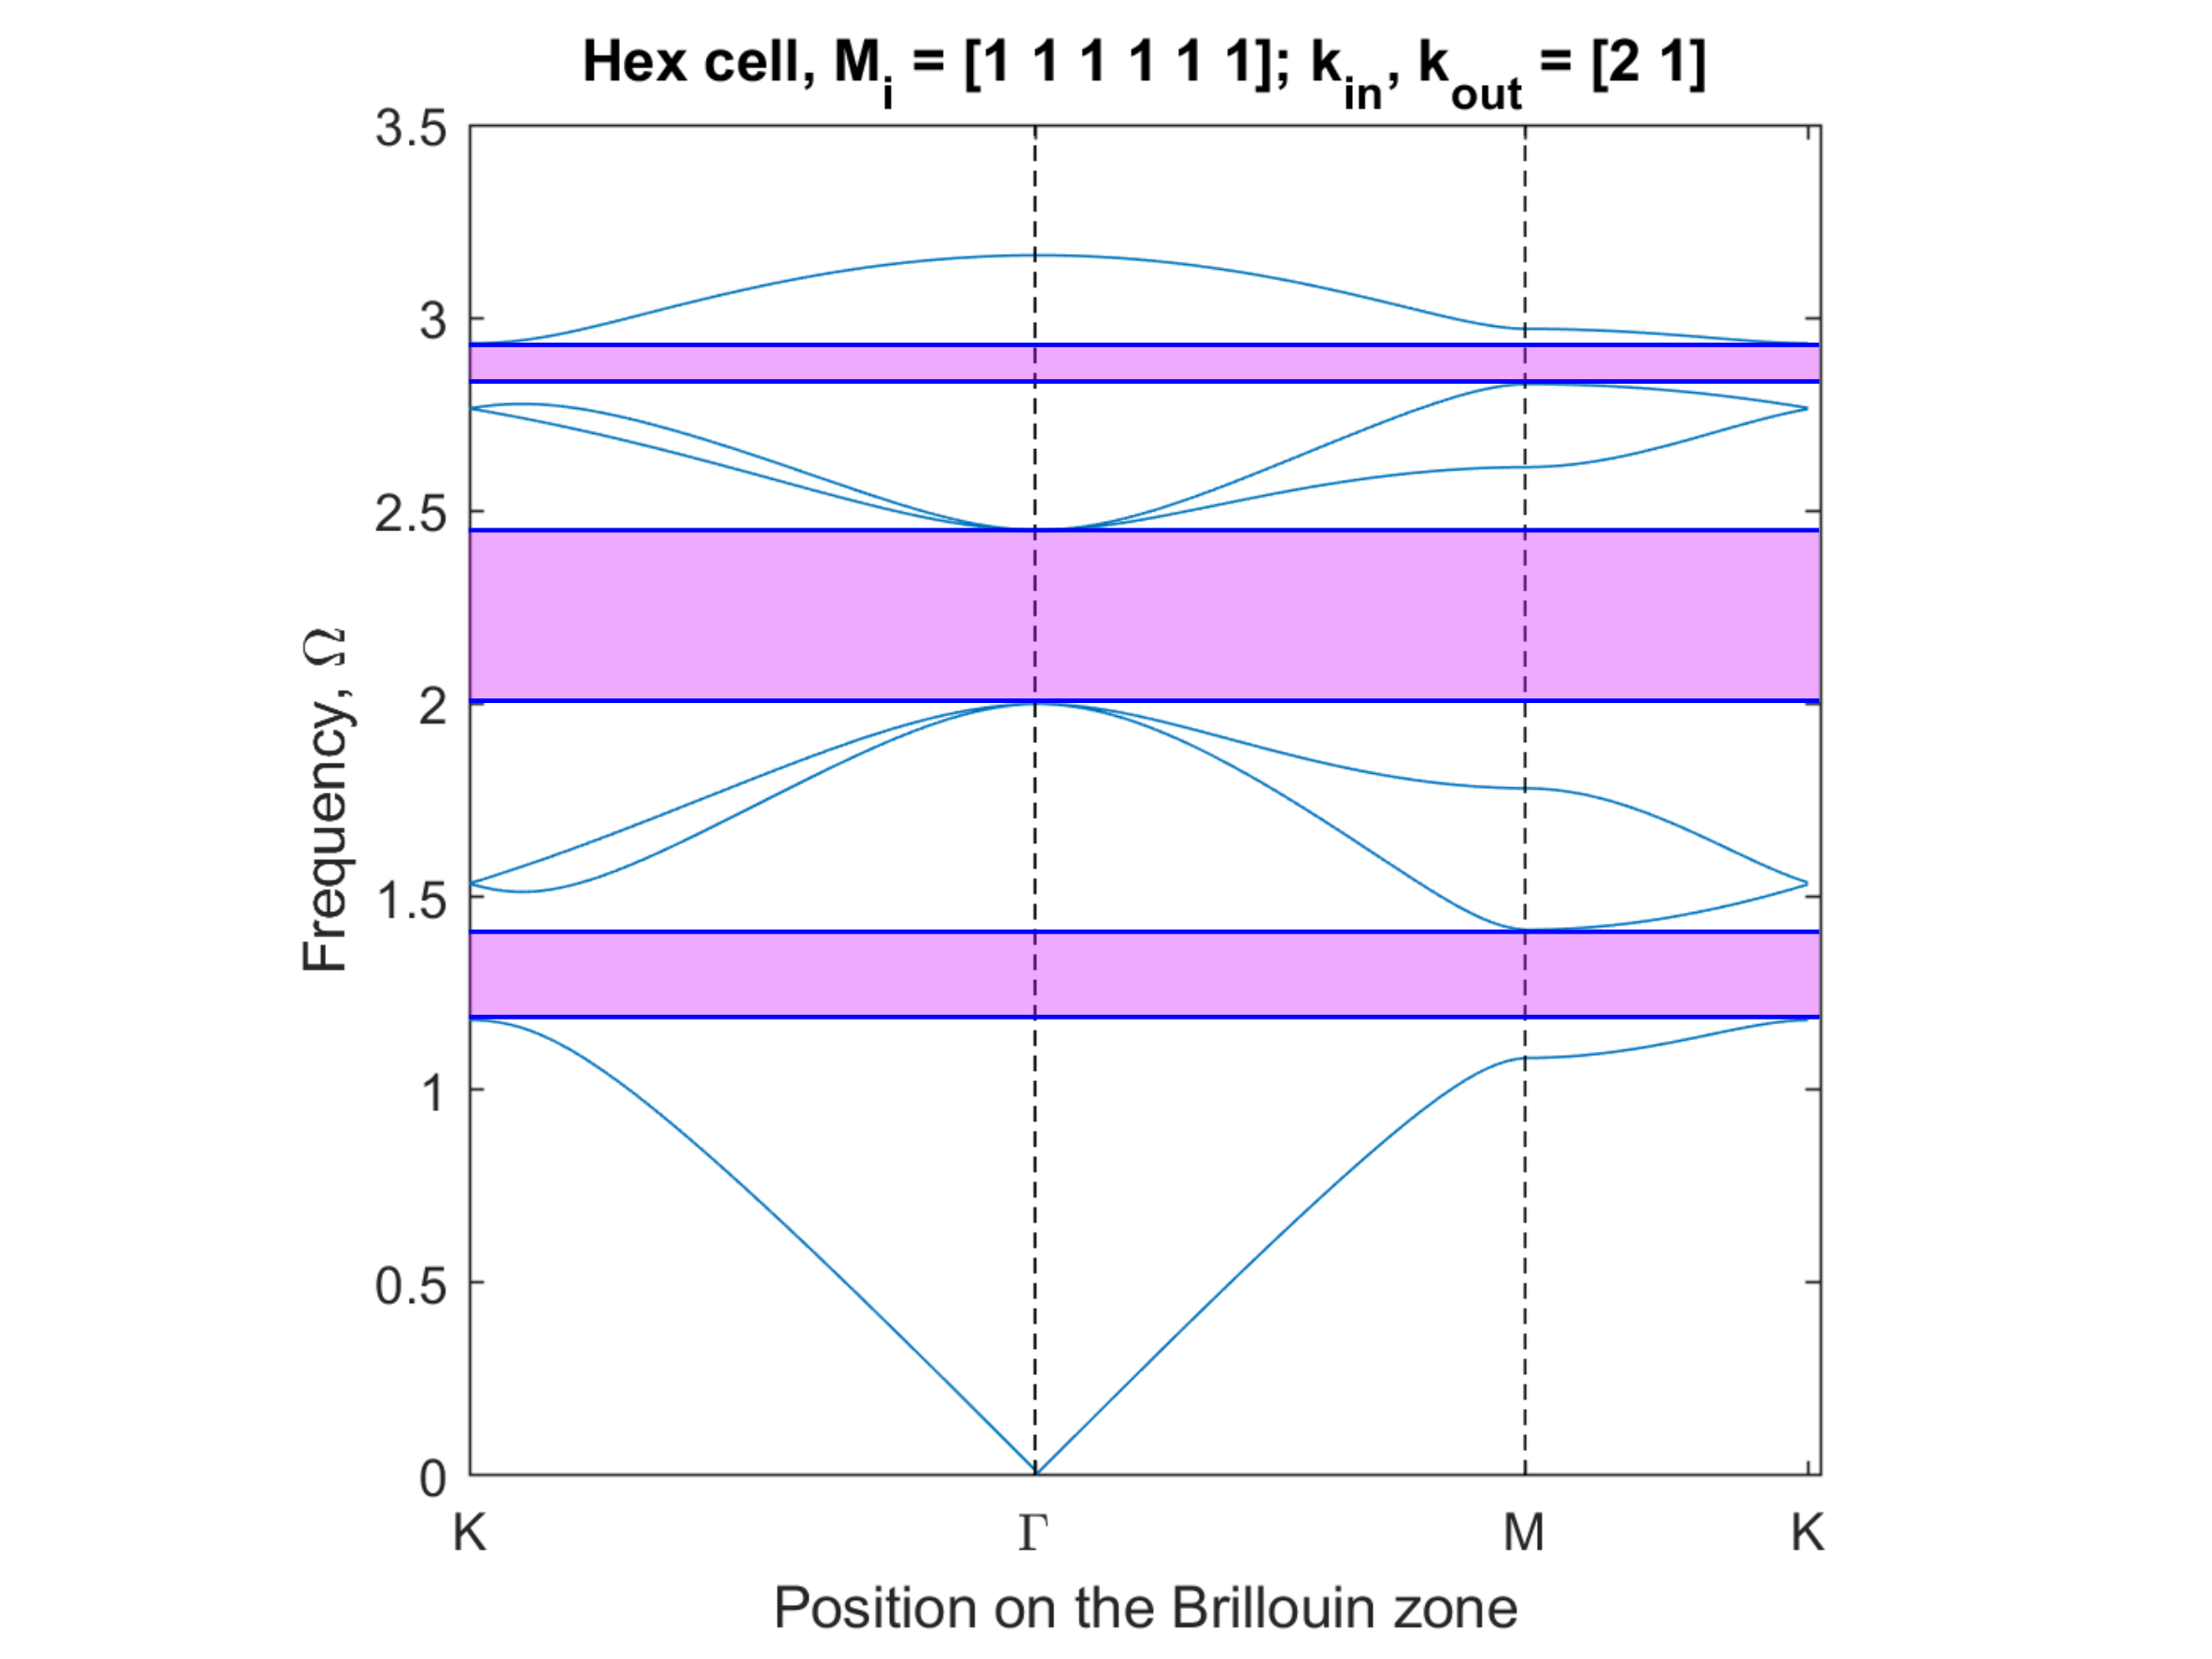
\includegraphics[width=0.8\textwidth]{imgs/bandgapex.png}
\caption{\label{fig:bandgapex} Example of bandgap (purple) formed in dispersion
  relation of hex lattice when $k=2$ and $\tilde{k}=1$.}
\end{figure}

A band gap, also called an energy gap, is an energy range where no wave states
can exist. In terms of our lattices, this corresponds to a range of frequencies
where waves are unable to propagate through the material; and in graphs of
dispersion relations, it is seen as gaps in the frequency axis where no line
is present. An example is shown in Figure~\ref{fig:bandgapex}. Notice that the
bandgaps are formed by the Dirac points breaking apart.

\section{2d bulk hexagonal perturbation}
Due to the many symmetries of the hexagonal lattice, there are many different
ways for us to perturb its structure and break its symmetry. These all lead to
slightly different effects on the dispersion relation.

\subsection{Alternating masses}
One way to perturb our bulk hexagonal lattice is by breaking one of its
rotational symmetries. Currently our hexagonal lattice has six-fold rotational
symmetry, i.e. rotating our cells by $\frac{2\pi}{6}$ do not change them. We can
reduce this to a three-fold symmetry by alternating the masses such that
$M_1=M_3=M_5 \neq M_2=M_4=M_6$.

\begin{figure}[!h]
\centering
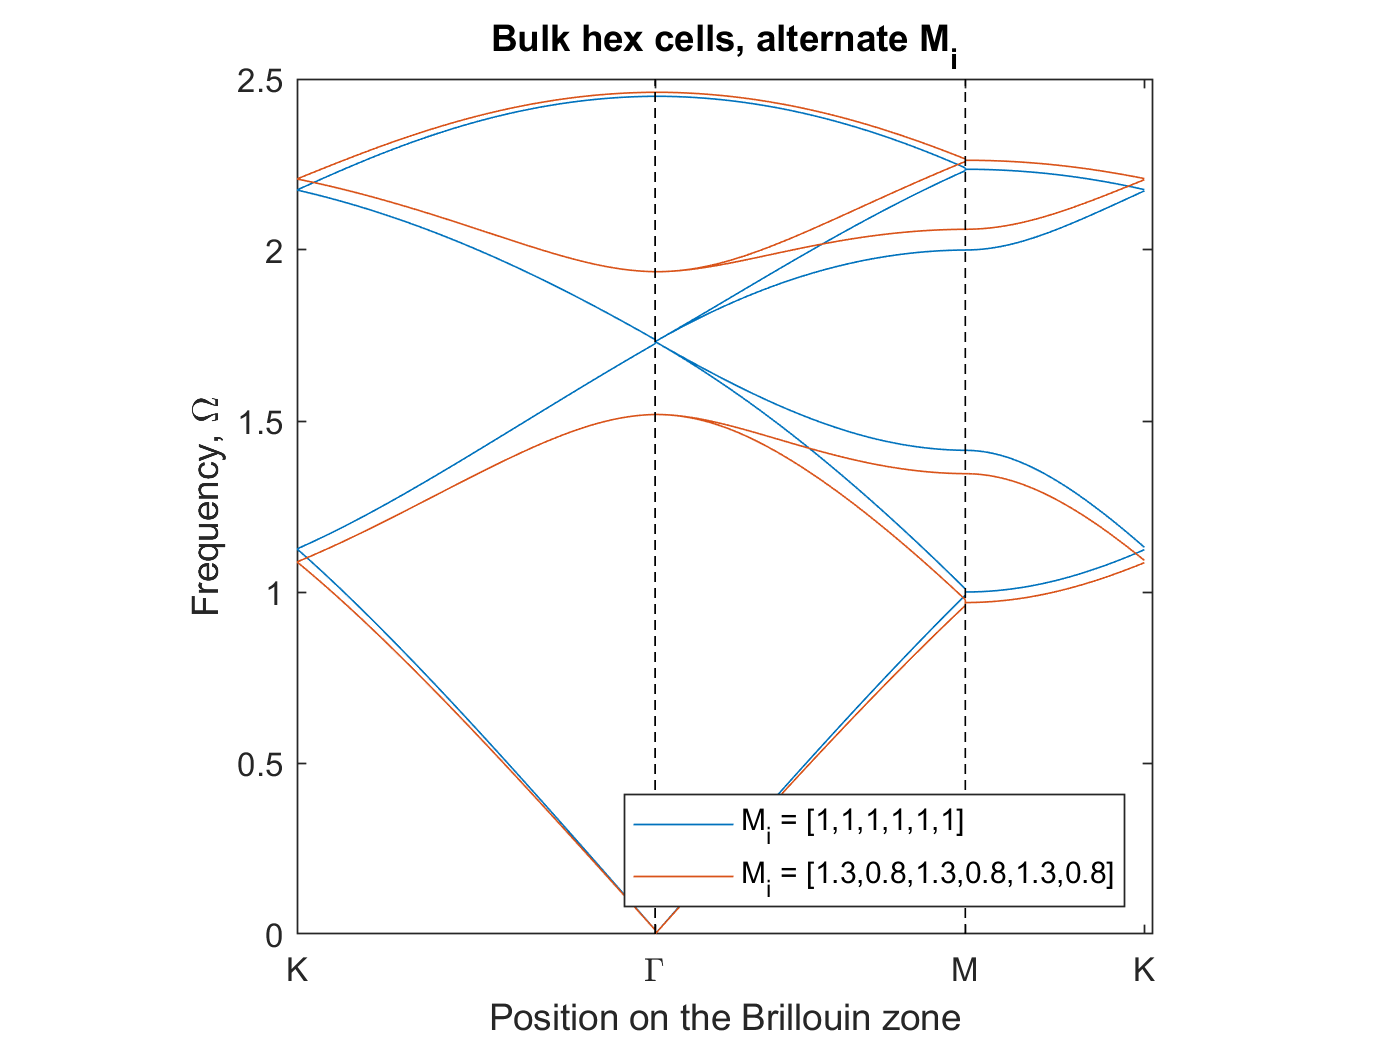
\includegraphics[width=0.8\textwidth]{imgs/hexperturbM.png}
\caption{\label{fig:hexM} The effect of alternating the masses $M_i$ on the
  dispersion relation of the bulk hexagonal system, with all other parameters
  set to $1$.}
\end{figure}

In Figure~\ref{fig:hexM}, we see that alternating masses has opened up the
Dirac point at $\Gamma$ and formed a bandgap.

\subsection{Varying mass and stiffnesses}
Another way we can induce a bandgap in our system is by changing the ratio of
the inner stiffness to the outer stiffness. This not only breaks one of the
local symmetries (local in the sense of the individual cell) but also breaks
one of the \textit{global} symmetries that we get. This perturbation is an
analogue to what is presented in this paper on photonic crystals.\cite{wuandhu}
This allows us to evaluate the validity and applicability of our system to
modelling more complex systems and is what we focus on in Chapter
\ref{reproduce}.

If you look at our hexagonal lattice and focus on the springs connecting our
masses, you can see that we have two different hexagons being formed, one
within each cell and also another between three adjacent cells meeting at a
vertex. When we have $k=\tilde{k}$, the inner and outer springs "tug" on the
masses the same amount, and so the two different hexagons we were talking about
before are of exactly the same proportions. However, when we modify our system
such that the inner stiffness is greater, say, than the outer stiffness, the
inner hexagons within each cell will be more "tightly pulled in" on itself and
in turn causing the outer hexagons to become bigger. This is shown in
Figure~\ref{fig:hextug}.

\begin{figure}[!h]
\begin{subfigure}[b]{.33\textwidth}
  \centering
  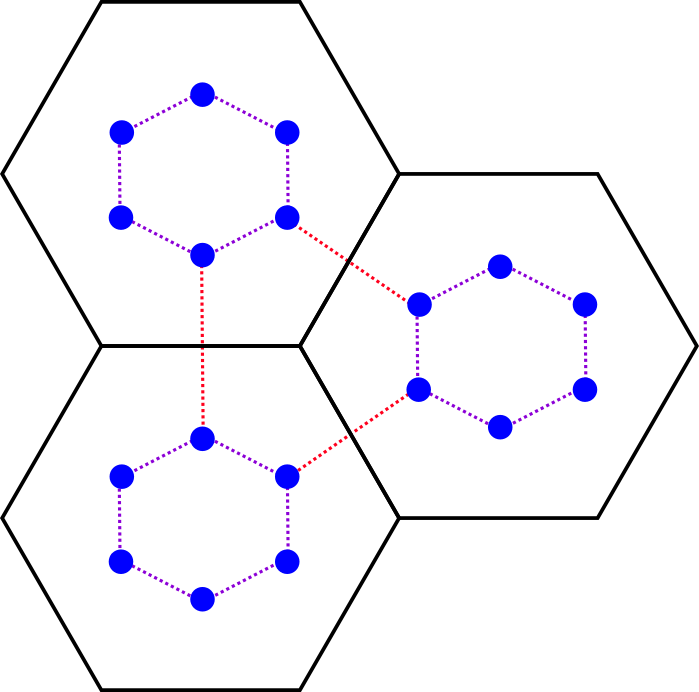
\includegraphics[width=1\linewidth]{imgs/hextugsmall.png}
  \caption{$k>\tilde{k}=1$}
\end{subfigure}%
\begin{subfigure}[b]{.33\textwidth}
  \centering
  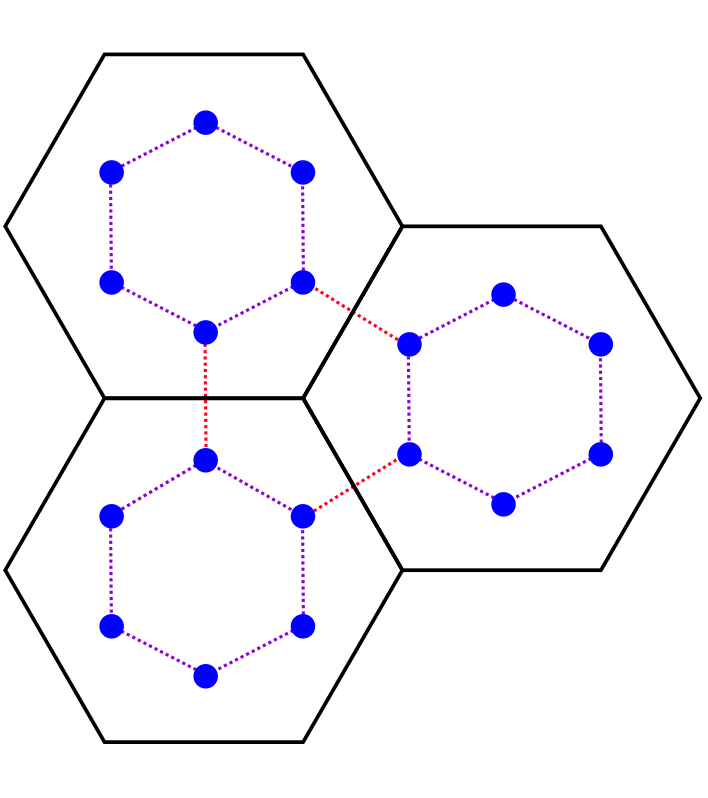
\includegraphics[width=1\linewidth]{imgs/hextug.png}
  \caption{$k=\tilde{k}=1$}
\end{subfigure}%
\begin{subfigure}[b]{.33\textwidth}
  \centering
  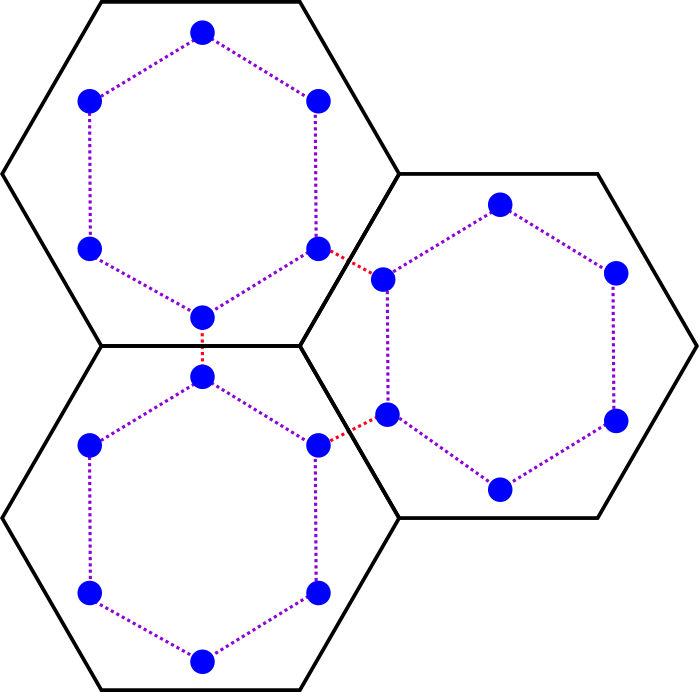
\includegraphics[width=1\linewidth]{imgs/hextugbig.png}
  \caption{$k<\tilde{k}=1$}
\end{subfigure}%
\caption{\label{fig:hextug} The effect of varying $k$ on the sizes of the inner
  and outer hexagons in the hexagonal lattice.}
\end{figure}

\begin{figure}[!h]
\centering
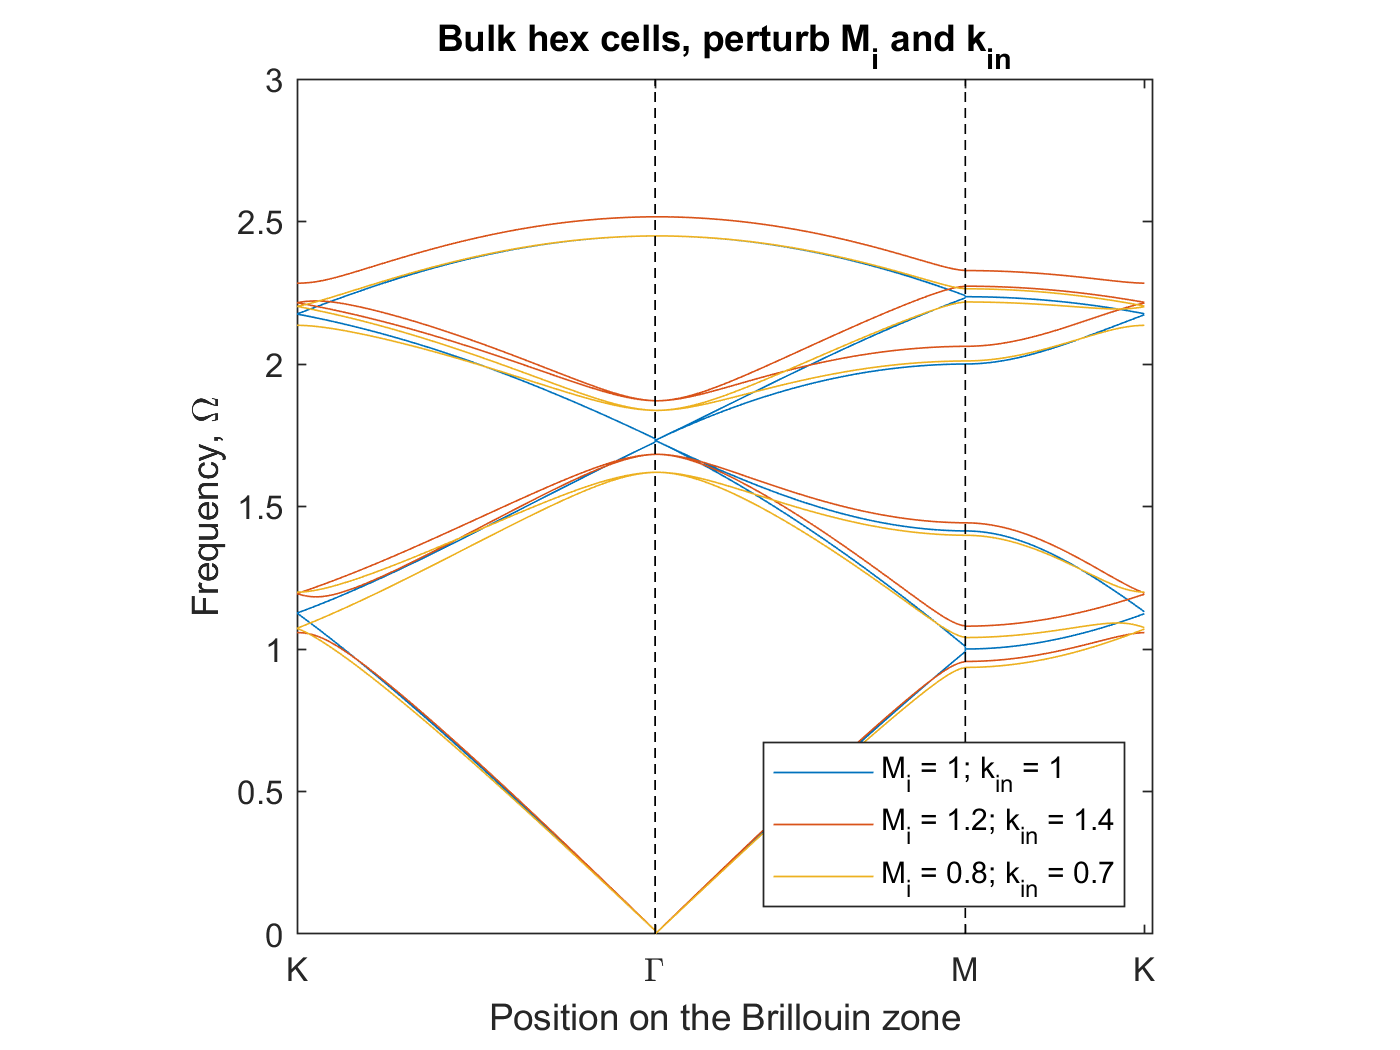
\includegraphics[width=0.8\textwidth]{imgs/hexperturb2.png}
\caption{\label{fig:hex2} The effect of perturbing the masses $M_i$ and
  $k$ on the dispersion relation of the bulk hexagonal system, with all other
  parameters set to $1$.}
\end{figure}

Very interestingly, we can see in Figure~\ref{fig:hex2} that increasing both
the mass and inner stiffness as well as decreasing both the mass and inner
stiffness leads to the formation of three bandgaps. This means that this time
we break all three Dirac points! We take a closer look at how changing $M_i$
and changing $k$ individually affect the dispersion relation in the kagome
lattice in Chapter \ref{kagomeperturb}.

\section{2d hexagonal strip}
\label{formstrip}
%TODO: How does bandgap relate to the dispersion along the boundary?

\begin{figure}[!h]
\centering
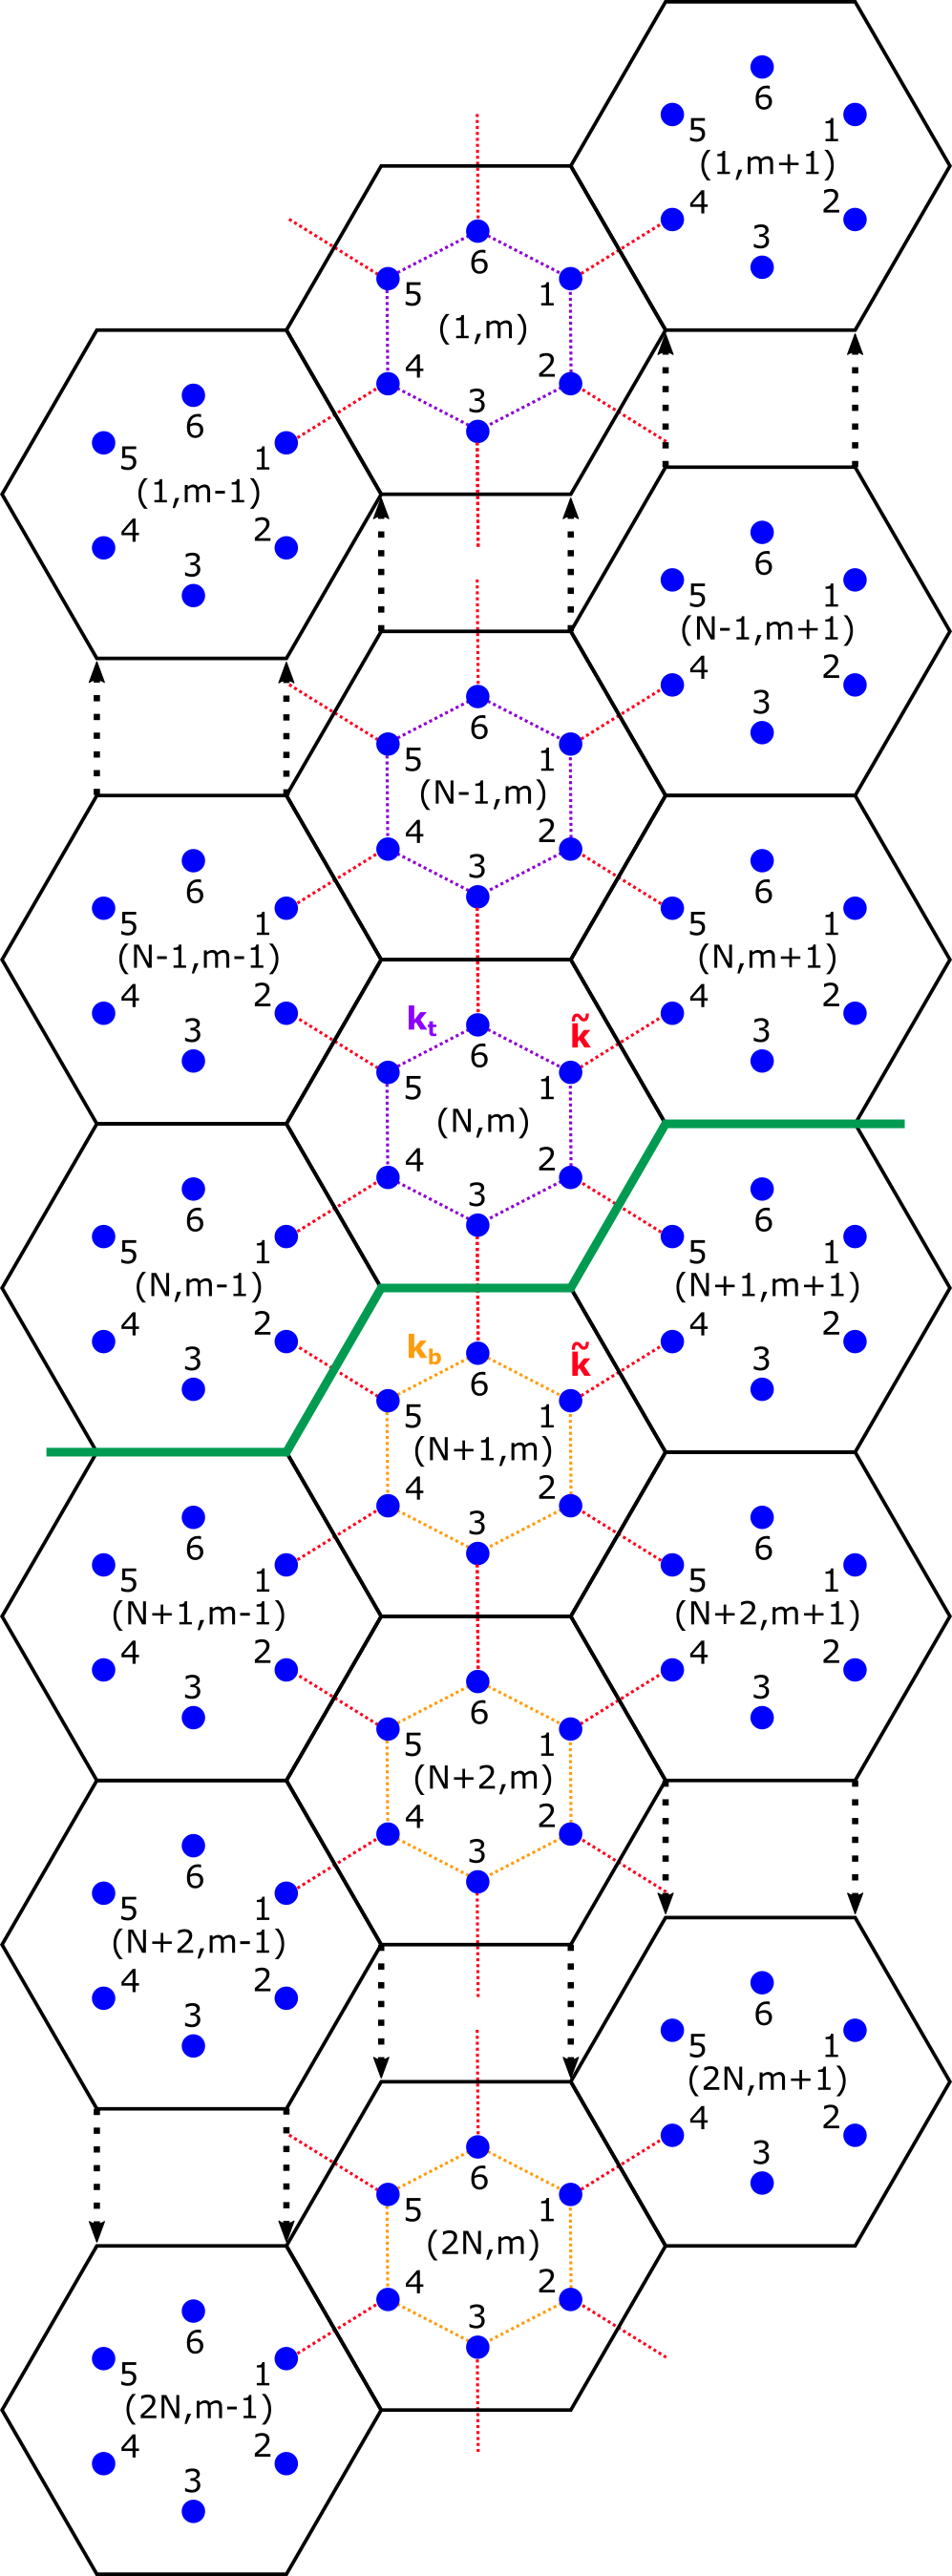
\includegraphics[width=0.4\textwidth]{imgs/hexstripmodel.png}
\caption{\label{fig:hexstripmodel} Schematic view of the 2d hexagonal
  semi-infinite lattice made from an infinite number of strips connected
  side-by-side. Each strip is composed of 2N cells, with the top half of cells
  above the boundary (green) possessing a set of properties and the bottom half
  possessing a separate set of properties. Note the the boundary conditions at
  the top and bottom, i.e. the cells at the top and bottom edges have no
  connections outside the lattice.}
\end{figure}

Now we assemble $2N$ hexagonal cells together into a strip and form a
semi-infinite hexagonal lattice by joining these strips from side-to-side as
shown in Figure~\ref{fig:hexstripmodel}. We will subscript the values
corresponding to the top half and bottom half with $t$ and $b$ respectively,
e.g. $k_t$ to refer to the inner spring constants for the top half and
$M_{1,b}$ to refer to the mass of mass $1$ in the bottom half. We set the outer
spring constant, $\tilde{k}_t=\tilde{k}_b=\tilde{k}$ to be the same throughout
the strip, to ensure that it agrees on both sides of the boundary or interface.

Using the same reasonings in Chapter \ref{2dhexdisper} to form equations
between adjacent cells, we can also form an eigen-problem as before (where the
size of our matrix is now $(2N \times 6) \times (2N \times 6)$ instead of $6
\times 6$). The only difference and extra care we have to take is to insert the
right coupling terms between masses in different cells, e.g. $M_3$ is not
connected to $M_6$ displaced by some phase shift anymore, but is connected to
$M_6$ in the cell below. 

Also, we explicitly choose the boundary condition where the top and bottom
cells have no connections outside the lattice. This is similar to having our
top and bottom edges connected to a \textit{rigid wall} as our waves are unable
to leave the lattice from those two edges. This is important to note as the
rigid boundary gives rise to a different dispersion curve at the top and bottom
boundaries which can lead to propagation of waves that we do not want, such as
in Figure~\ref{fig:kagomegentlebendscat}.

\textit{Note:} Another sensible periodic boundary condition which we could have
imposed at the top and bottom edges is by coupling the top and bottom cells
together across the edge. Specifically, we could impose

\begin{align}
  \matr{A}_{6,6(2N-1)+3}&=\matr{A}_{6(2N-1)+3,6}=-\tilde{k} \\
  \matr{A}_{5,6(2N-1)+2}&=-\tilde{k}e^{-i\Delta_1} \\
  \matr{A}_{6(2N-1)+2,5}&=-\tilde{k}e^{i\Delta_1} 
\end{align}

This essentially gives us an infinite lattice going from top to bottom, with
top and bottom materials alternating. Therefore essentially, the significant
difference which we will see between the two boundary conditions is that one
models the top and bottom edge as edges between our materials and a rigid wall,
and the other models the top and bottom edge as edges between our two
materials. However, we will see later on that this will not matter too much for
our scattering simulations as we will be exciting waves of frequencies in our
bandgaps. So if we take $N$ to be large enough, the exponential decay of the
wavefunctions across the strip is great enough to ensure our wave does not
propagate to the top and bottom edges anyways.

With that out of the way, we can finally form the eigen-problem

\begin{align}
  \left[\matr{A}\left(\kappa_{x},\kappa_{y}\right)-\matr{\Omega}\matr{M}\right]\vec{y}=\vec{0}
\label{eq:hexstripeig}
\end{align}

where $\matr{A}$ is a $(2N \times 6) \times (2N \times 6)$ matrix with
$\matr{A}$ as defined in \eqref{eq:hexeig} repeated along the diagonal and with
the additional coupling terms added,
$\matr{\Omega}=\diag\left(\left\{\Omega_i^2\right\}\right)$,
$\matr{M}_{t}=\diag\left(\left\{M_{i,t}\right\}\right)$,
$\matr{M}_{b}=\diag\left(\left\{M_{i,b}\right\}\right)$,
\begin{align}
\matr{M}=\left[
\begin{array}{cccccc}
\matr{M}_{t}\\
 & \ddots &  &  & 0\\
 &  & \matr{M}_{t}\\
 &  &  & \matr{M}_{b}\\
 & 0 &  &  & \ddots\\
 &  &  &  &  & \matr{M}_{b}
\end{array}\right],
\end{align}

\begin{align}
\vec{y}=\left[
\begin{array}{c}
y_1^{(1)}\\
\vdots\\
y_6^{(1)}\\
\vdots\\
y_1^{(2N)}\\
\vdots\\
y_6^{(2N)}\\
\end{array}\right],
\end{align}

Now with this eigen-problem, all we have left to do is figure out what the
irreducible Brillouin zone for our ribbon system is.

We go from $K'=(-\frac{sqrt{3}\pi}{4},-\frac{pi}{4})$ to $\Gamma=(0,0)$ to
$K=(\frac{sqrt{3}\pi}{4},\frac{pi}{4})$.
%TODO: Add derivation of IBZ for hexagonal ribbon system

Solving this with $M_{i,t}=M_{i,b}=k_t=k_b=\tilde{k}=1$ over the irreducible
Brilloun zone gives us the dispersion relation in
Figure~\ref{fig:hexstripdisper}, which corresponds to what we see in
Figure~\ref{fig:hexdisper} (if you take the graph from $K$ to $\Gamma$ and then
reflect it about the vertical at $\Gamma$).

\begin{figure}[!h]
\centering
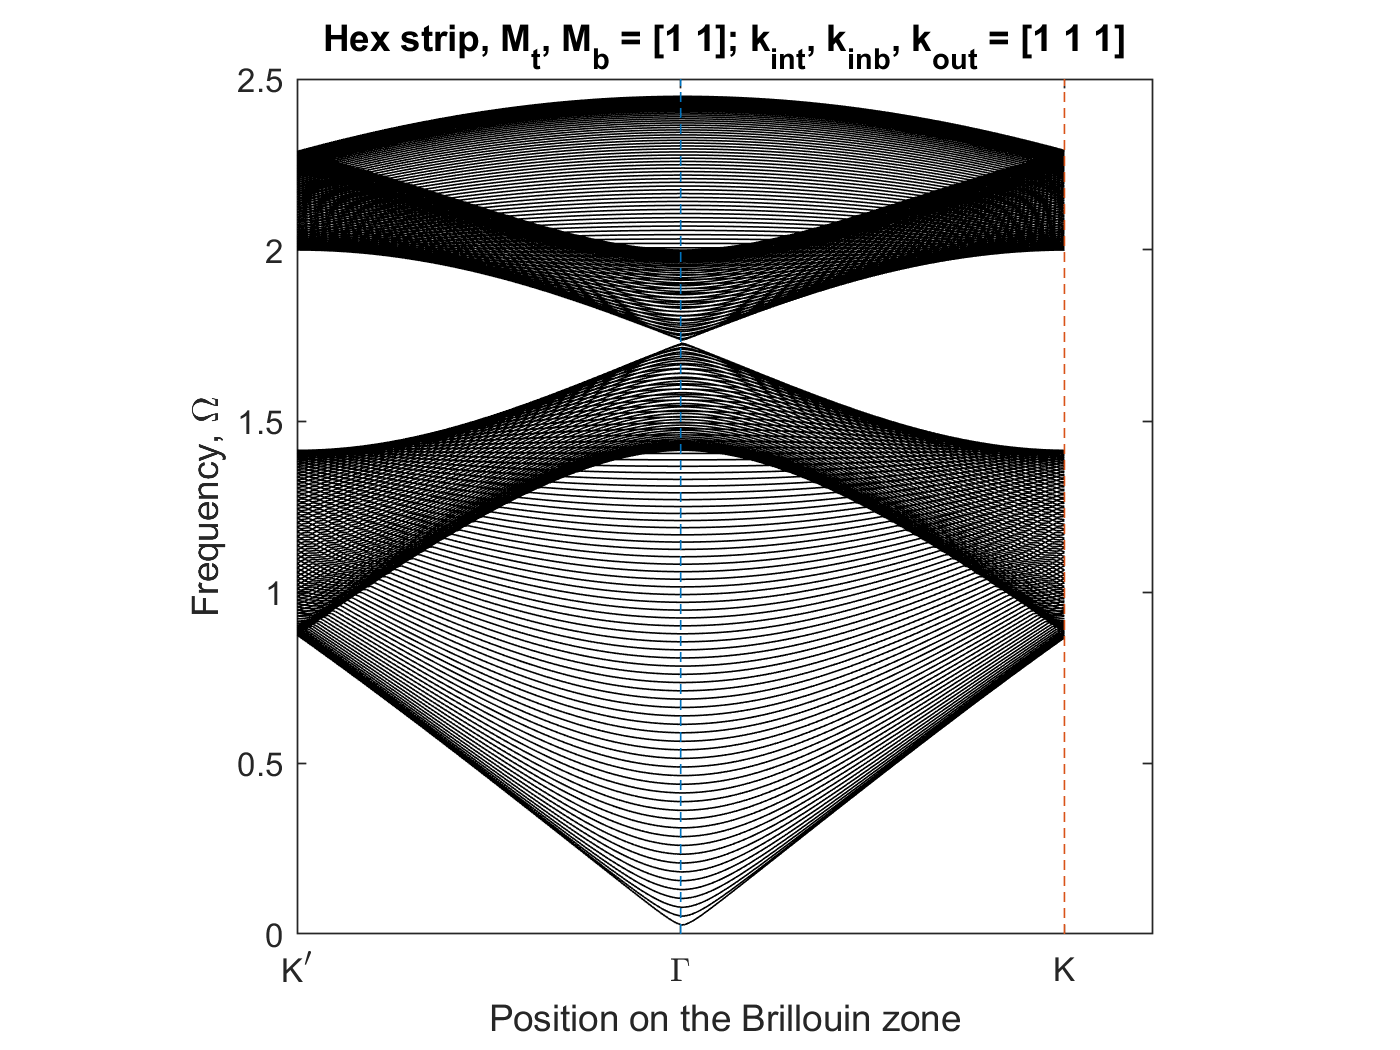
\includegraphics[width=0.8\textwidth]{imgs/hexstrip.png}
\caption{\label{fig:hexstripdisper} Dispersion relation of the semi-infinite
  hexagonal lattice with $2N=40$ (40 cells in total) with
  $M_{i,t}=M_{i,b}=k_t=k_b=\tilde{k}=1$.}
\end{figure}

As we have just done in Chapter \ref{formstrip}, we will see what happens to
the dispersion relation when we set the two layers of the lattice to have
different properties as those before which opened up a band gap.

\subsection{Alternating masses}
\label{perturbaltmass}
Using our results of the formation of a bandgap in, let us first see what
happens when we create a hexagonal strip where the top and bottom have the same
property of alternating masses. 

\begin{figure}[!h]
\centering
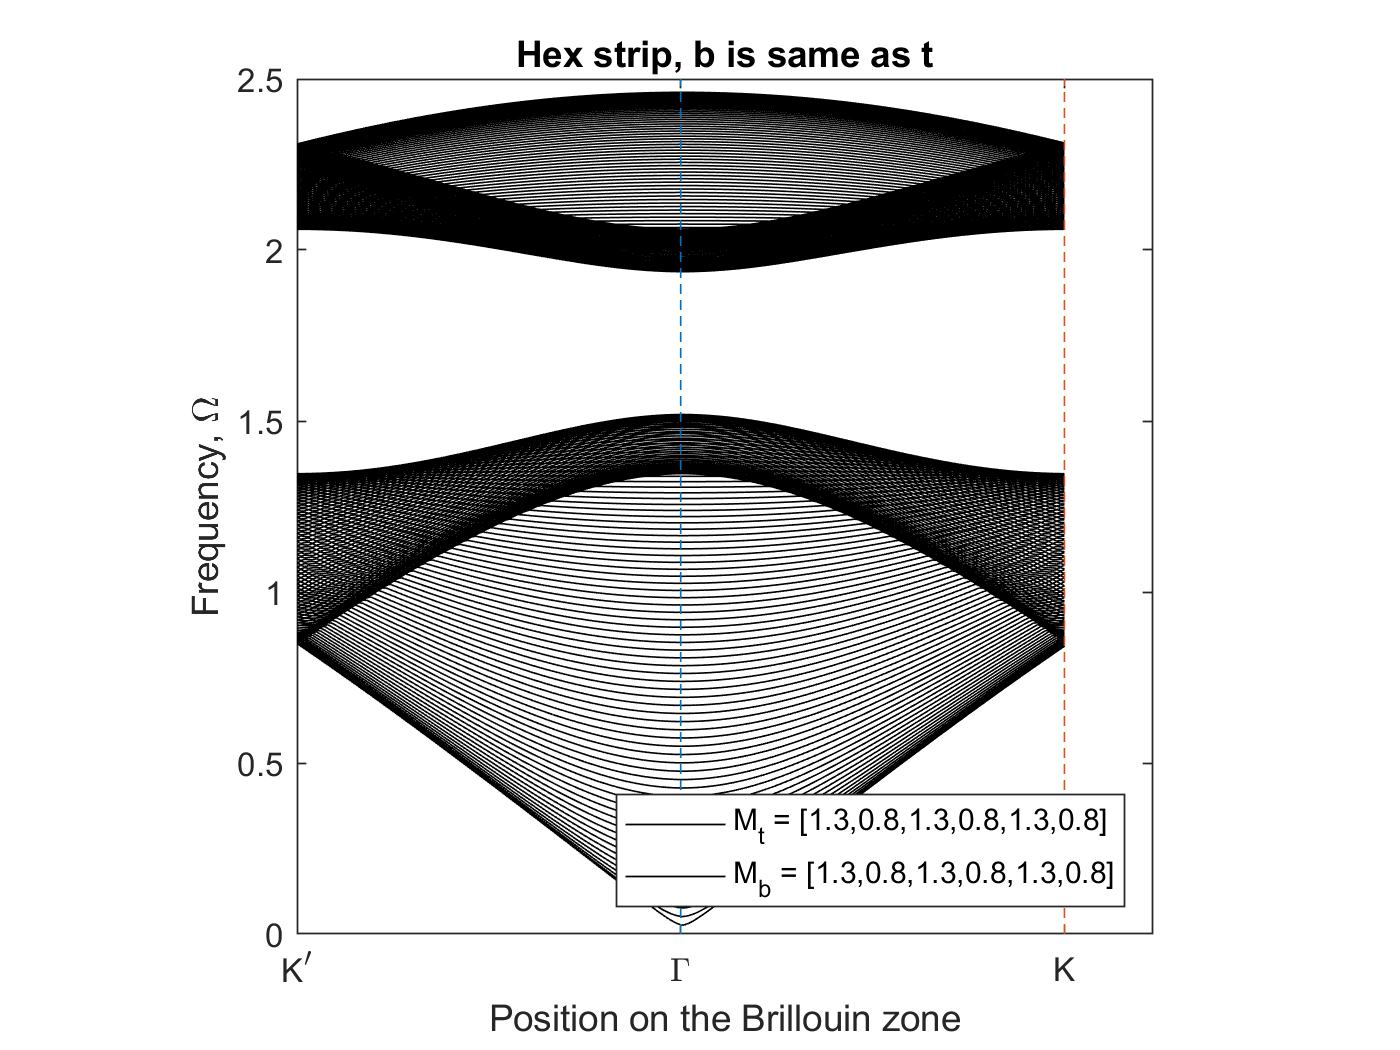
\includegraphics[width=0.8\textwidth]{imgs/hexstripperturbM.png}
\caption{\label{fig:hexstripM} Dispersion relation of the semi-infinite
  hexagonal lattice with alternating masses (with the top and bottom layer the
  same configuration), with all other parameters set to $1$.}
\end{figure}

Again, we see in Figure~\ref{fig:hexstripM} that basically the dispersion
relation we get corresponds to that of Figure~\ref{fig:hexM} (if you look at
the graph from $K$ to $\Gamma$ and reflect about $\Gamma$), where there is a
bandgap present. This is all fine and good but we can do something even better.

In this system, the two layers of materials are the same which means that
essentially it behaves just like the bulk hexagon case. It is as if we just
took a finite chunk of the infinite bulk lattice. So with that in mind, let us
change the bottom layer into a different configuration. The easiest way of
perturbing it so that we still get the exact same dispersion relation in the
bulk case is to rotate the cell by $\frac{2\pi}{6}$. This is because locally
(at the cellular level), nothing has changed and if we form a bulk system from
the rotated cell we still get the same bulk system but rotated, but this does
not affect the frequencies of waves allowed to propagate. So even if we stack
the two different types of cells on each other, we would expect the same
bandgap to be present, since locally each cell exhibits that property. However
if we now consider the global symmetry when stacking the two different
materials on top of each other, we can see that we have broken some sort of
translational symmetry and so would expect something different in the
dispersion relation.

\begin{figure}[!h]
\centering
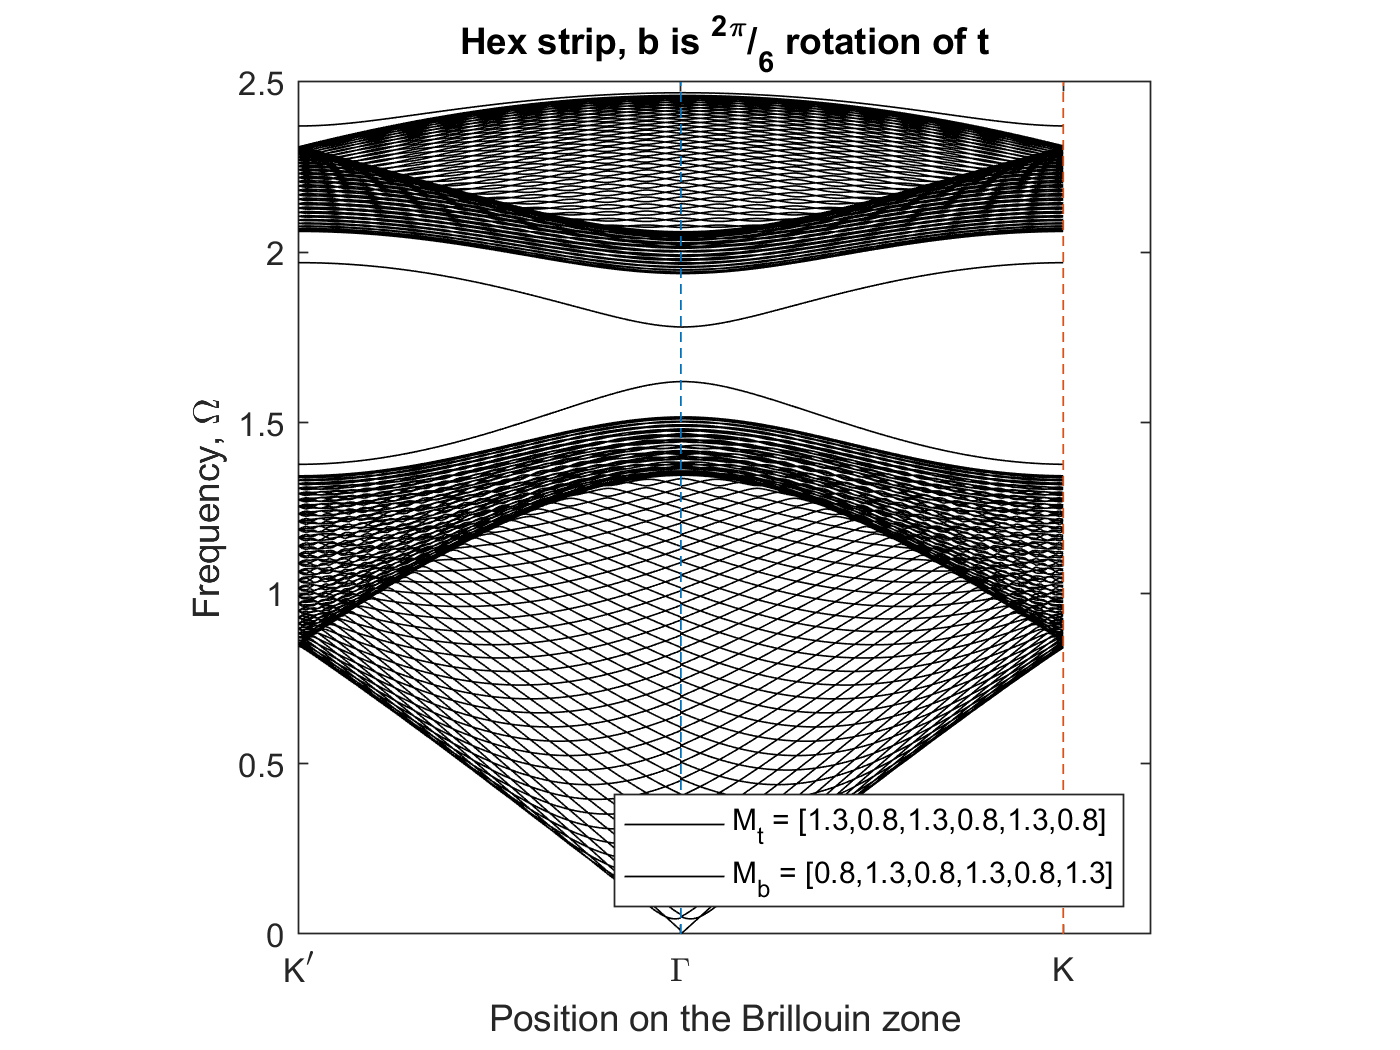
\includegraphics[width=0.8\textwidth]{imgs/hexstripperturbMrotated.png}
\caption{\label{fig:hexstripMrotated} Dispersion relation of the semi-infinite
  hexagonal lattice with alternating masses (with bottom layer as a
  $\frac{2\pi}{6}$ rotation of the top layer), with all other parameters set to
  $1$.}
\end{figure}

As expected, we see that in Figure~\ref{fig:hexstripMrotated} we get pretty
much the same dispersion relation as in Figure~\ref{fig:hexstripM} but with two
curious lines in the bandgap! This is really interesting and useful for us
because this means that all the frequencies along the two lines in the bandgap
are only able to propagate along the centre line of the semi-infinite lattice
we constructed, i.e. along the boundary and not anywhere else in the lattice.
The waves corresponding to the waves of these special frequencies are known as
the edge modes or edge states of our system, as they travel \textit{along the
edge} or boundary and exponentially decay outwards from that edge. With this
knowledge, we are then able to start trying to force energy to propagate in the
directions we desire in Chapter \ref{scattering}.
%TODO: How do we know it exponentially decays??
%TODO: Discuss the difference between the two lines, due to the periodic
%boundaries, one refers to the red over blue boundary, the other refers to blue
%over red

\subsection{Varying mass and stiffnesses}
\label{perturbMk}
We can do the same thing in this case, but instead of making the bottom layer a
rotation of the top layer, we make the top have a greater $M_i$ and $k$ and the
bottom have a lower $M_i$ and $k$. As we have seen in
Figure~\ref{fig:hex2}, we have one increased and one decreased system which
have similar bandgaps. As such, we will be using those two configurations to
form our strip.

\begin{figure}[!h]
\centering
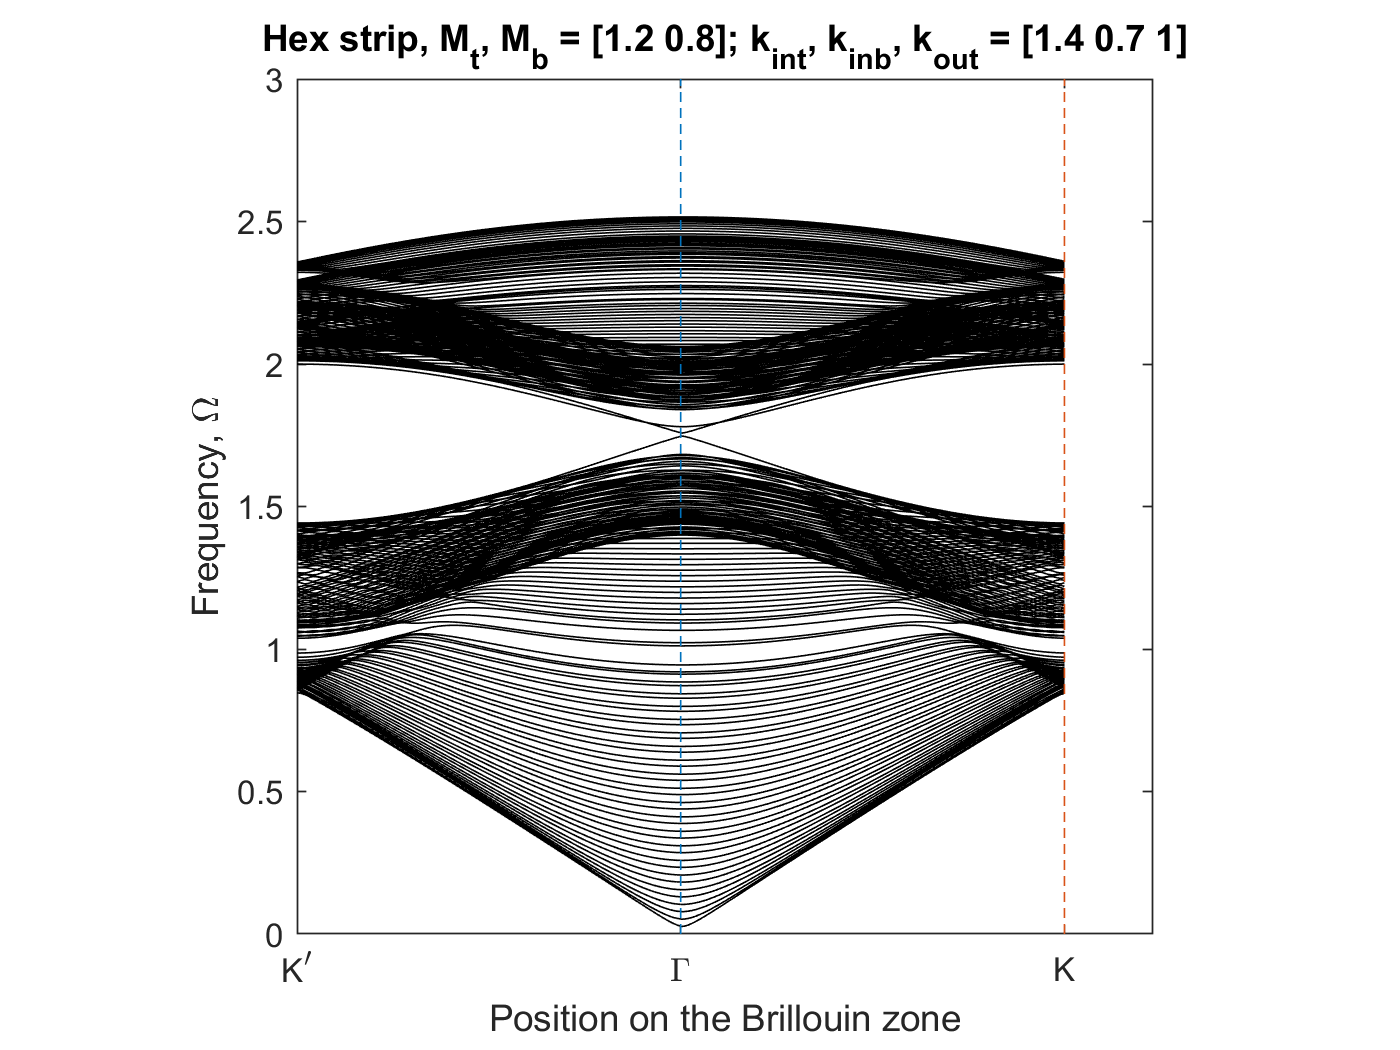
\includegraphics[width=0.8\textwidth]{imgs/hexstripperturb2.png}
\caption{\label{fig:hexstrip2} Dispersion relation of the semi-infinite
  hexagonal lattice where the top material has a higher $M_i$ and $k$ than the
  bottom material, with all other parameters set to $1$.}
\end{figure}

As before we again get a well-defined bandgap, as well as two dispersion lines
which are present in the bandgap and therefore correspond to edge states.

\section{2d bulk kagome perturbation}
\label{kagomeperturb}

Similarly to the hexagonal case, we can perturb the different parameters in our
bulk kagome system to see what effects they have on the dispersion relation.

\begin{figure}[!h]
\centering
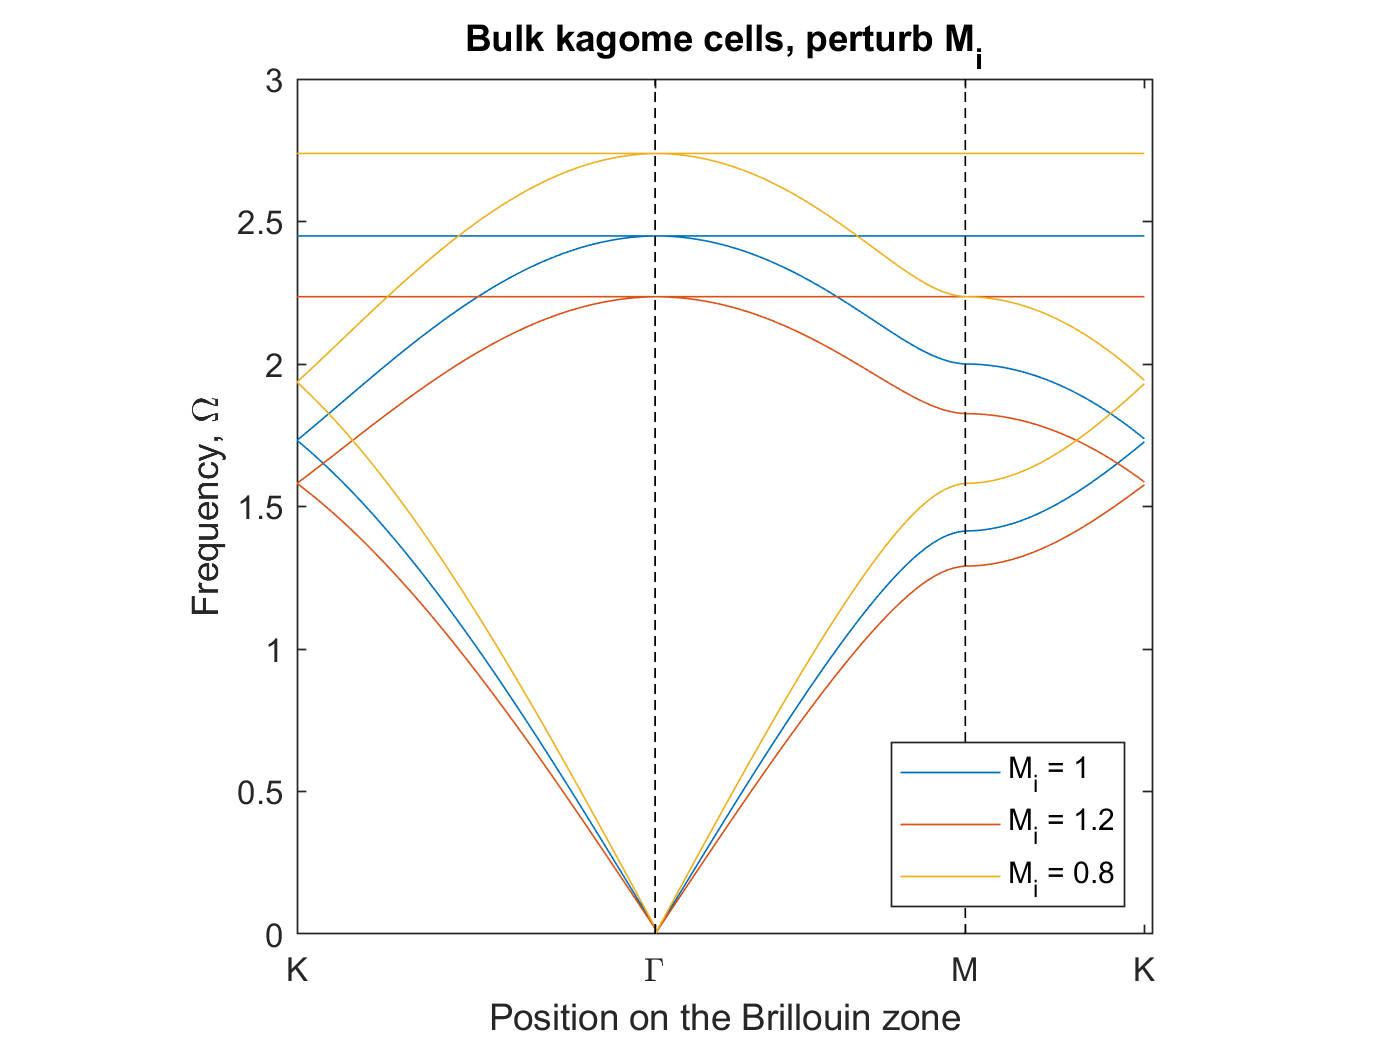
\includegraphics[width=0.8\textwidth]{imgs/kagomeperturbM.png}
\caption{\label{fig:kagomeM} The effect of perturbing the masses $M_i$ on the
  dispersion relation of the bulk kagome system, with all other parameters set
  to $1$.}
\end{figure}

\begin{figure}[!h]
\centering
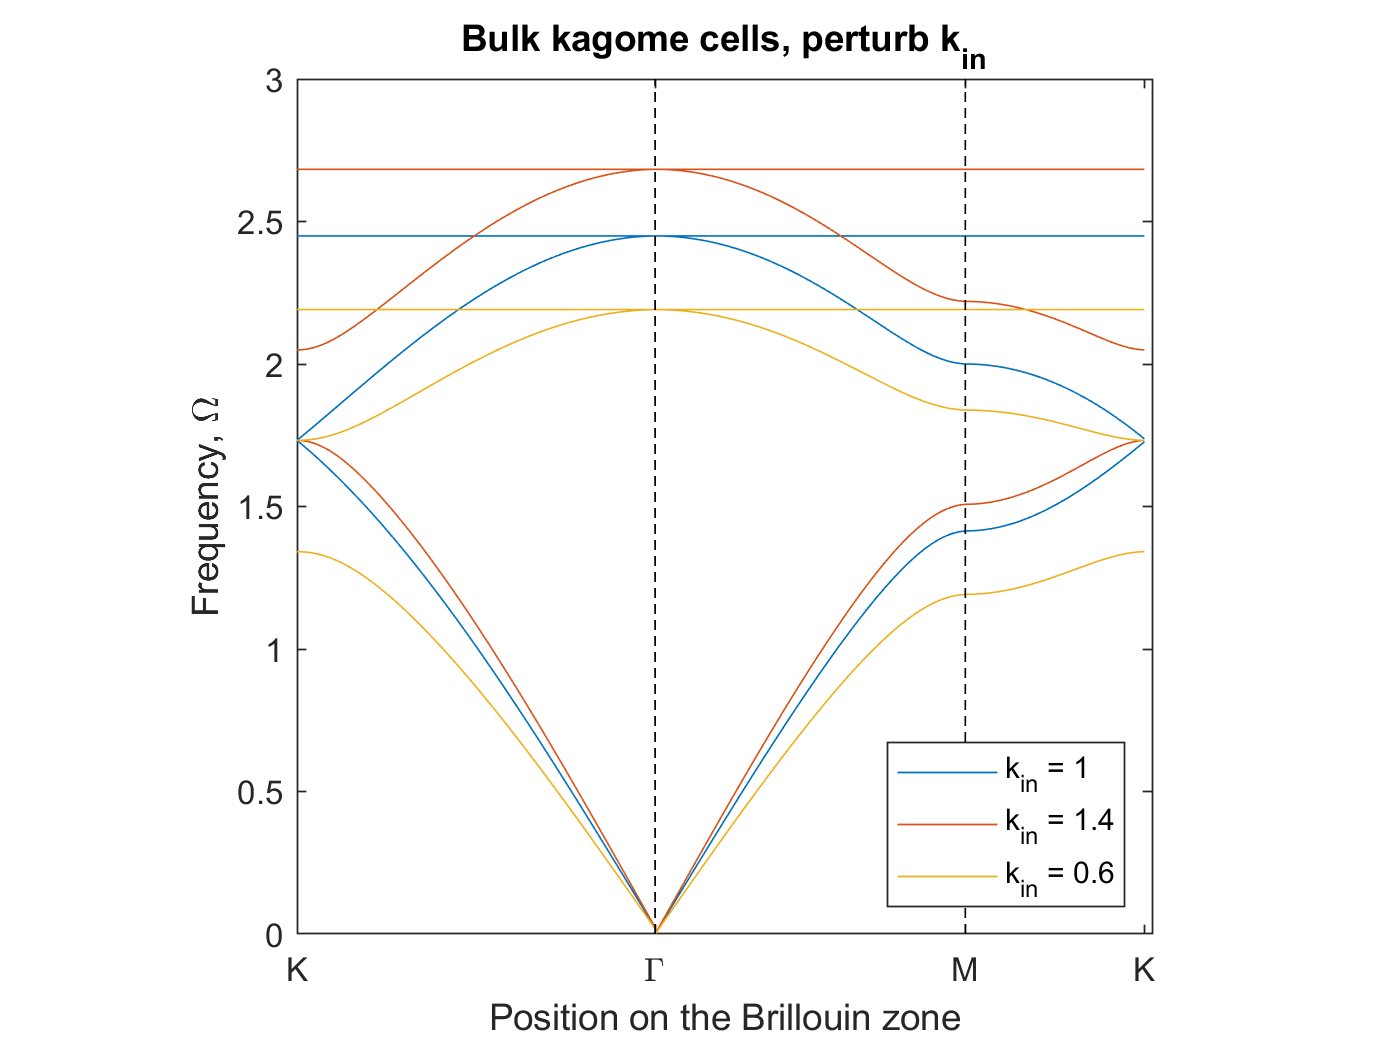
\includegraphics[width=0.8\textwidth]{imgs/kagomeperturbk.png}
\caption{\label{fig:kagomek} The effect of perturbing the inner stiffness $k$
  on the dispersion relation of the bulk kagome system, with all other
  parameters set to $1$.}
\end{figure}

We can see the effects that perturbing the masses $M_i$ and inner stiffness $k$
have on the bulk kagome system. In the case of varying $M_i$ in
Figure~\ref{fig:kagomeM}, increasing $M_i$ decreases or constrains the
dispersion relation, while decreasing $M_i$ increases or widens the dispersion
relation. 

However, in the case of varying $k$ in Figure~\ref{fig:kagomek}, we see the inverse
effect; increasing $k$ increases or widens the dispersion relation, while
decreasing $k$ decreases or constrains the dispersion relation. Another
interesting thing to notice about changing $k$ is that it opens up the Dirac
point at $K$ and causese the formation of a bandgap!

With these two inverse relationships, we are naturally propelled to ask what
happens if we combine both of these effects together. For example, by
increasing $M_i$ and increasing $k$, would the two effects \textit{cancel out}
to give us the same dispersion relation as the unperturbed system? That is
precisely what happens and can be seen in Figure~\ref{fig:kagome2} as well as
Figure~\ref{fig:hex2}.

\begin{figure}[!h]
\centering
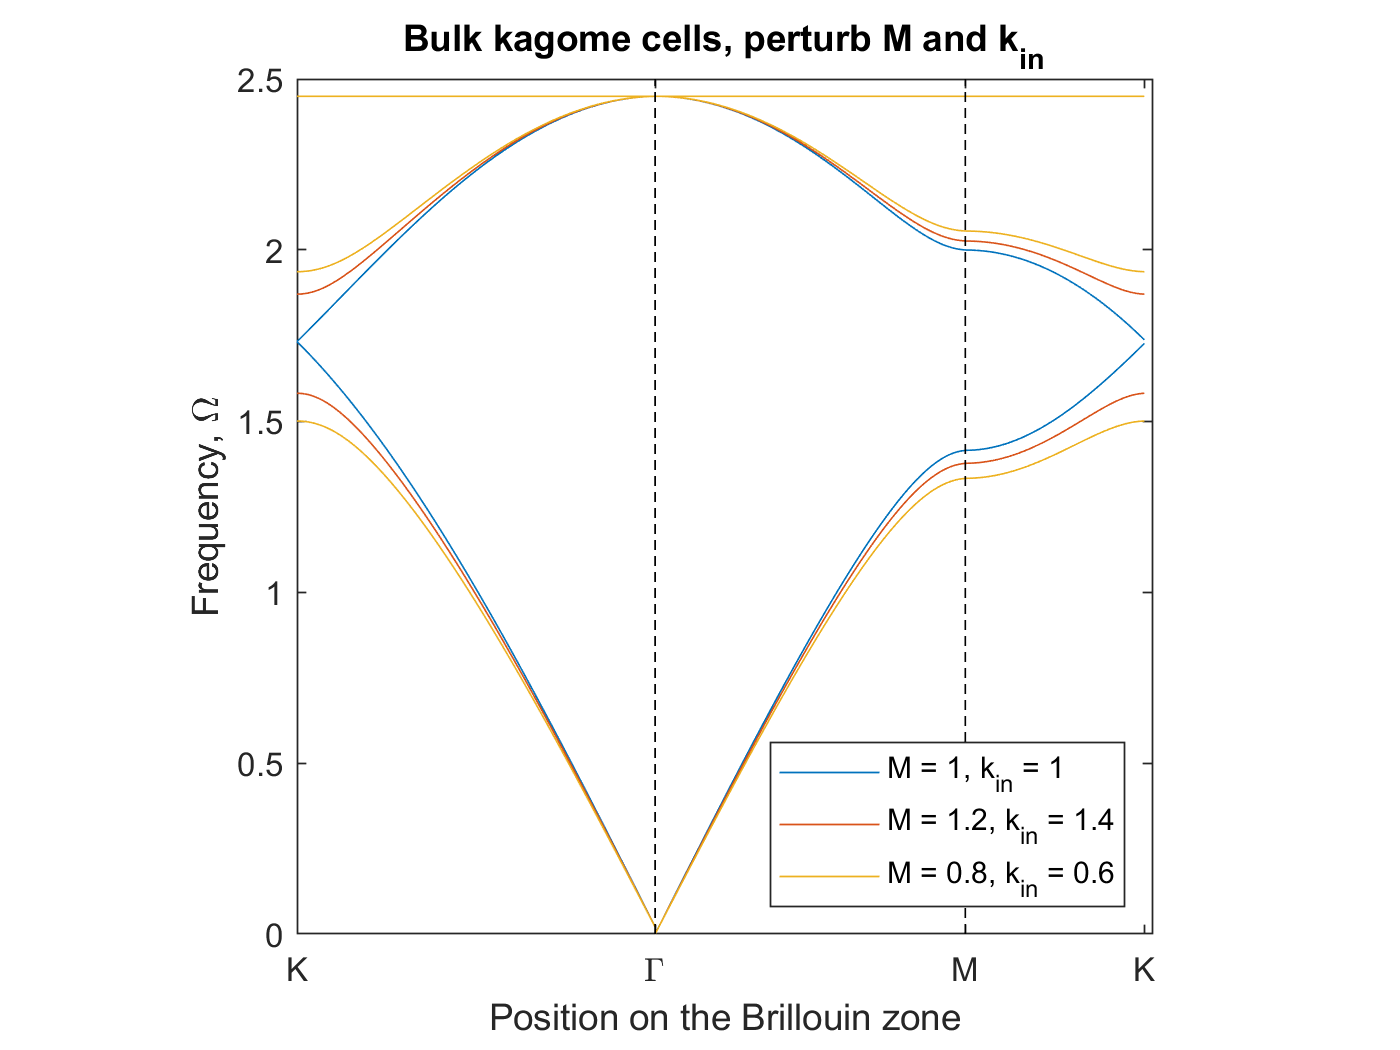
\includegraphics[width=0.8\textwidth]{imgs/kagomeperturb2.png}
\caption{\label{fig:kagome2} The effect of perturbing both the masses $M_i$ and
  the inner stiffness $k$ on the dispersion relation of the bulk kagome system,
  with all other parameters set to $1$.}
\end{figure}

\section{2d kagome strip}

\begin{figure}[!h]
\centering
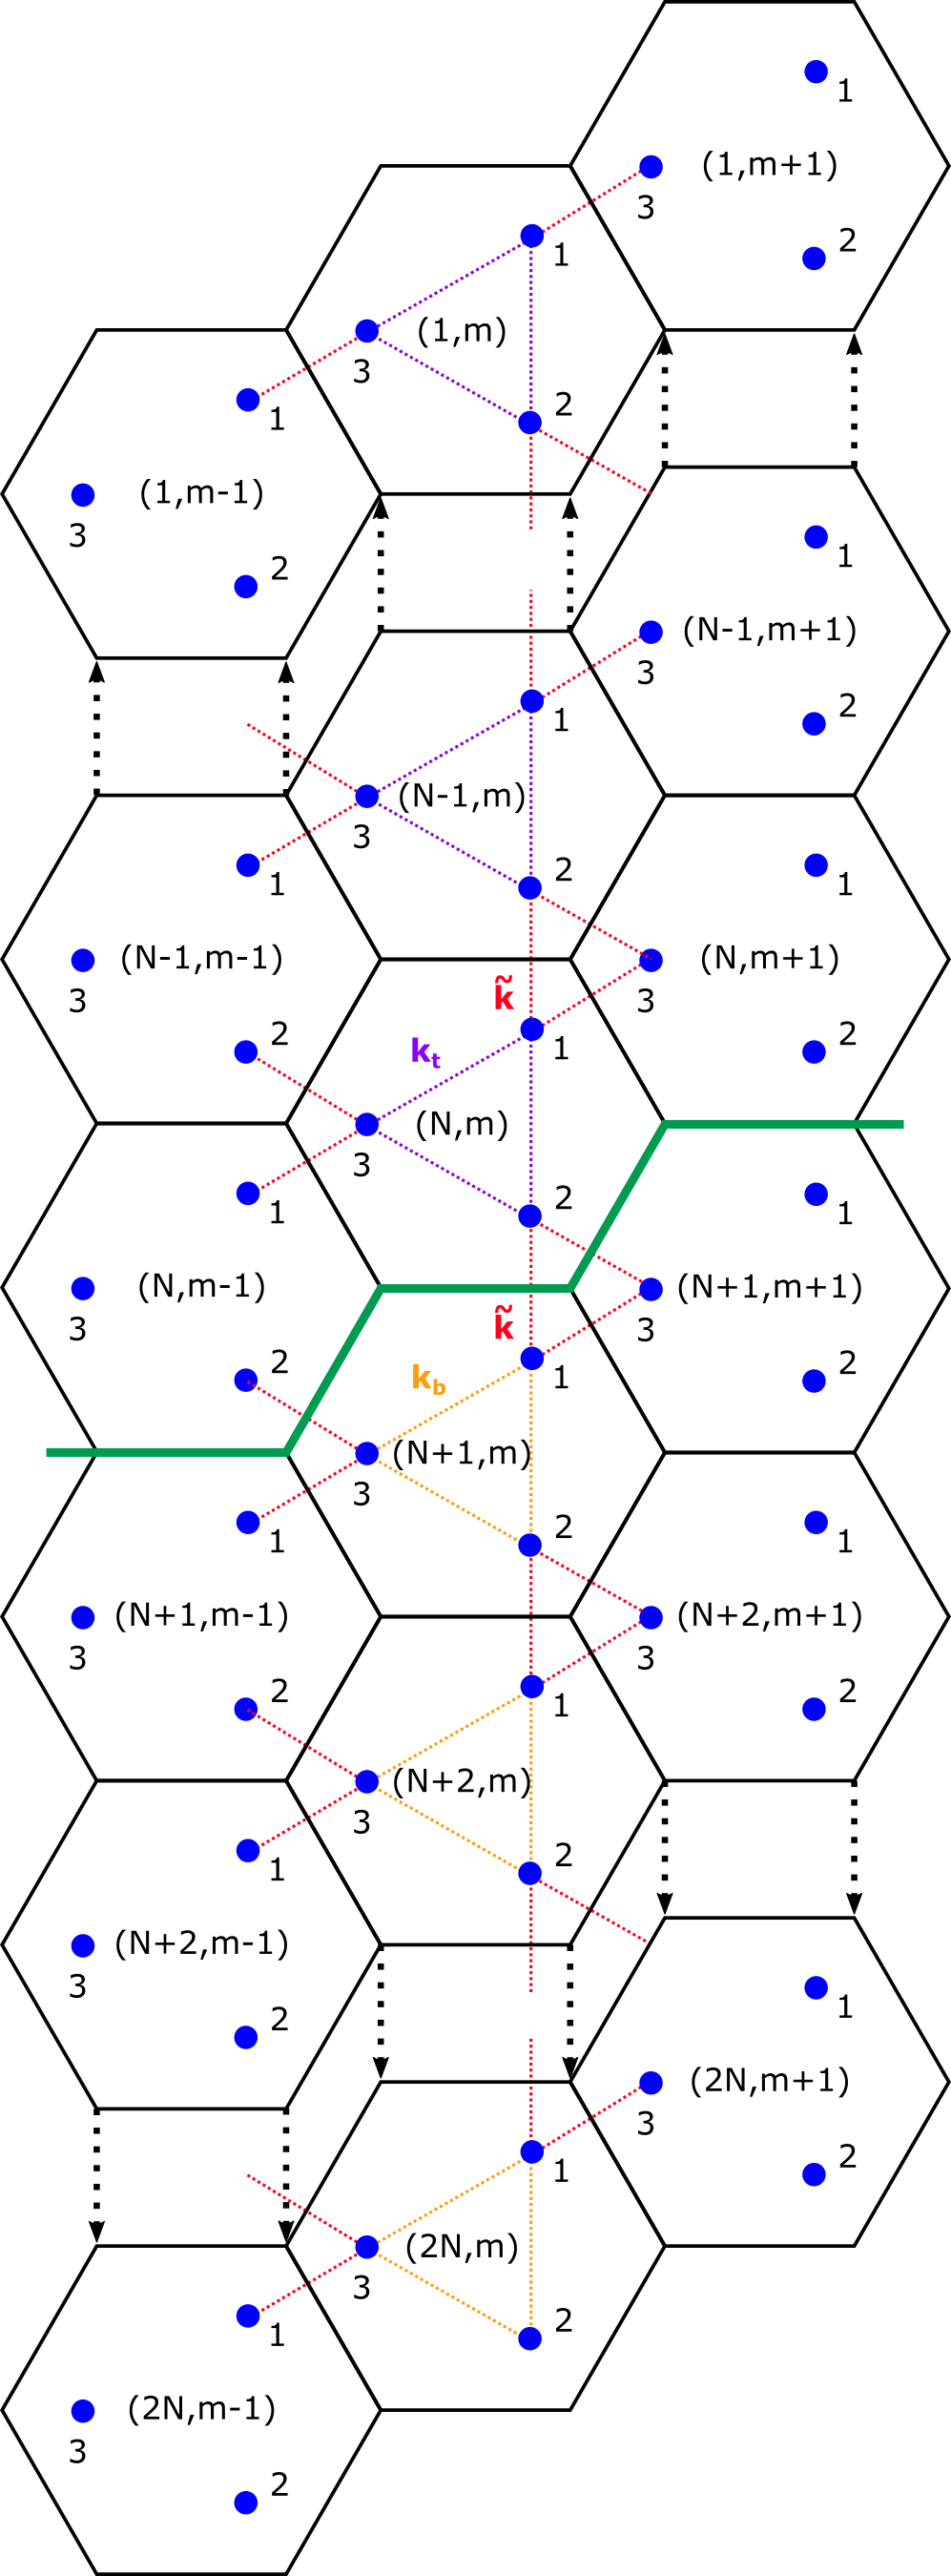
\includegraphics[width=0.4\textwidth]{imgs/kagomestripmodel.png}
\caption{\label{fig:kagomestripmodel} Schematic view of the 2d kagome
  semi-infinite lattice made from an infinite number of strips connected
  side-by-side. Each strip is composed of 2N cells, with the top half of cells
  above the boundary (green) possessing a set of properties and the bottom half
  possessing a separate set of properties.}
\end{figure}

As we have just done in the hexagonal case, we assemble $2N$ kagome cells
together into a strip and form a semi-infinite lattice with these strips
connected left-to-right as shown in Figure~\ref{fig:kagomestripmodel}.

Using the same conventions as the hexagonal strip case and similarly imposing
rigid boundary conditions at the top and bottom edge, we can form the
eigen-problem

%\begin{align}
%  \matr{A}_{1,3(2N-1)+2}&=\matr{A}_{3(2N-1)+2,1}=-\tilde{k} \\
%  \matr{A}_{3,3(2N-1)+2}&=-\tilde{k}e^{-i\Delta_1} \\
%  \matr{A}_{3(2N-1)+2,3}&=-\tilde{k}e^{i\Delta_1} 
%\end{align} 

\begin{align}
  \left[\matr{A}\left(\kappa_{x},\kappa_{y}\right)-\matr{\Omega}\matr{M}\right]\vec{y}=\vec{0}
\label{eq:kagomestripeig}
\end{align}

where $\matr{A}$ is a $(2N \times 6) \times (2N \times 6)$ matrix with
$\matr{A}$ as defined in \eqref{eq:kagomeeig} repeated along the diagonal and
with the additional coupling terms added,
$\matr{\Omega}=\diag\left(\left\{\Omega_i^2\right\}\right)$,
$\matr{M}_{t}=\diag\left(\left\{M_{i,t}\right\}\right)$,
$\matr{M}_{b}=\diag\left(\left\{M_{i,b}\right\}\right)$,
\begin{align}
\matr{M}=\left[
\begin{array}{cccccc}
\matr{M}_{t}\\
 & \ddots &  &  & 0\\
 &  & \matr{M}_{t}\\
 &  &  & \matr{M}_{b}\\
 & 0 &  &  & \ddots\\
 &  &  &  &  & \matr{M}_{b}
\end{array}\right],
\end{align}

\begin{align}
\vec{y}=\left[
\begin{array}{c}
y_1^{(1)}\\
y_2^{(1)}\\
y_3^{(1)}\\
\vdots\\
y_1^{(2N)}\\
y_2^{(2N)}\\
y_3^{(2N)}\\
\end{array}\right],
\end{align}

Solving this with $M_{i,t}=M_{i,b}=k_t=k_b=\tilde{k}=1$ over the same
$\kappa$-space as the hexagonal system, gives us the dispersion relation in
Figure~\ref{fig:kagomestripdisper}.

\begin{figure}[!h]
\centering
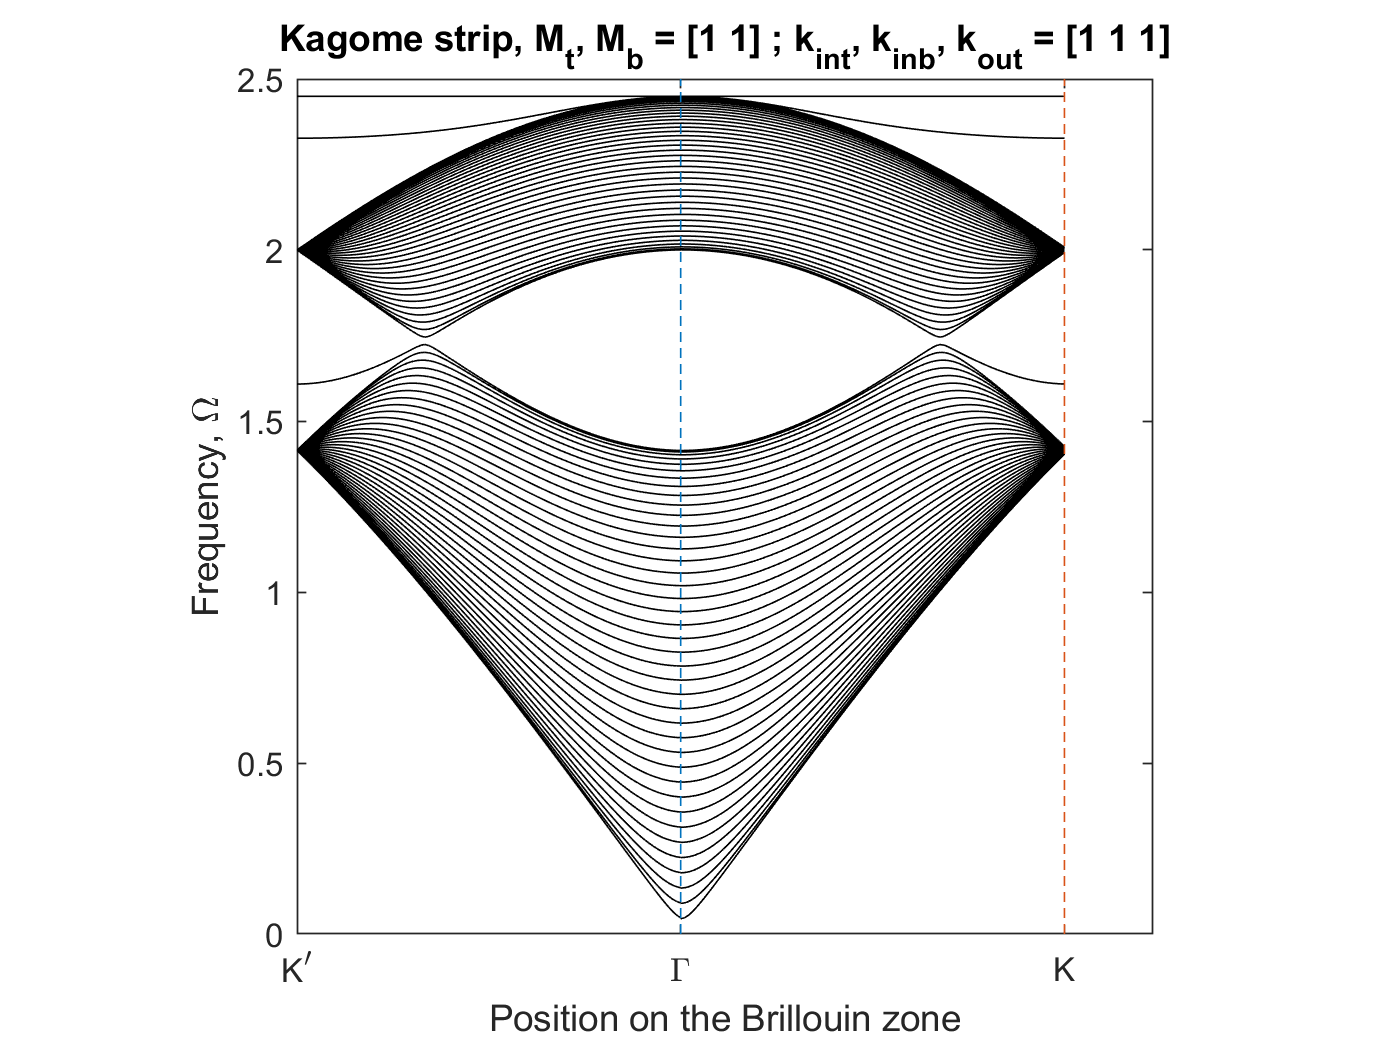
\includegraphics[width=0.8\textwidth]{imgs/kagomestrip.png}
\caption{\label{fig:kagomestripdisper} Dispersion relation of the semi-infinite
  kagome lattice with $2N=40$ (40 cells in total) with
  $M_{i,t}=M_{i,b}=k_t=k_b=\tilde{k}=1$.}
\end{figure}

Now let us try to get the dispersion relation for the semi-infinite kagome
lattice where the top material is made of the kagome cells with increased $M_i$
and $k$ and the bottom material is made of kagome cells decreased $M_i$ and
$k$, as we used in Figure~\ref{fig:kagome2}.

\begin{figure}[!h]
\centering
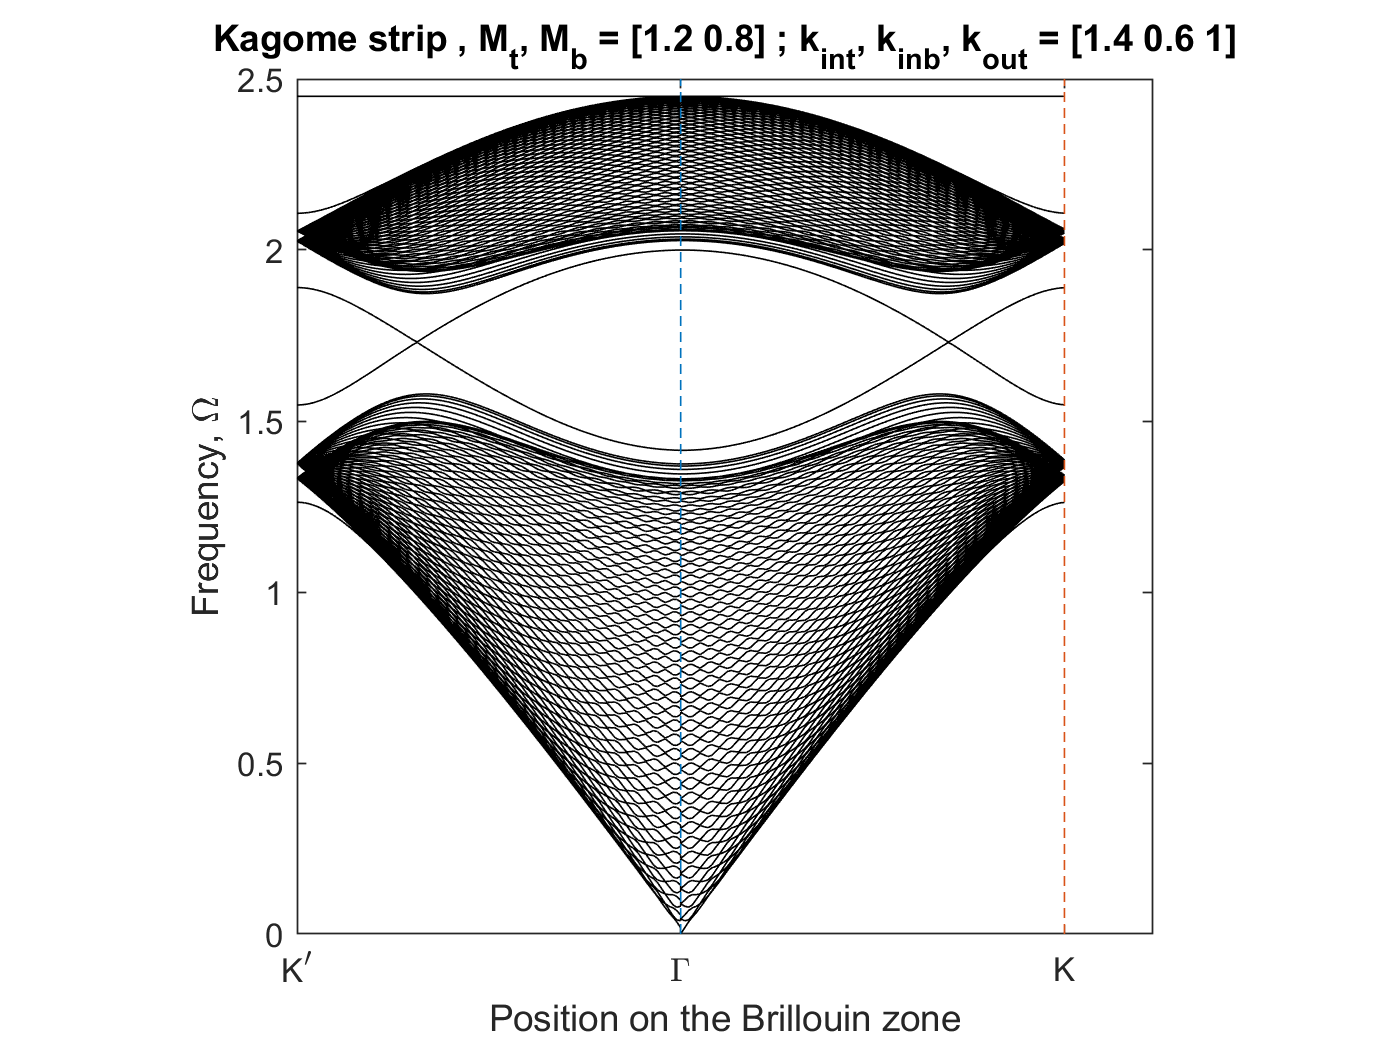
\includegraphics[width=0.8\textwidth]{imgs/kagomestripperturbed.png}
\caption{\label{fig:kagomeperturbed} Dispersion relation of the semi-infinite
  kagome lattice where the top material has a higher $M_i$ and $k$ than the
  bottom material, with all other parameters set to $1$.}
\end{figure}

Again, as in the hexagonal case, we have a bandgap with two well-defined
dispersion curves corresponding to edge states which live on the boundary.

Also, one thing interesting to note is that even with our perturbations, in
both the bulk and strip case we still have a flat band, as we have not broken
the symmetry of the cell as mentioned before!\cite{flatlines}

\chapter{Scattering simulation}
\label{scattering}
Finally after all our hard work of investigating the dispersion curves of
different lattices as well as finding out how to perturb them such that we form
a bandgap, we will actually simulate how a wave of a certain frequency
propagates and scatters through a finite portion of one of our lattices.

Similarly to how we joined cells together to from a strip, we will do the same
and join strips to form a finite lattice. We may then reframe our eigen-problem
systems in reciprocal space into linear systems in physical space. From there,
we can solve the linear systems to see how the energy or wave moves throughout
the entire space. All we need to do is pick a frequency for the wave we want to
simulate as well as where we want the source of excitation to be.

From the dispersion relations, we know which frequency waves are able to
propagate across the lattice and which frequencies are not transmitted through
the lattice. As we have discussed before in Chapter \ref{formstrip}, we know
that there are certain frequencies which are only able to propagate along the
interface of the strips and not anywhere else in the lattice. These are the
frequencies which we will be simulating.
%TODO: Different shape of lattices to bend waves?

\section{Our linear system in physical space}
Before we can run our scattering simulations, which essentially is solving for
the displacements of masses in our finite lattice, we need to form the system
to solve. This actually turns out to be really similar to the eigen-problems we
had earlier (albeit with a much larger matrix involved!). It is also useful to
note that the following derivation works just as well for systems of any shape
as long as we have formed the eigen-problem as before, as we will reuse the
variables in the eigen-problem here.
 
The key idea in this is that we can pick and choose the frequency, $\Omega$,
and so by just
%TODO: Finish derivation of linear system

With this linear system set up, let us take a look at the physical spaces in
which we will run these simulations.

\section{2d hexagonal finite lattice}
\begin{figure}[!h]
\centering
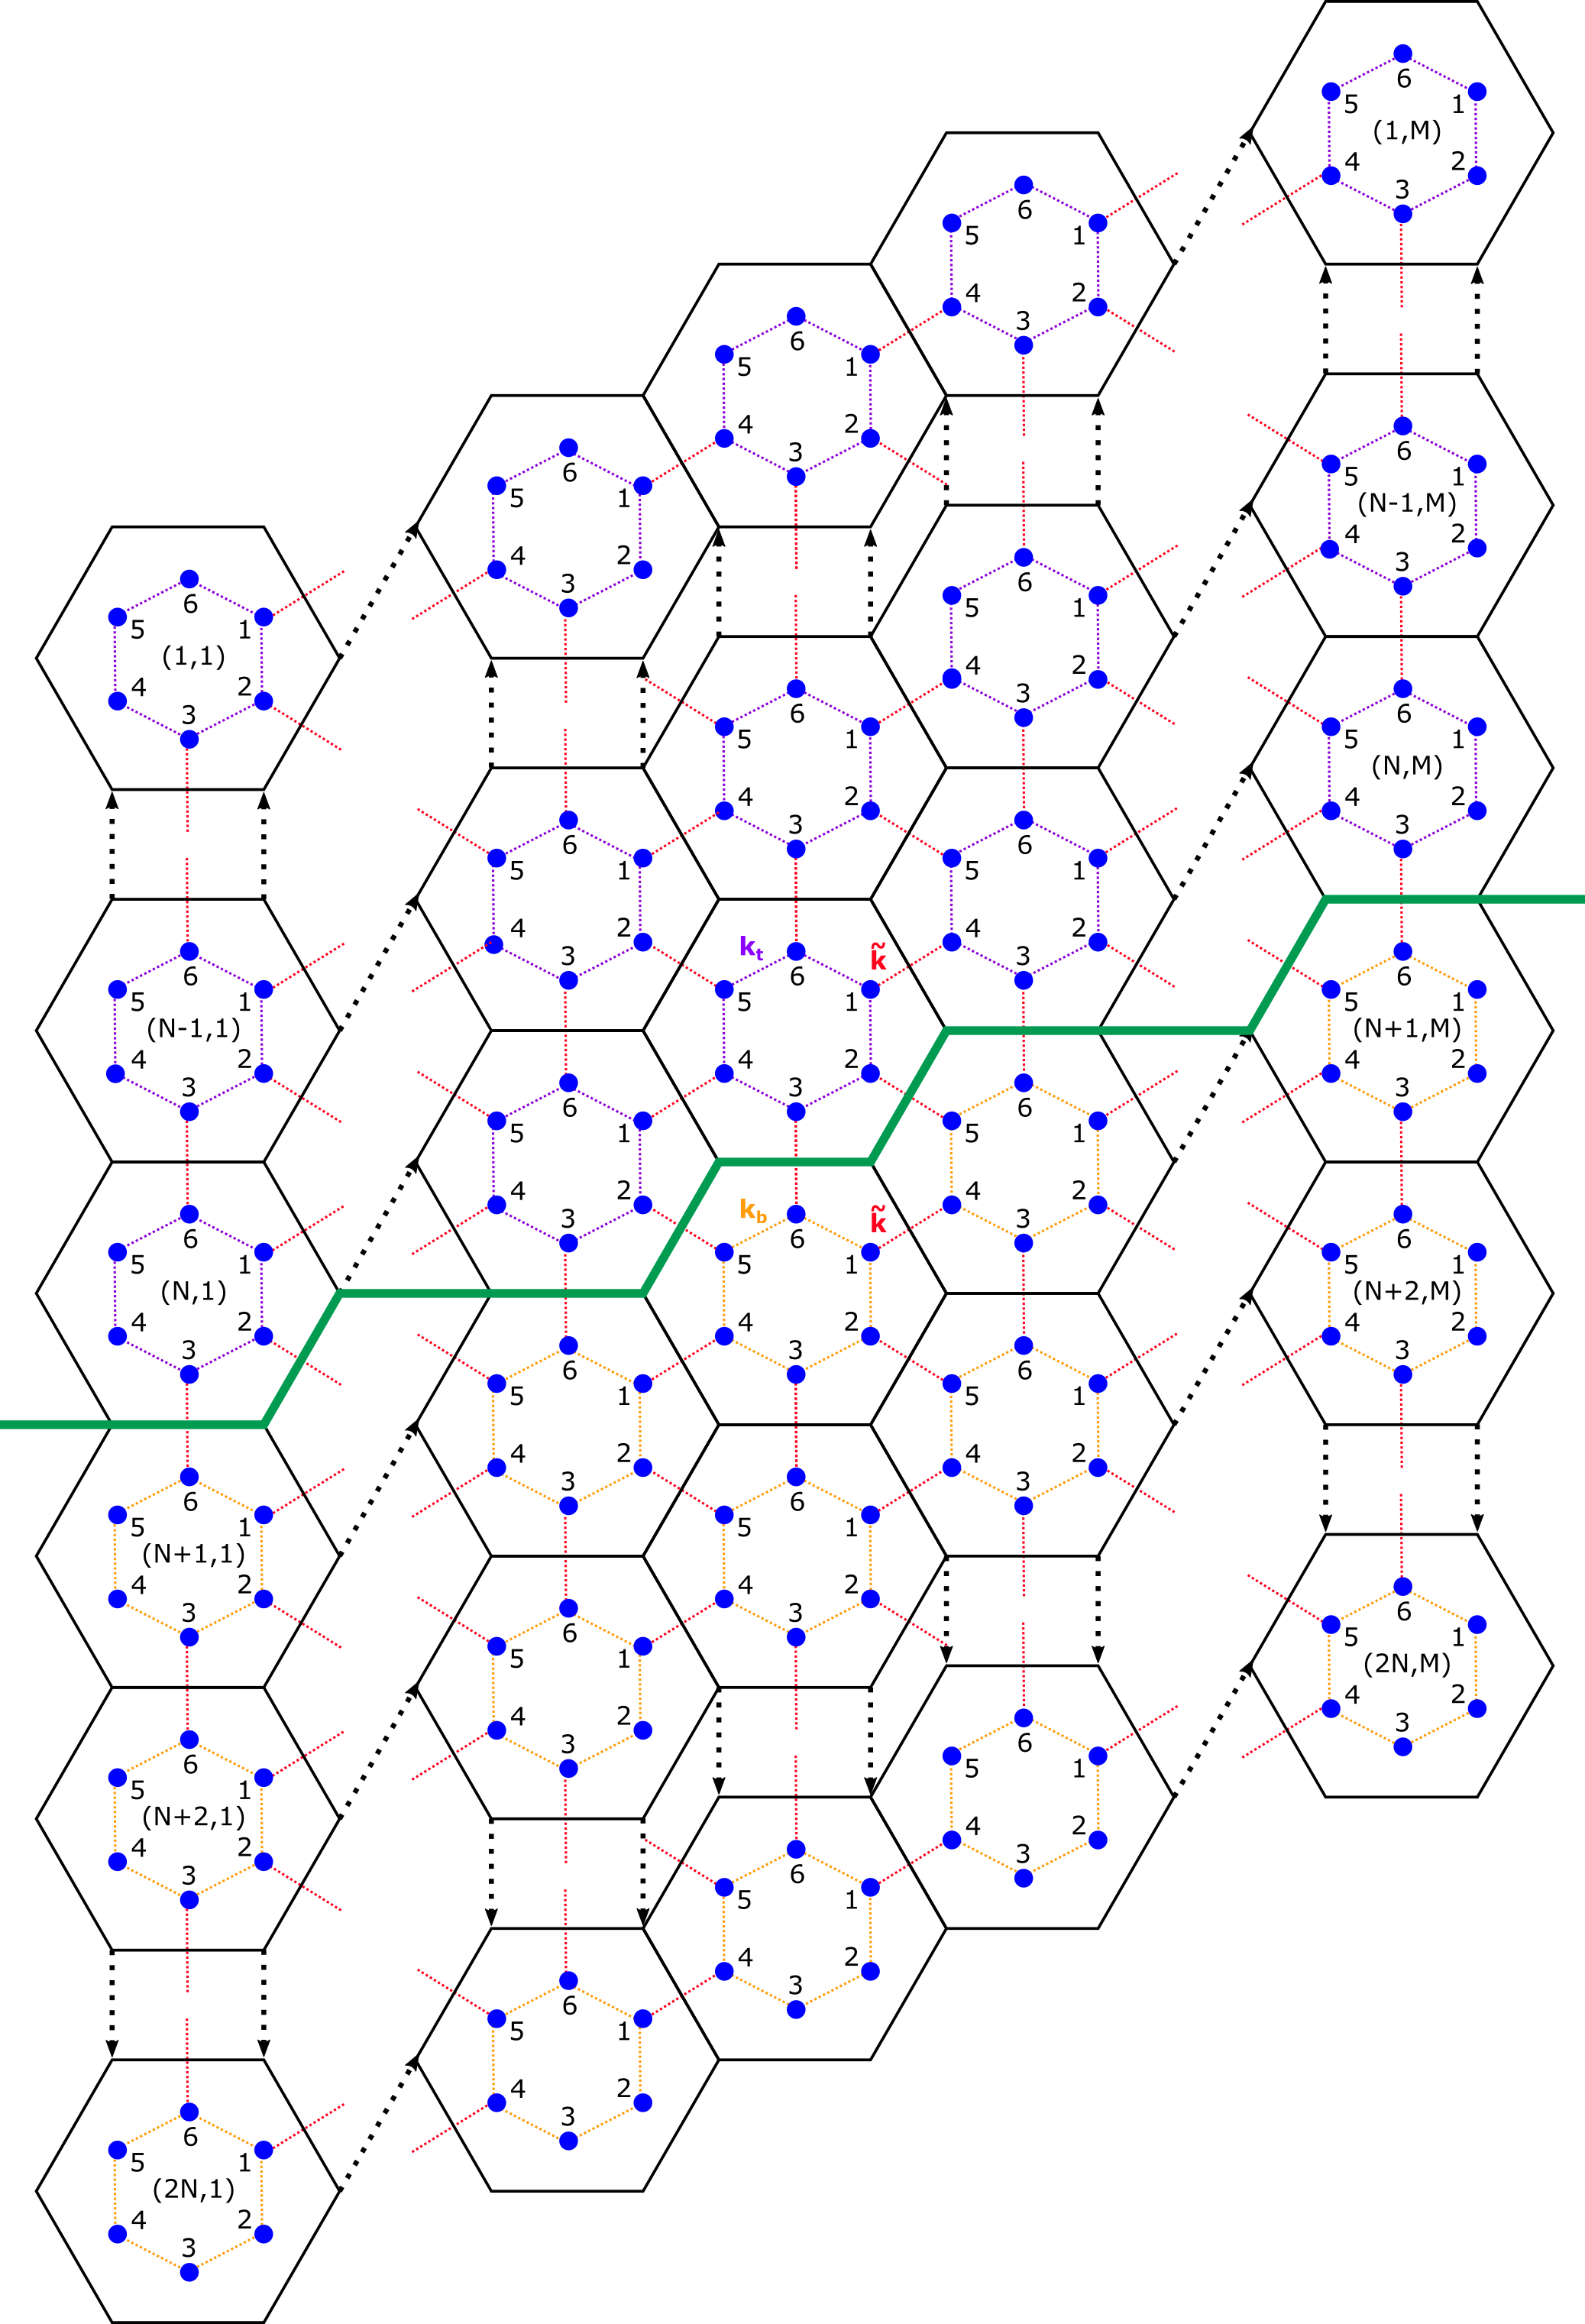
\includegraphics[width=0.8\textwidth]{imgs/hexfinitemodel.png}
\caption{\label{fig:hexfinscheme} Schematic view of the finite hexagonal
  lattice formed from the joining of strips side-by-side, where the strips
  themselves are formed from two different halves as in Chapter
  \ref{perturbed}.  Note the conditions imposed at the boundaries (masses at
  boundaries have no connections outside the lattice).}
\end{figure}

Specifically, we will be running our following simulations on the arrangement
of cells in Figure~\ref{fig:hexstdfinlattice}.

\begin{figure}
  \centering
  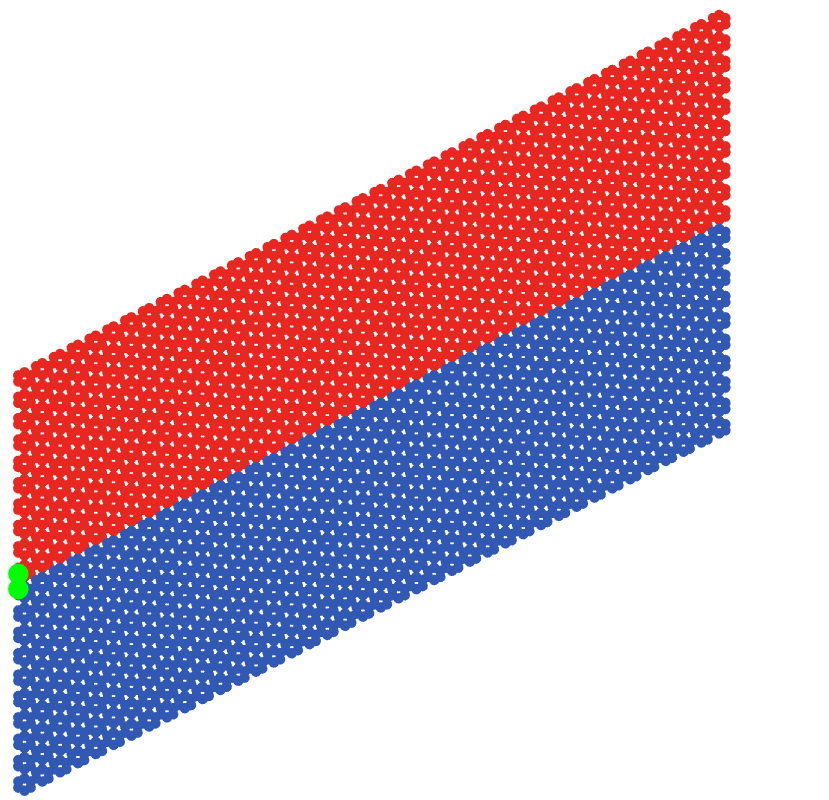
\includegraphics[width=0.6\linewidth]{imgs/hexstdfinlattice.png}
  \caption{Arrangement of hexagonal cells ($2N=20$, $M=40$), with red and blue
    being different materials, and source of excitation at the green masses.}
  \label{fig:hexstdfinlattice}
\end{figure}

\subsection{Alternating masses}

In this section we will run scattering simulations on the physical lattice as
described in Chapter \ref{perturbaltmass} with the alternating masses.

Now, we can run our simulations for another frequency we want, but we know from
our dispersion relations that most frequencies (those outside the special
dispersion curves corresponding to the edge states) will just propagate
throughout the lattice and so we would not get any discernible patterns of
movement. An example can be found in Figure~\ref{fig:randscat}.

\begin{figure}
\centering
\begin{subfigure}[b]{.5\textwidth}
  \centering
  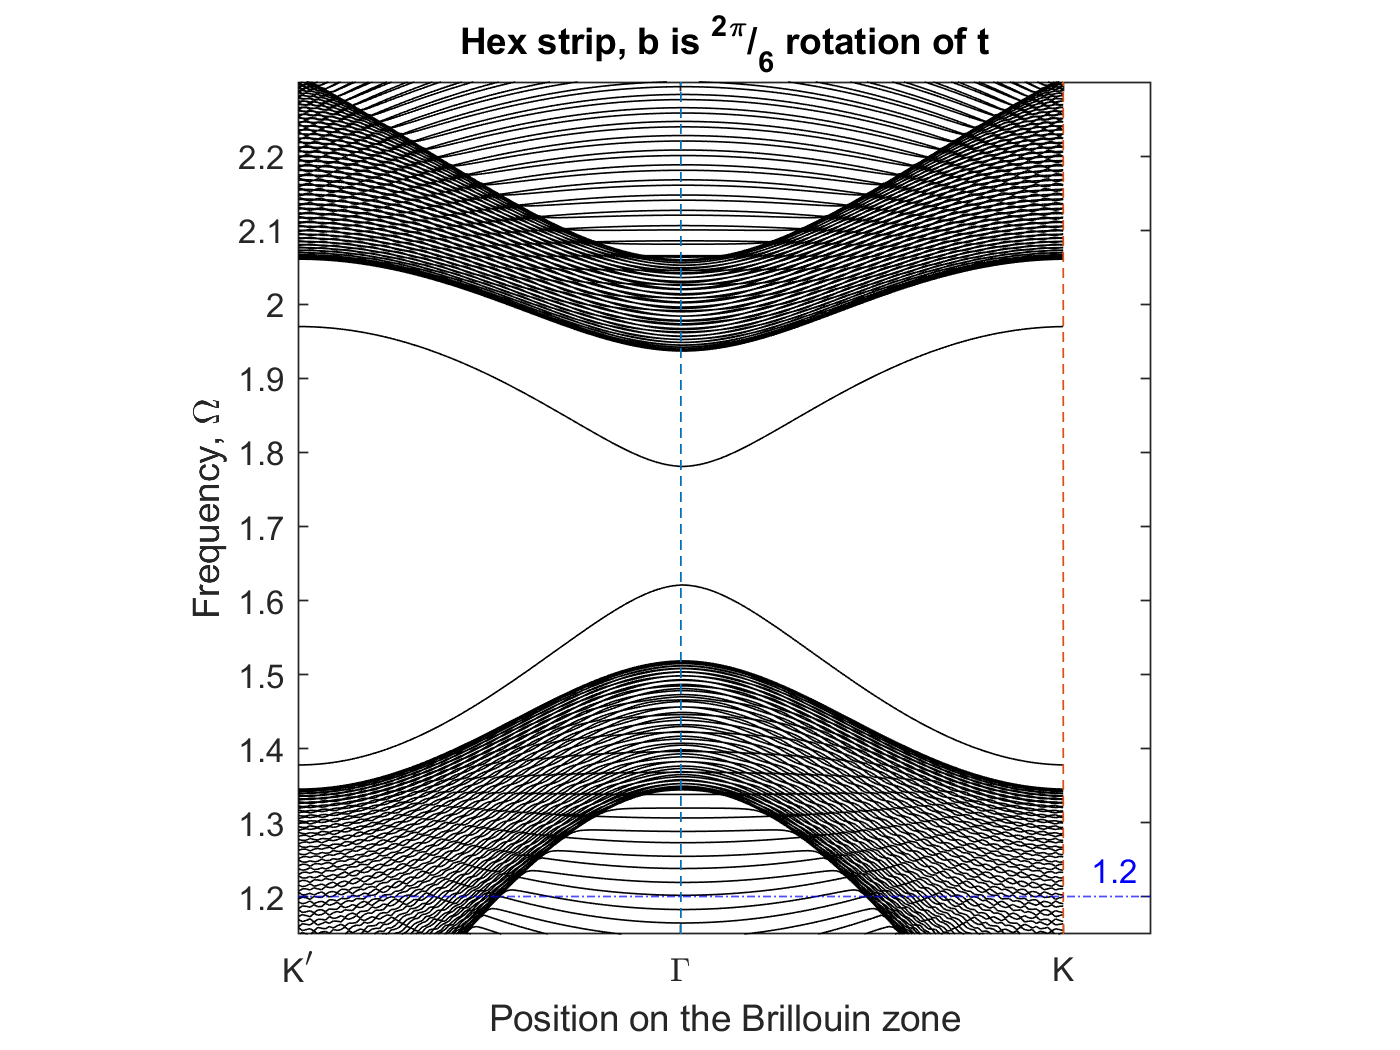
\includegraphics[width=1.1\linewidth]{imgs/hexstripperturbMrotatedrand.png}
  \caption{Zoomed in look of Figure~\ref{fig:hexstripMrotated} near the bandgap.}
\label{fig:sub1}
\end{subfigure}%
\begin{subfigure}[b]{.5\textwidth}
  \centering
  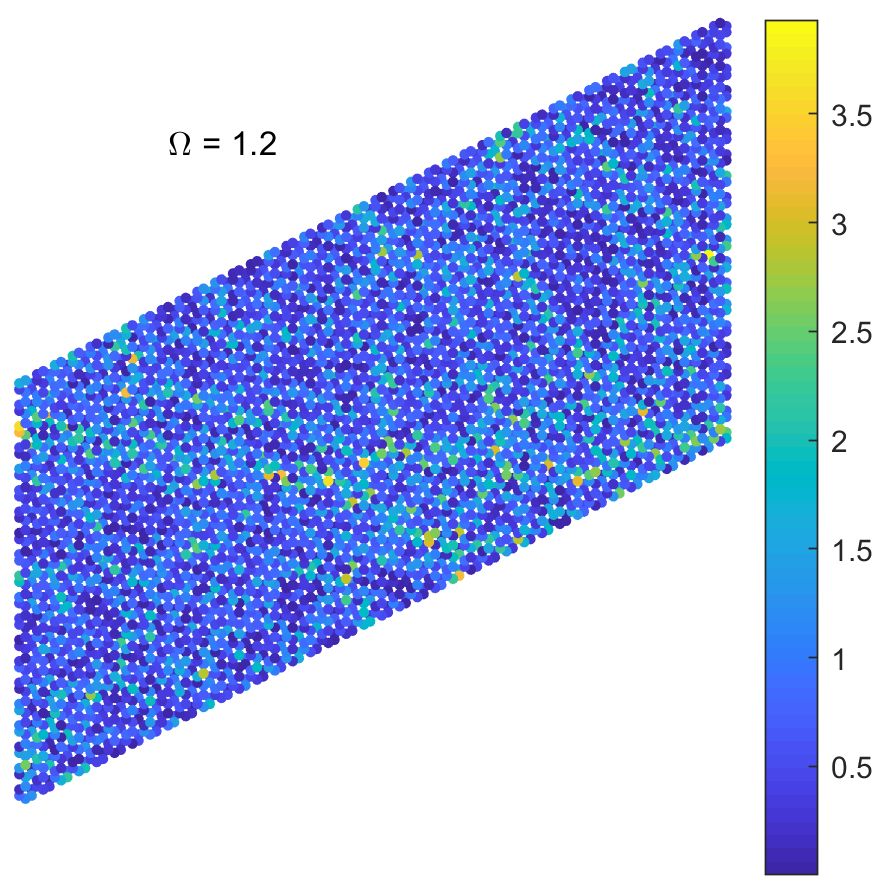
\includegraphics[width=1\linewidth]{imgs/hexstdrandscat.png}
  \caption{The plot of $|y_i|$ for each mass in each cell.}
  \label{fig:sub2}
\end{subfigure}
\caption{Simulation of scattering on the hexagonal finite lattice in
  Figure~\ref{fig:hexstdfinlattice} with the alternating masses as defined in
  Figure~\ref{fig:hexstripMrotated} with $\Omega = 1.2$.}
\label{fig:randscat}
\end{figure}

As we are interested in being able to direct waves to our liking, it is much
more exciting to fire a frequency which is only able to travel along the
boundary. So let use the same system as in Figure~\ref{fig:randscat} again, but
using $\Omega = 1.6$ instead as we can see in
Figure~\ref{fig:hexstripMrotatedzooms1} that the dispersion curve for that edge
mode lives in the bandgap.

\begin{figure}
\centering
\begin{subfigure}[b]{.5\textwidth}
  \centering
  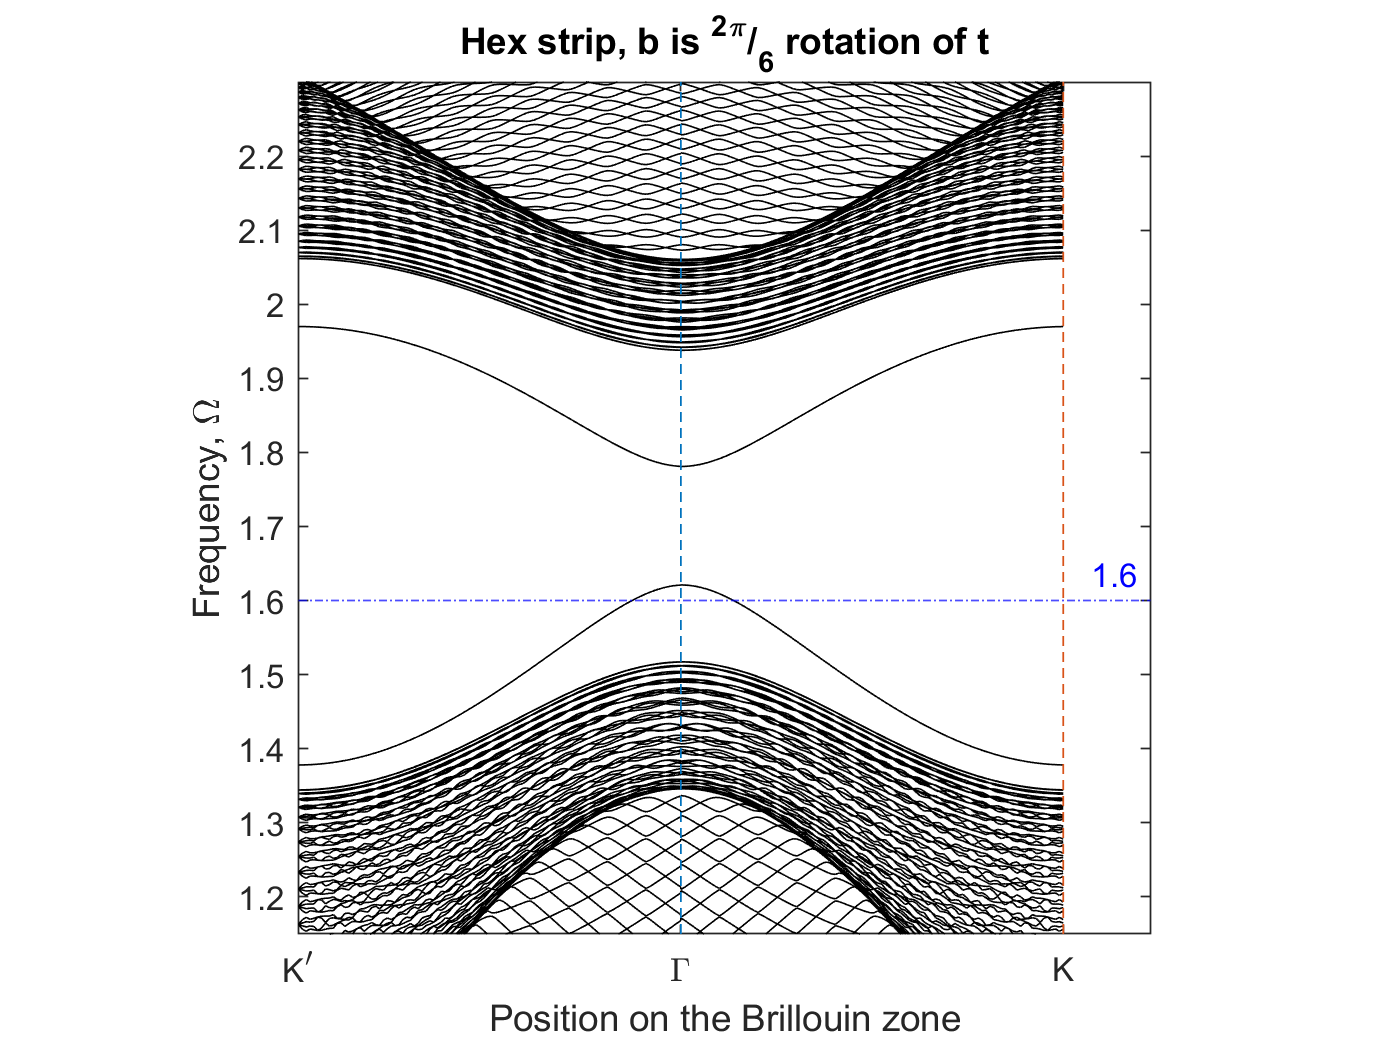
\includegraphics[width=1.1\linewidth]{imgs/hexstripperturbMrotatedzoom.png}
  \caption{Zoomed in look of Figure~\ref{fig:hexstripMrotated} near the bandgap.}
  \label{fig:hexstripMrotatedzooms1}
\end{subfigure}%
\begin{subfigure}[b]{.5\textwidth}
  \centering
  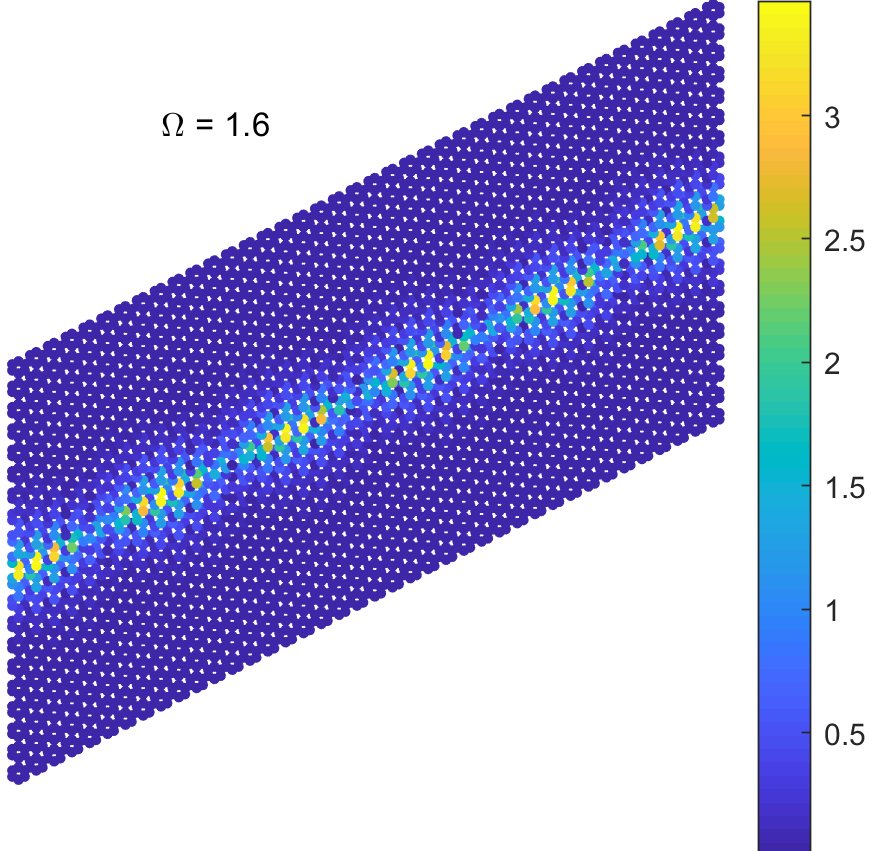
\includegraphics[width=1\linewidth]{imgs/hexstdrotstraight.png}
  \caption{The plot of $|y_i|$ for each mass in each cell.}
  \label{fig:sub2}
\end{subfigure}
\caption{Simulation of scattering on the hexagonal finite lattice in
  Figure~\ref{fig:hexstdfinlattice} with the alternating masses as defined in
  Figure~\ref{fig:hexstripMrotated} with $\Omega = 1.6$.}
\label{fig:hexstdrotstraight}
\end{figure}

Wonderful! Finally after all our hard work we can see in
Figure~\ref{fig:hexstdrotstraight} that the wave or energy forced into the
system is only propagating along the straight line. This effectively means that
we can control the direction of propagation of waves through our lattice and
not have it diffuse or \textit{leak} out into the other parts of the lattice.
Of course our next thought would be to see if it is possible to send the energy
around bends and more complex boundaries, which is what we discuss in Chapter
\ref{complexbends}.

\subsection{Varying mass and stiffnesses}
In this section we will take a look at running scattering simulations as above
but for the physical system discussed in Chapter \ref{perturbMk}.

\begin{figure}
\centering
\begin{subfigure}[b]{.5\textwidth}
  \centering
  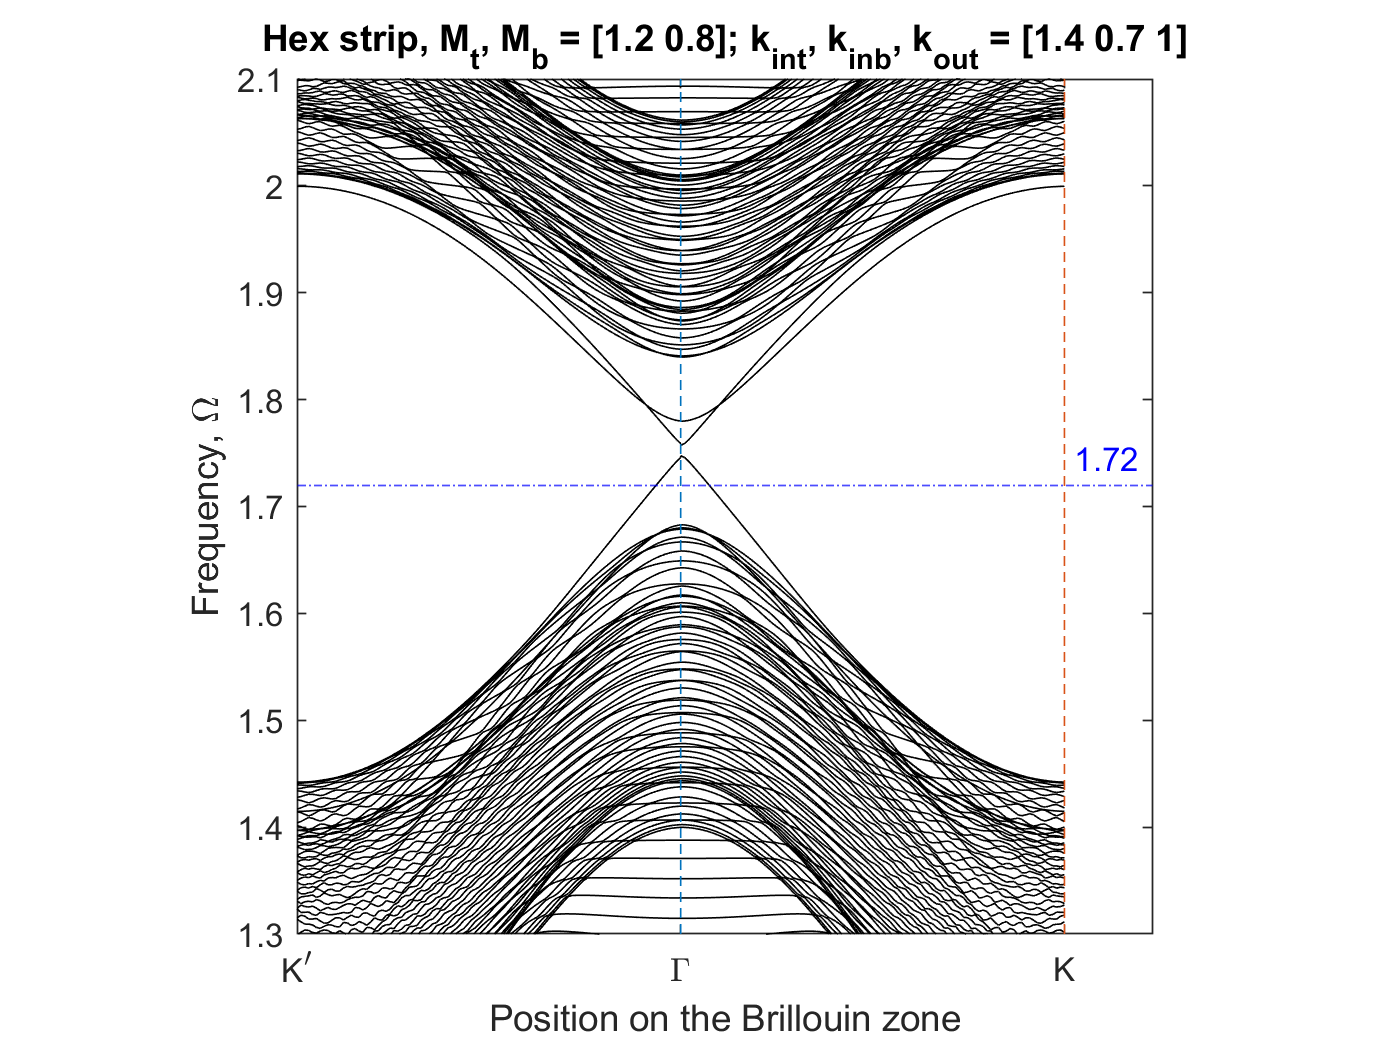
\includegraphics[width=1.1\linewidth]{imgs/hexstripperturb2zoom.png}
  \caption{Zoomed in look of Figure~\ref{fig:hexstrip2} near the bandgap.}
  \label{fig:sub1}
\end{subfigure}%
\begin{subfigure}[b]{.5\textwidth}
  \centering
  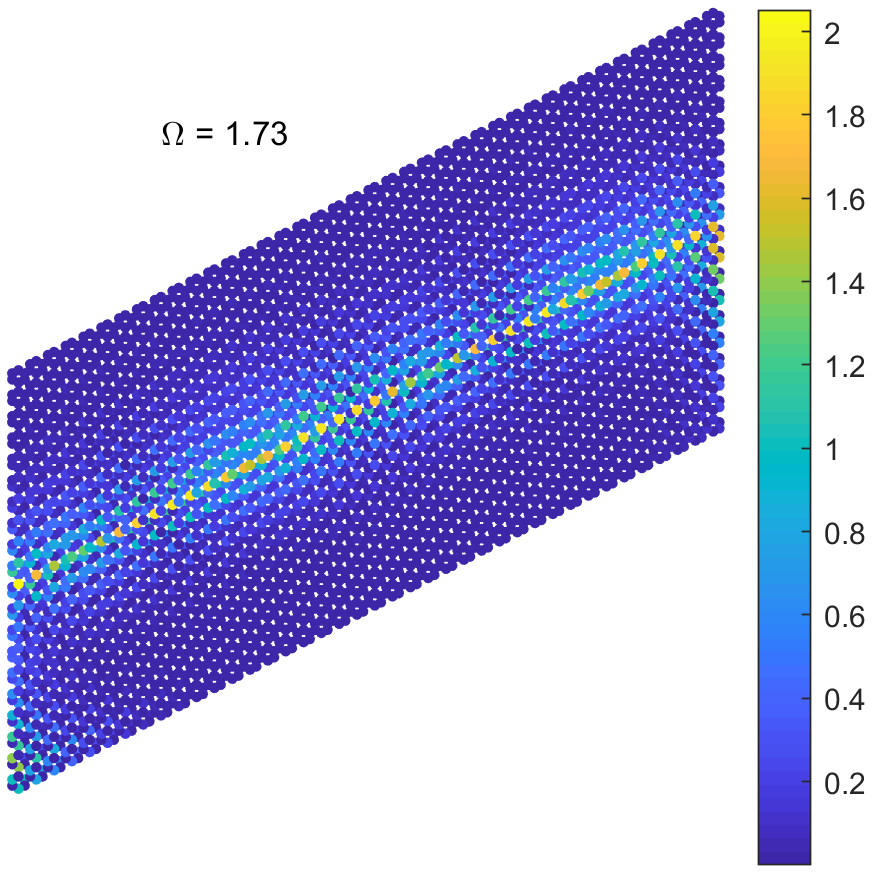
\includegraphics[width=1\linewidth]{imgs/hexstdMk.png}
  \caption{The plot of $|y_i|$ for each mass in each cell.}
  \label{fig:sub2}
\end{subfigure}
\caption{Simulation of scattering on the hexagonal finite lattice in
  Figure~\ref{fig:hexstdfinlattice} with the top having a greater $M$ and $k$
  than the bottom as defined in Figure~\ref{fig:hexstrip2} with $\Omega =
  1.72$.}
\label{fig:hexstdMk}
\end{figure}

\section{2d kagome finite lattice}
\begin{figure}[!h]
\centering
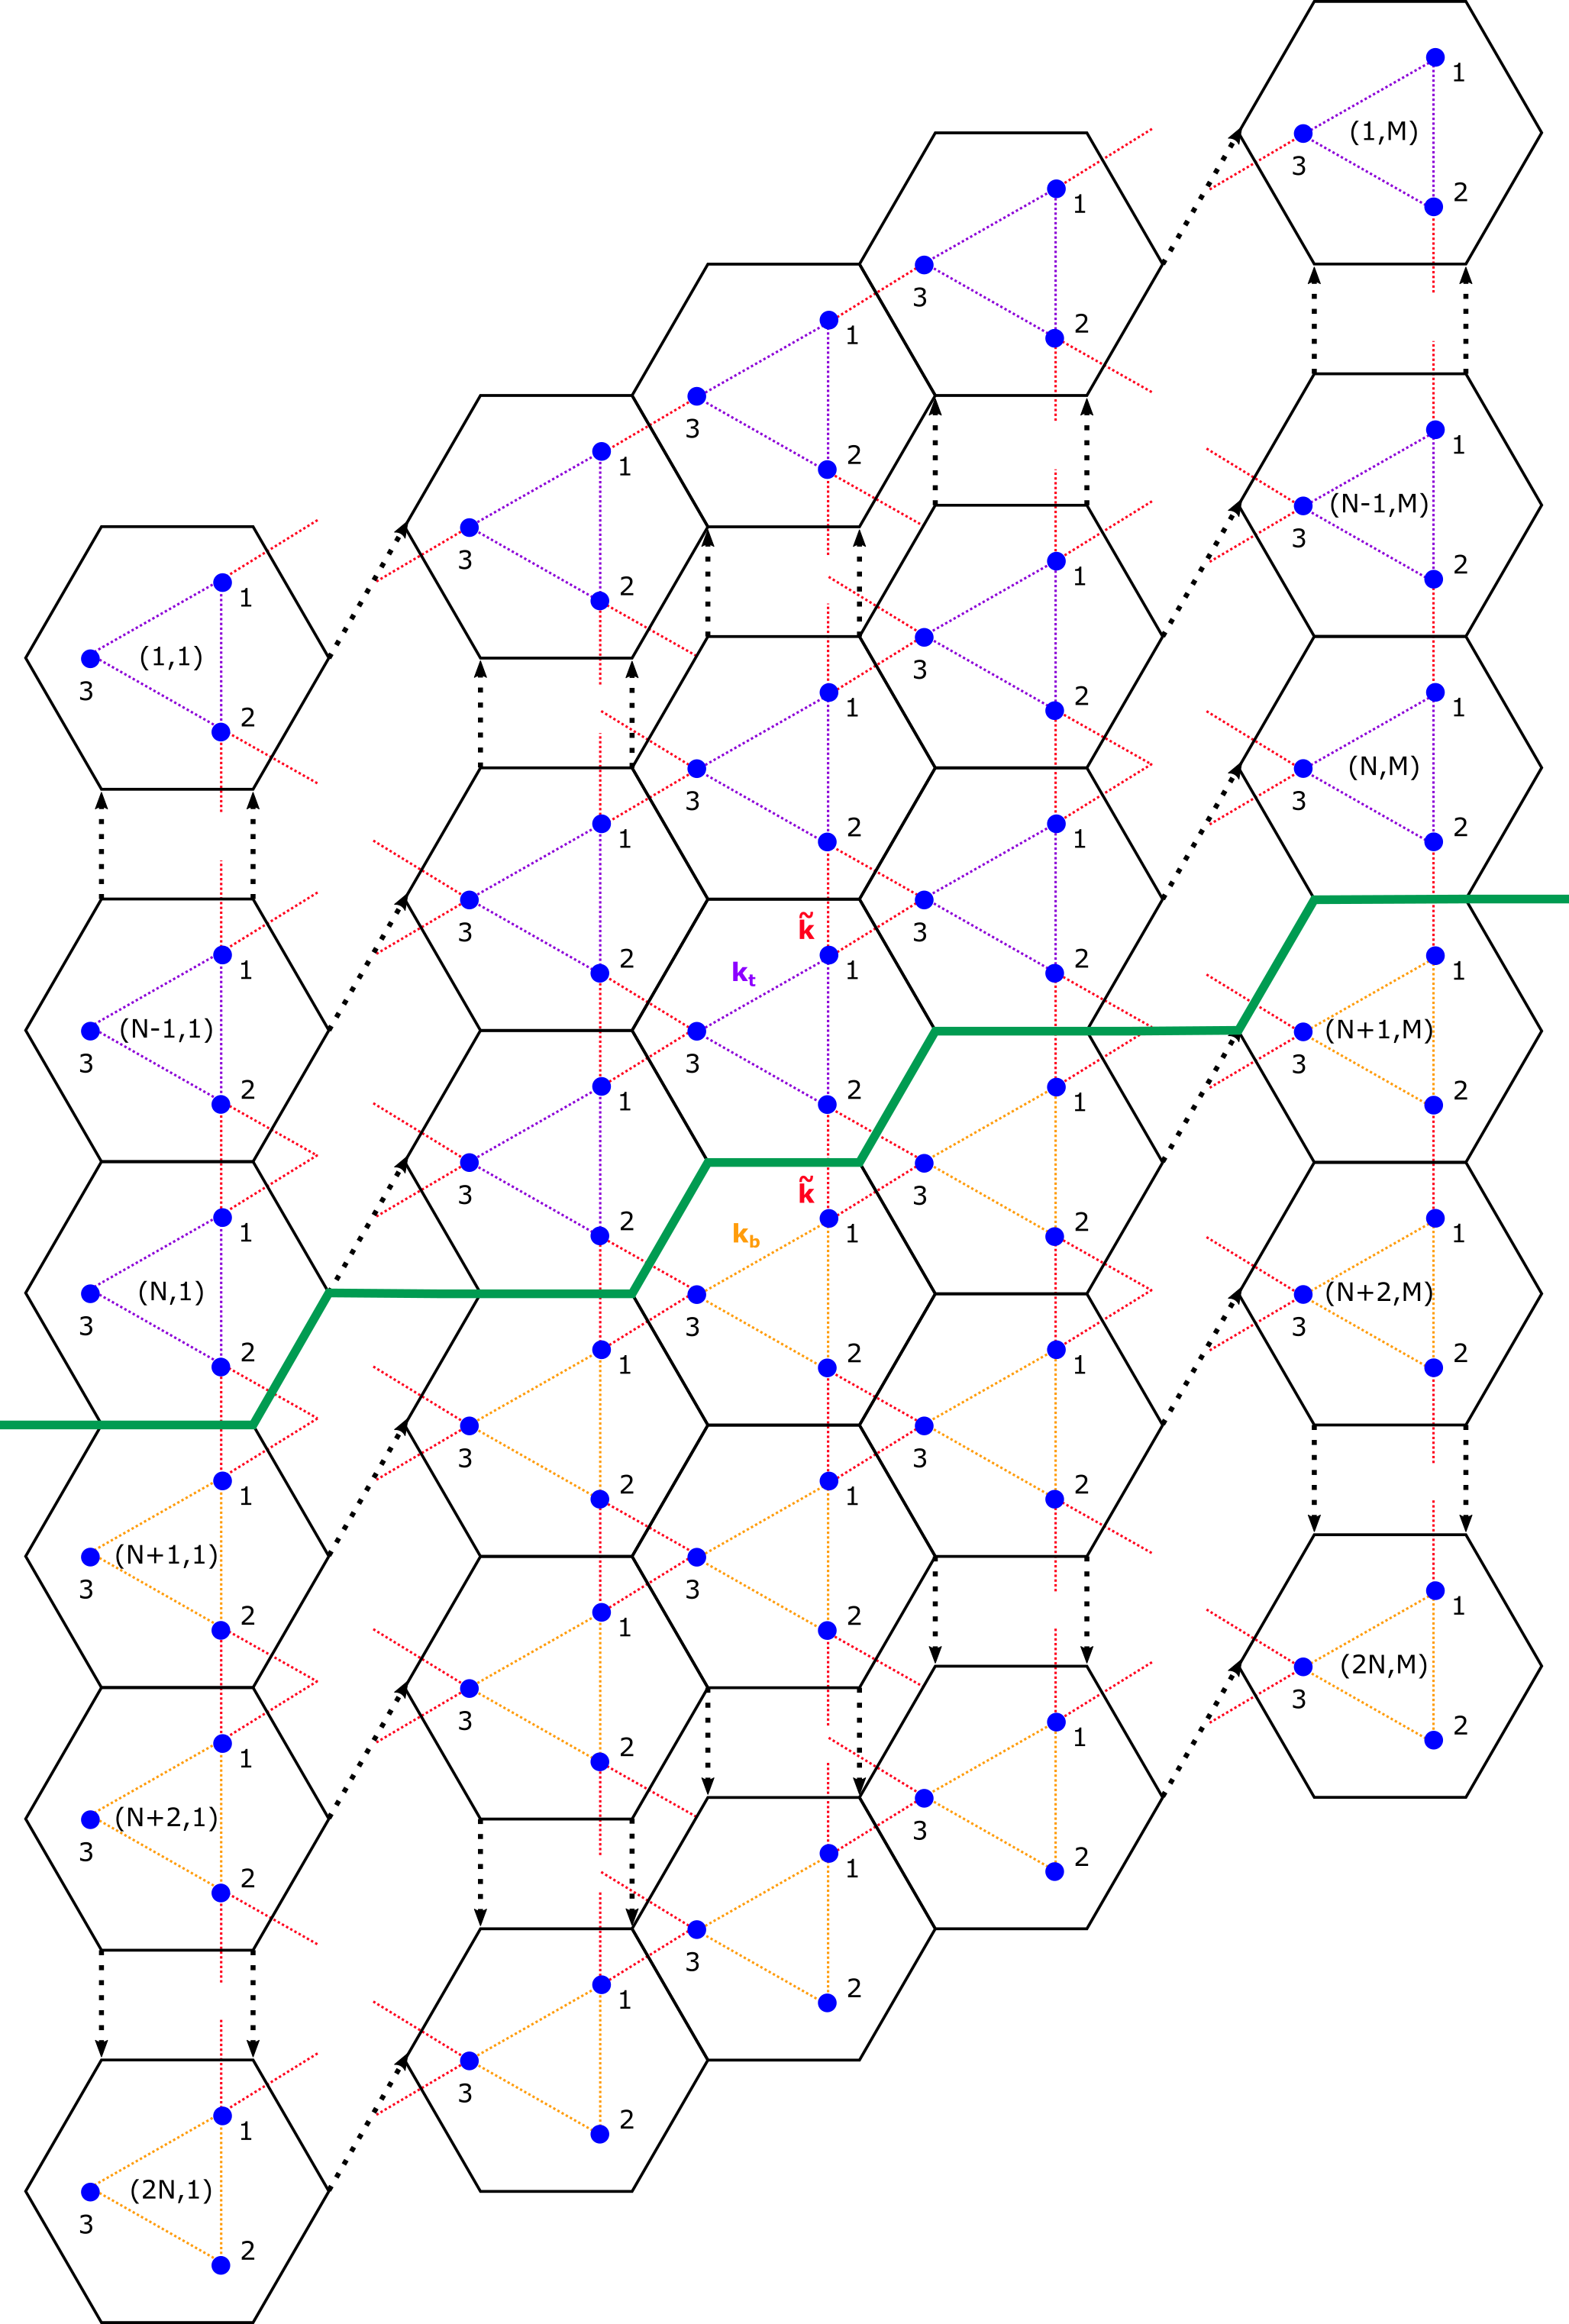
\includegraphics[width=0.8\textwidth]{imgs/kagomefinitemodel.png}
\caption{\label{fig:kagomefinscheme} Schematic view of the finite kagome
  lattice formed from the joining of strips side-by-side, where the strips
  themselves are formed from two different halves as in Chapter
  \ref{perturbed}. Note the conditions imposed at the boundaries (masses at
  boundaries have no connections outside the lattice).}
\end{figure}

\section{Complex bends}
\label{complexbends}
Now that we have built up the foundation of how we can force a wave to
propagate in a specific direction in a topologically repeating material or
metamaterial, we want to see just how robust this phenomenon is based on the
shape of the boundary, i.e. just how much can we bend the wave?

\textit{Note:}Since we have already shown that this can be done for both the
hexagonal and kagome lattice, in this section we will only be running our
simulations for the hexagonal lattice to avoid duplication, as we are just
exploring whether the shape of the boundary affects the scattering.
Furthermore, we will specifically be using the same top and bottom cels as
Figure~\ref{hexstdrotstraight}, which is with alternating masses as defined in
Figure~\ref{fig:hexstripMrotated}.

\subsection{Gentle and sharp straight bends}
So far we have seen just straight line boundaries, but can this work for bent
boundaries too? Due to the way we set up our lattice (with the strips getting
higher as we go from left to right), there are two kinds of bends we can make
straight away. The 'gentle' bend where we bend the boundary upwards, and the
'sharp' bend where we bend the boundary downwards.

\begin{figure}
\centering
\begin{subfigure}[b]{.5\textwidth}
  \centering
  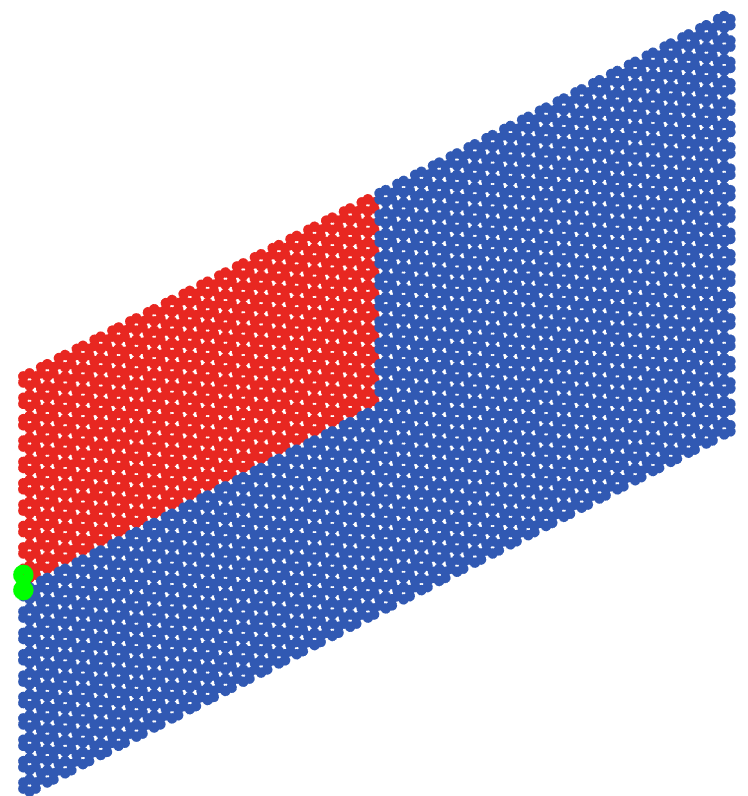
\includegraphics[width=0.8\linewidth]{imgs/gentlebendarr.png}
  \caption{Arrangement of cells to form a gentle bend.}
  \label{fig:sub1}
\end{subfigure}%
\begin{subfigure}[b]{.5\textwidth}
  \centering
  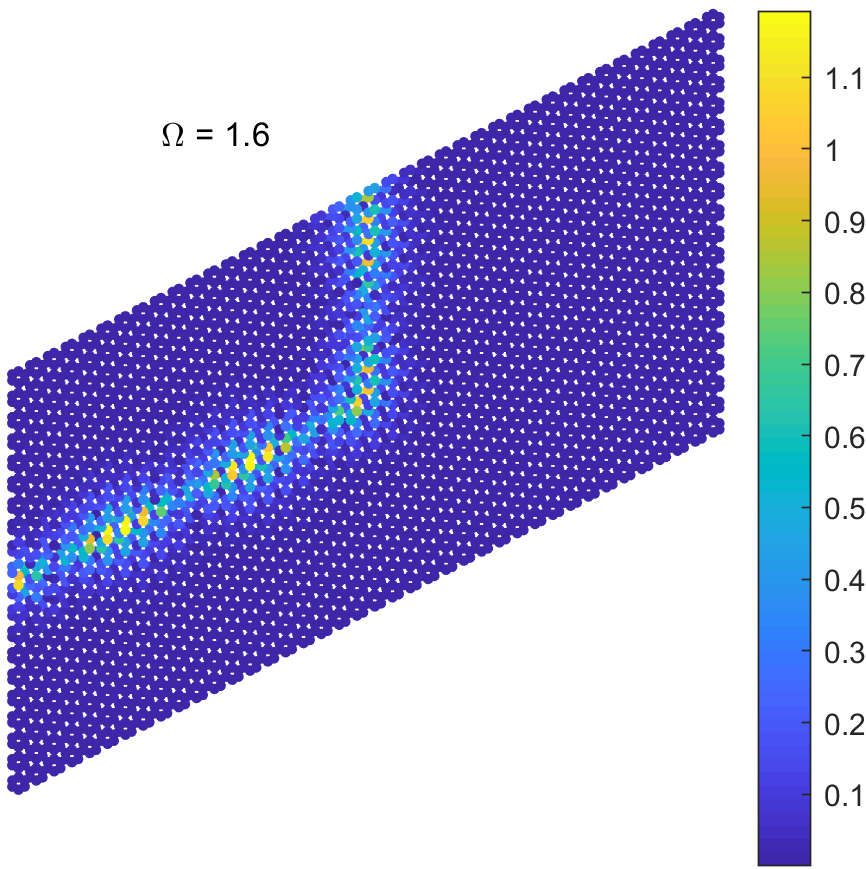
\includegraphics[width=1\linewidth]{imgs/gentlebendscat.png}
  \caption{The plot of $|y_i|$ for each mass in each cell.}
  \label{fig:sub2}
\end{subfigure}
\caption{Simulation of scattering on the hexagonal finite lattice with gentle
  bend.}
\label{fig:gentlebend}
\end{figure}

\begin{figure}
\centering
\begin{subfigure}[b]{.5\textwidth}
  \centering
  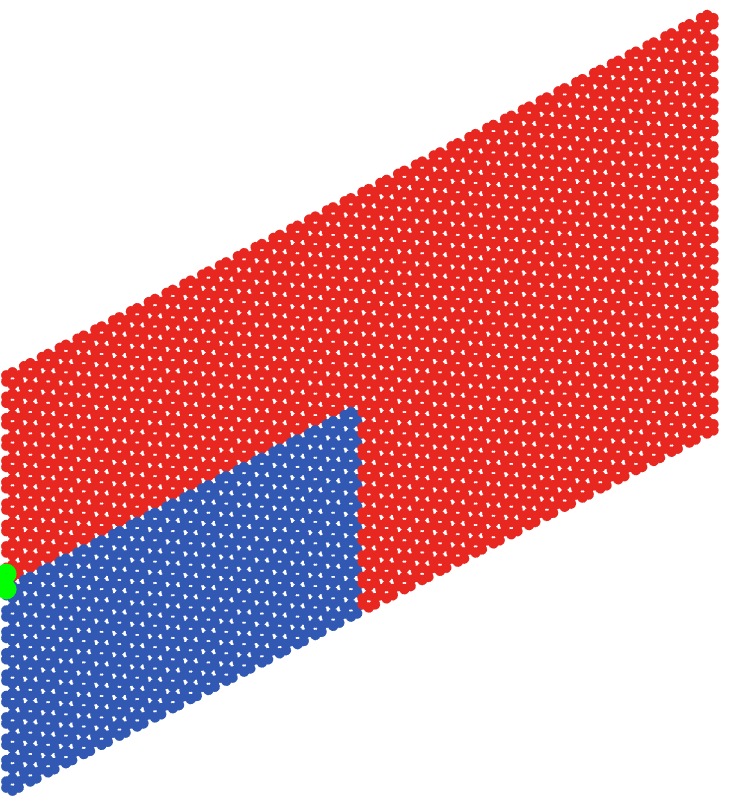
\includegraphics[width=0.8\linewidth]{imgs/sharpbendarr.png}
  \caption{Arrangement of cells to form a sharp bend.}
  \label{fig:sub1}
\end{subfigure}%
\begin{subfigure}[b]{.5\textwidth}
  \centering
  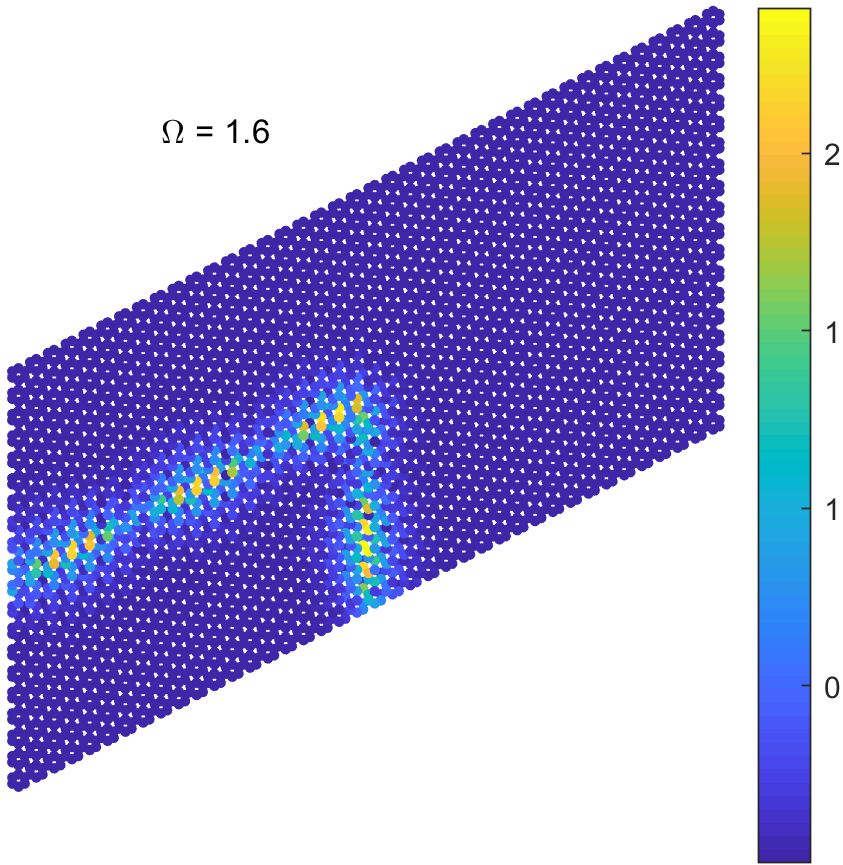
\includegraphics[width=1\linewidth]{imgs/sharpbendscat.png}
  \caption{The plot of $|y_i|$ for each mass in each cell.}
  \label{fig:sub2}
\end{subfigure}
\caption{Simulation of scattering on the hexagonal finite lattice with sharp
  bend.}
\label{fig:sharpbend}
\end{figure}

Amazingly, our system is able to stand up to both of these bends as we can see
in Figure~\ref{fig:gentlebend} and Figure~\ref{fig:sharpbend}.

%TODO: Continue with combination of straight bends; cross/interlace etc

\subsection{Curved bends}
So it can travel around gentle and sharp straight bends; it is only natural to
then wonder if it can propagate as well along a curved bend.

\begin{figure}
\centering
\begin{subfigure}[b]{.5\textwidth}
  \centering
  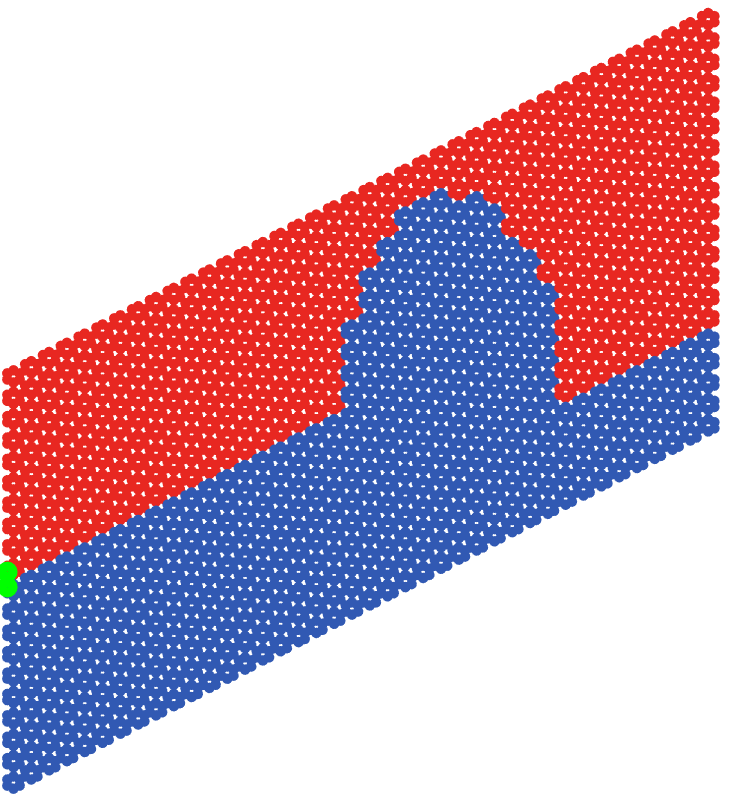
\includegraphics[width=0.8\linewidth]{imgs/curvedbendarr.png}
  \caption{Arrangement of cells to form a curved bend.}
  \label{fig:sub1}
\end{subfigure}%
\begin{subfigure}[b]{.5\textwidth}
  \centering
  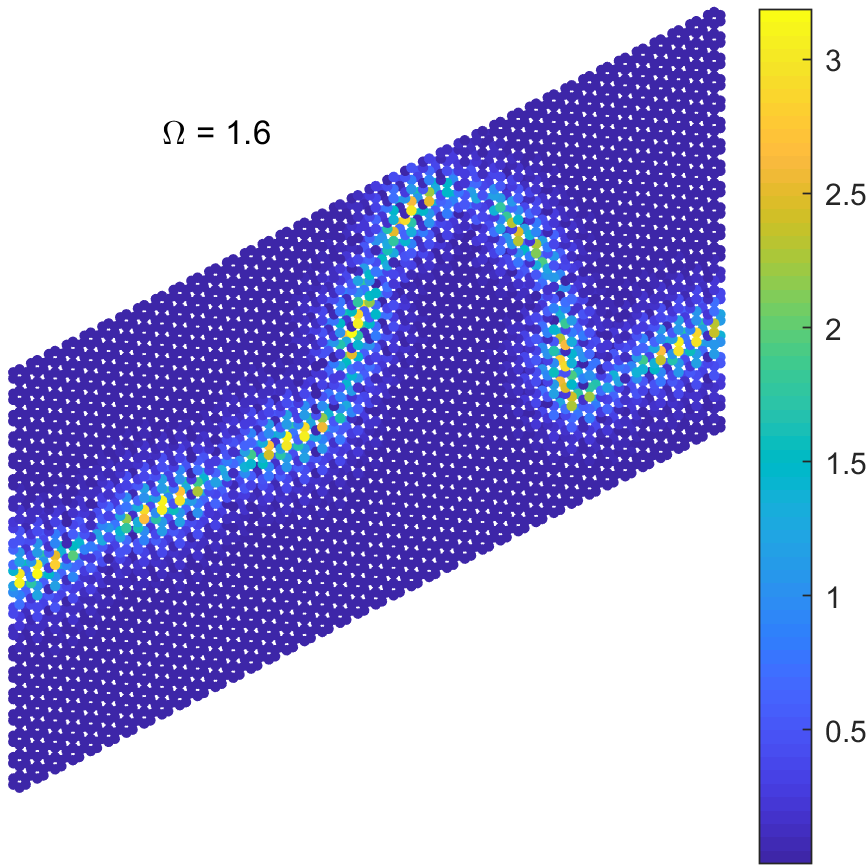
\includegraphics[width=1\linewidth]{imgs/curvedbendscat.png}
  \caption{The plot of $|y_i|$ for each mass in each cell.}
  \label{fig:sub2}
\end{subfigure}
\caption{Simulation of scattering on the hexagonal finite lattice with curved
  bend.}
\label{fig:curvedbend}
\end{figure}

\subsection{Grading}

\chapter{Evaluation}
% TODO: Compare results to those of more complex models; look at other papers
% and use their parameters
As mentioned in Chapter \ref{applications}, most of the practical applications
of metamaterials and photonic crystals come from their ability to control the
propagation of acoustic or electromagnetic waves. As such, it is important to
evaluate our model in terms of whether the results can translate to other
complex models.

To evaluate the performance and accuracy of our mass-spring model, we will
therefore compare our results to those produced in other papers, some with the
mass-spring model and some with more complex continuous models.

\section{Further work}
% TODO: Can split into what we can do in terms of different perturbations/
% grading etc; but also look at computing side, e.g. split into classes so
% easier to run simulations and get dispersion curves etc
% - compare the two different kind of perturbations. Is there a difference?
% Alternating mass one seems to be better. Amplitude is higher
There are many things that we can improve on and continue investigating for the
future. 

In terms of investigating deeper the challenges that might be faced when going
from simulations to a real world product, the following could be useful:
\begin{itemize}
\item Evaluating the robustness of our system to imperfections in the lattice.
This is crucial as real production systems have certain tolerances and are not
perfect. As such, it is important to be able to test how little changes in the
lattice can affect the edge states that we get, in terms of the strength of the
energy which is transmitted as well as the amount of energy which is dissipated
throughout the lattice.

\item Testing how small each layer of material can be to get a \textit{good
enough} edge state. So far in our discussions of the strips of cells, we have
been using strips with a large number of cells (e.g. $2N=40$) because we know
that the edge states decay exponentially outwards from the boundary, but this
may not be possible or cost effective when developing real products. Therefore,
it is important to study how the number of cells translates to the amount of
energy lost and how this might lead to unwanted energy elsewhere in the system
or interference with our edge state along the boundary. An example can be seen
in Figure~\ref{fig:smallvsbig}.
\end{itemize}

\begin{figure}
\centering
\begin{subfigure}[b]{.5\textwidth}
  \centering
  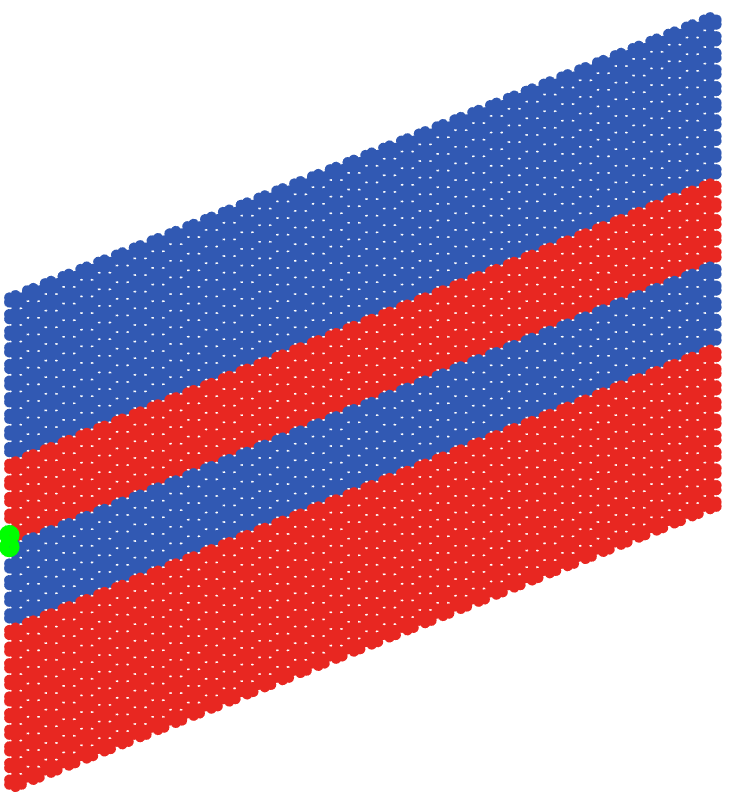
\includegraphics[width=0.7\linewidth]{imgs/svbthickarr.png}
  \caption{Arrangement of cells with $2N=10$.}
  \label{fig:sub1}
\end{subfigure}%
\begin{subfigure}[b]{.5\textwidth}
  \centering
  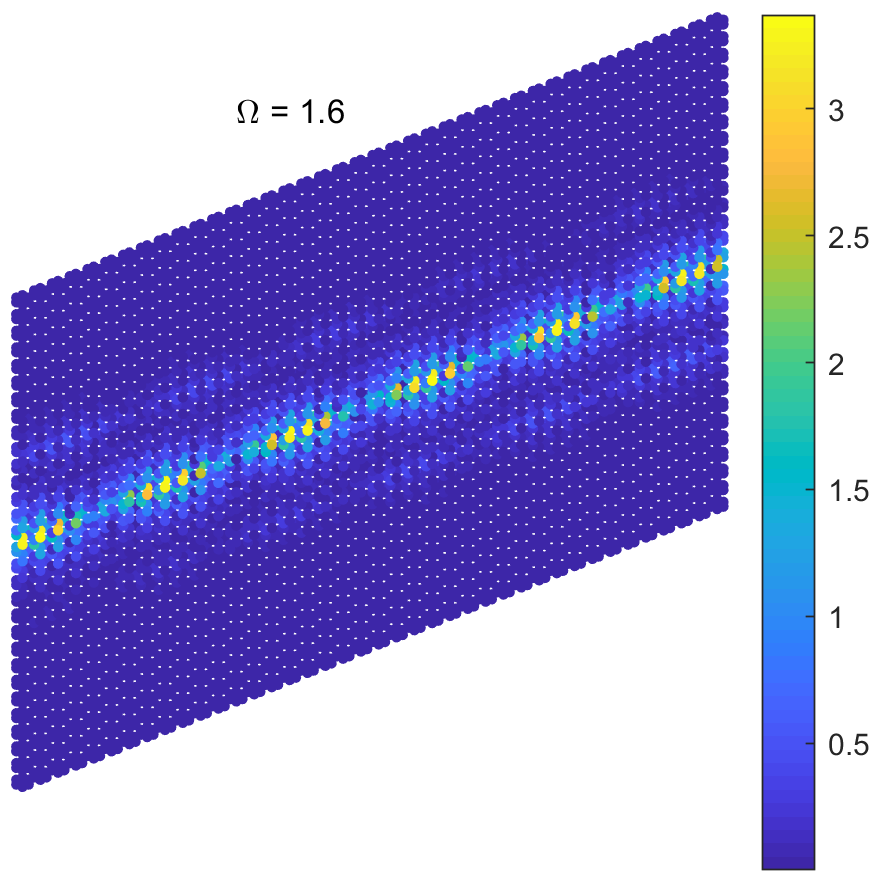
\includegraphics[width=0.9\linewidth]{imgs/svbthickscat.png}
  \caption{The plot of $|y_i|$ for each mass in each cell.}
  \label{fig:sub2}
\end{subfigure}

\medskip
\begin{subfigure}[b]{.5\textwidth}
  \centering
  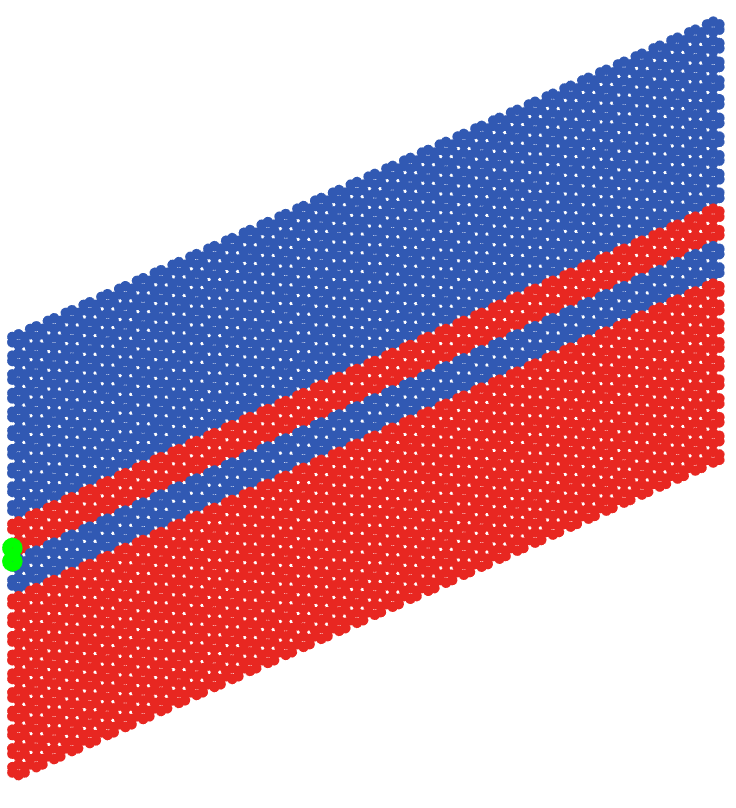
\includegraphics[width=0.7\linewidth]{imgs/svbthinarr.png}
  \caption{Arrangement of cells with $2N=4$.}
  \label{fig:sub1}
\end{subfigure}%
\begin{subfigure}[b]{.5\textwidth}
  \centering
  \includegraphics[width=0.9\linewidth]{imgs/svbthinscat.png}
  \caption{The plot of $|y_i|$ for each mass in each cell.}
  \label{fig:sub2}
\end{subfigure}

\medskip
\begin{subfigure}[b]{.5\textwidth}
  \centering
  \includegraphics[width=0.7\linewidth]{imgs/svbthinnerarr.png}
  \caption{Arrangement of cells with $2N=2$.}
  \label{fig:sub1}
\end{subfigure}%
\begin{subfigure}[b]{.5\textwidth}
  \centering
  \includegraphics[width=0.9\linewidth]{imgs/svbthinnerscat.png}
  \caption{The plot of $|y_i|$ for each mass in each cell.}
  \label{fig:sub2}
\end{subfigure}
\caption{Scattering simulation to show the differences in amplitude and
  dissipation of energy for hexagonal boundaries of different thicknesses using
  the cells as defined in Figure~\ref{fig:hexstripMrotated}.}
\label{fig:smallvsbig}
\end{figure}

In terms of improving the workflow for the generation of these results for
other geometries and topologies, we could implement the following:
\begin{itemize}
\item Move to an object-oriented programming model. We can implement the
concepts of shapes and topologies as interfaces which contain information about
the required geometries. Then we can create specific classes corresponding to
actual shapes to extend those interfaces. We can then have our core code which
generates the dispersion relations and scattering simulations work based on the
interface implemented, rather than being specific to one shape class. This
should be relatively straightforward to implement, as most of the code to solve
for dispersion curves and scattering simulations is the same for any shape. The
only big difference for different topologies is the formation of the
eigen-problem matrix, which is a really mechanical but time-consuming
procedure, and so this will make testing out new shapes or different connection
of masses much easier.

\item To take the above idea and make it even more user-friendly, we could
create a graphical user interface where a user can choose things like the shape
of the cell, the position of masses within the cell and how the masses are
connected. This would allow faster and simpler prototyping of new designs.
\end{itemize}

\chapter{Conclusion}
\appendix
\chapter{First Appendix}

\bibliographystyle{unsrt}
\bibliography{bibs/bibliography}

\end{document}
